\documentclass{article}
%\usepackage{makeidx,showidx}
\usepackage[fleqn]{amsmath}
\usepackage{graphicx}
\usepackage[
    web={designv,
    latextoc,forcolorpaper,
    centertitlepage},
    eforms
]{aeb_pro}
\usepackage[bypasspkgpagestyle,nomarginwrite,usecustomdesign,
    useclassmaketitle,flextended
]{eqexam}


%\usepackage[designv,
%    latextoc,forcolorpaper,
%    centertitlepage]{web}
%\usepackage{eforms}

%\usepackage[nopoints,fortextbook,nomarginwrite,usecustomdesign]{eqexam}
%\usepackage{longtable,colortbl}
%\useFullWidthForPaper

\usepackage{eqexaman}

\usepackage{srcltx}

\hfuzz=1pt


\def\AEBBook{\textsl{{Acro\!\TeX} eDucation System Tools: {\LaTeX} for interactive PDF documents}}
\def\AEBP{\textsf{AeB Pro}}

\DeclareFontFamily{U}{wi}{}
\DeclareFontShape{U}{wi}{m}{n}{<-> wingding}{}
\DeclareFontFamily{U}{webd}{}
\DeclareFontShape{U}{webd}{m}{n}{<-> webdings}{}

\font\zqacr=zqacr at 8pt

\newcommand\Com[2][]{\texttt{#2}}
\newcommand\sCom[2][]{}
\newif\ifusebw \usebwfalse

\setlength{\mathindent}{\leftmargini}

\edef\amtIndent{\the\parindent}

%\def\meta#1{\textit{$\langle$#1$\rangle$}}

\makeatletter

\let\ipkg\@gobble
%\def\numberline#1{{\setlength{\fboxsep}{0pt}\fbox{\hb@xt@\@tempdima{#1\hfil}}}}

%\renewcommand*\l@section{\addvspace{2pt}\@dottedtocline{1}{1.5em}{2.5em}}
\renewcommand*\l@subsection{\addvspace{1pt}\@dottedtocline{2}{1.5em}{3em}}
\renewcommand*\l@subsubsection{\addvspace{1pt}\@dottedtocline{3}{4.5em}{1.2em}}

%\renewcommand*\l@subsubsection{\addvspace{1pt}\@dottedtocline{3}{7.4em}{1.2em}}

%\renewcommand*\l@section{\@dottedtocline{1}{1.5em}{2.3em}}
%\renewcommand*\l@subsection{\@dottedtocline{2}{4.8em}{3.4em}}
%\renewcommand*\l@subsubsection{\@dottedtocline{3}{8.2em}{1.2em}}
%\renewcommand*\l@subsubsection{\@dottedtocline{3}{7em}{1.2em}}

\renewcommand{\paragraph}
    {\@startsection{paragraph}{4}{0pt}{6pt}{-3pt}
    {\normalfont\normalsize\bfseries}}
\renewcommand{\subparagraph}
    {\@startsection{subparagraph}{5}{\parindent}{6pt}{-3pt}%
    {\normalfont\normalsize\bfseries}}

\newcommand{\exAeBBlogPDF}[2][\urlAcroTeXBlog/]{\par\ifdim\lastskip>0pt\relax\vskip-\lastskip\fi
\vskip\medskipamount\noindent\makebox[0pt][r]{%
    \makebox[0pt][l]{\textcolor{blue}{\Pisymbol{webd}{254}}}%
    \raisebox{-2pt}{\color{red}\href{#1?#2}{{\zqacr b\hspace{9.5pt}}}}\enspace}\ignorespaces}

\newcommand{\exAeBBlogArticle}[2][\urlAcroTeXBlog/]{\par\ifdim\lastskip>0pt\relax\vskip-\lastskip\fi
\vskip\medskipamount\noindent\makebox[0pt][r]{\makebox[0pt][l]{\hspace{-1pt}\textcolor{blue}{\Pisymbol{webd}{254}}}%
\raisebox{.5pt}{\color{red}\href{#1?#2}{\ding{045}}\hspace{7.5pt}\enspace}}\ignorespaces}
\definePath{\urlAcroTeXBlog}{http://www.acrotex.net/blog}

\renewcommand*\descriptionlabel[1]{\hspace\labelsep
    \normalfont #1}
\newcommand{\aebDescriptionlabel}[1]{%
    \setlength\dimen@{\amtIndent+\labelsep}%
    {\hspace*{\dimen@}#1}}
\makeatother
\newenvironment{aebDescript}
    {\begin{list}{}{\setlength{\labelwidth}{0pt}%
        \setlength{\leftmargin}{\leftmargin}%
        \setlength{\leftmargin}{\leftmargin+\amtIndent}%
        \setlength\itemindent{-\leftmargin}%
        \let\makelabel\aebDescriptionlabel
    }}{\end{list}}

\def\hardspace{{\fontfamily{cmtt}\selectfont\symbol{32}}}
\def\AcroBlog{{Acro\!\TeX} Blog}
\newlength{\aebdimen}
\def\anglemeta#1{$\langle\textit{\texttt{#1}}\rangle$}
\let\ameta\anglemeta
\def\meta#1{\textit{\texttt{#1}}}
\let\pkg\textsf
\let\env\texttt
\let\opt\texttt
\let\app\textsf
\def\lp{(}\def\rp{)}
\def\AEB{\textsf{AeB}}
\def\AcroTeX{Acro\!\TeX}
\def\HTML{HTML}\def\FDF{FDF}
\def\PDF{PDF}\def\URL{URL}
%\let\amtIndent\leftmargini
\def\bNH{\begin{NoHyper}}\def\eNH{\end{NoHyper}}
\def\nhnameref#1{\bNH\nameref{#1}\eNH}
\def\nhNameref#1{\bNH\Nameref{#1}\eNH}
\def\nhurl#1{\bNH\url{#1}\eNH}
\def\grayV#1{\textcolor{gray}{#1}}
\def\darg#1{\{#1\}}
\def\parboxValign{t}
\renewcommand*{\backrefalt}[4]{%
    \ifcase #1\or
       See page~#2.\else See pages~#2.\fi
}
\newenvironment{aebQuote}
   {\list{}{\leftmargin\amtIndent}%
    \item\relax}{\endlist}
\newcommand{\FmtMP}[2][0pt]{\mbox{}\marginpar{%
    \raisebox{.5\baselineskip+#1}{%
    \expandafter\parbox\expandafter[\parboxValign]%
        {\marginparwidth}{\aebbkFmtMp#2}}}}
\def\aebbkFmtMp{\kern0pt\itshape\small
    \ifusebw\color{gray}\else\color{blue}\fi
    \raggedleft\hspace{0pt}}
\def\dps{$\mbox{$\mathfrak D$\kern-.3em\mbox{$\mathfrak P$}%
   \kern-.6em \hbox{$\mathcal S$}}$}
\def\FitItIn{\eq@fititin}
\def\endredpoint{\FitItIn{{\large\ifusebw\color{black}\else\color{red}\fi$\blacktriangleleft$}}}

\reversemarginpar

%\makeindex

\title[dps]{The \texorpdfstring{\textsf{eqexam} Package\\}{eqexam Package, }
part of the\texorpdfstring{\\}{ }\texorpdfstring{\AcroTeX}{AcroTeX} eDucation Bundle}
\author{D. P. Story}
\subject{%
    A LaTeX package for creating Test, quizzes, both for paper and for
    online use; supports writing problems sets for textbook authors.%
}
\keywords{LaTeX, hyperref, PDF, exercises, quizzes}
\university{{\AcroT} Software Development Team}
\email{dpstory@acrotex.net}
\version{5.1.13, 2021/01/20}
\copyrightyears{2005-\the\year}

\renewcommand{\exsectitletext}{Solutions to exams in this manual}


\chngDocObjectTo{\newDO}{doc}
\begin{docassembly}
var titleOfManual="The eqexam Manual";
var manualfilename="Manual_BG_Print_eqexam.pdf";
var manualtemplate="Manual_BG_Brown.pdf"; // Blue, Green, Brown
var _pathToBlank="C:/Users/Public/Documents/ManualBGs/"+manualtemplate;
var doc;
var buildIt=false;
if ( buildIt ) {
    console.println("Creating new " + manualfilename + " file.");
    doc = \appopenDoc({cPath: _pathToBlank, bHidden: true});
    var _path=this.path;
    var pos=_path.lastIndexOf("/");
    _path=_path.substring(0,pos)+"/"+manualfilename;
    \docSaveAs\newDO ({ cPath: _path });
    doc.closeDoc();
    doc = \appopenDoc({cPath: manualfilename, oDoc:this, bHidden: true});
    f=doc.getField("ManualTitle");
    f.value=titleOfManual;
    doc.flattenPages();
    \docSaveAs\newDO({ cPath: manualfilename });
    doc.closeDoc();
} else {
    console.println("Using the current "+manualfilename+" file.");
}
var _path=this.path;
var pos=_path.lastIndexOf("/");
_path=_path.substring(0,pos)+"/"+manualfilename;
\addWatermarkFromFile({
    bOnTop:false,
    bOnPrint:false,
    cDIPath:_path
});
\executeSave();
\end{docassembly}

\begin{document}

\maketitle

\tableofcontents

\section{Forward}

For the past several years (this year is \the\year), I've been writing a book
titled,
\begin{quote}
\AEBBook.
\end{quote}
The book~\cite{book:AEBB} covers {\AEB}, which includes the \pkg{eforms}
package, and {\AEBP} in \emph{great detail} and includes many examples to
illustrate concepts and techniques. Numerous new examples are available on
the CD-ROM that accompanies the book.

During the time of the writing, each of the packages covered was examined,
bugs were fixed, and many new and major features were created. Any new
features developed in the course of writing the book are documented in the
book; however, they are \emph{not included in this documentation}. You can
either buy the yet-to-be-submitted book sometime in the future, or discover
the features by studying the DTX documentation of the program files. Sorry,
it took me three years to write the book, I don't want to spend another year
on this documentation. \verb!:-{)!

\begin{flushright}
Dr. D. P. Story\\[3pt]
\today
\end{flushright}

\section{Introduction}

In my classroom work at The University of Akron, I've been using a
personal {\LaTeX} package, which is called \textsf{eqexam}, for creating
my in-class tests, quizzes, homework assignments, and review documents
(pre-tests/sample tests). In recent weeks---at the end of the Fall
Semester, 2004, and prior to the Spring Semester, 2005, I have filled the
mundane and boring days with work on \textsf{eqexam}, fixing and enhancing
it quite a bit.

The \textsf{eqexam} package is a stand-alone for {\LaTeX}, but is also
tightly integrated with the {\cAcroEB}. \textsf{eqexam} will be
distributed by itself, as well as a part of the {\cAcroB}. The integration
with the {\AcroB} gives it many of the online features that users of the
Bundle are familiar with.

\newtopic (Version 3.0 or later) The method of formatting an \textsf{eqexam}
document has changed, each \texttt{problem}/\texttt{problem*} environment
is now in a list environment, the \texttt{eqequestions} environment. This
environment is not normally used by the document author, but its
parameters may be redefined. The purpose of this reformatting, is to open
up \textsf{eqexam} for use by other packages. Textbook authors can now, I
hope, easily integrate \textsf{eqexam} into the custom book format
being used.

\newtopic Let's have an overview of the package, with suggestions for
possible uses.
\begin{enumerate}
    \item The first, and most obvious application of this package
    is to create a \textcolor{blue}{pExam} or a
    \textcolor{blue}{pQuiz}. (Here, the `\textcolor{blue}{p}'
    prefix refers to \underline paper or \underline pulp; thus, we
    can use \textsf{eqexam} to write paper Exams and/or pulp
    Quizzes).  You can write the questions and the solutions, and
    publish (i.e., print the document on a printer) the exam/quiz
    with no solutions---ready to be taken in class---, or {\LaTeX}
    the source document with solutions listed after each question
    to create an answer key, for your personal use, or for the use
    by the class.

    \item So much for pulp. Now on to `\textcolor{blue}{e}' (for
    electronic publication). In some of my classes, I put sample
    questions (review tests) on the web as {\PDF} documents. In
    this case, you can create a {\PDF} document without the
    solutions, and give the class time to solve the problems; then
    publish the document (in {\PDF} on the web) with solutions.
    The solutions can appear immediately after the questions, or
    can be accumulated at the end of the document.

    \item[] In the case where the solutions are at the end of the
    document, you can add links from the question to the solution.

    \item[] Documents can be published with color (to enhance the
    on screen appearance) or can be published in black and white,
    meant to be printed. Or, you can do both: a screen
    version and a paper version.

    \item By invoking the \texttt{online} option, the white space
    left for hand-written answers to the questions become Acroform
    multi-line text fields, multiple choice questions become radio
    buttons, and fill-in questions also become text fields. The
    student can bring up the exam, and take it at a computer (in a
    CBT\footnote{Computer Based Testing.} lab). After the student
    is finished, he/she can print out the exam, and submit it to
    the instructor for traditional grading.

    \item Now, here is an exciting feature of the \textsf{eqexam}
    package, that of email submittal! This feature is not too
    useful for technical fields (i.e., mathematics related fields)
    that require students to enter special symbols, but for some
    academic disciplines (English, History, Sociology, Politics
    and Government, etc.) this feature could be quite
    exciting.\footnote{Of course, I am addressing now the some six
    people worldwide in these fields that use {\LaTeX} and \PDF!
    For you six, this feature is for you!}

    \item[] When you take the \texttt{email} option of
    \textsf{eqexam}, as with the \texttt{online} option, the white
    space left for hand-written answers to the questions become
    Acroform multi-line text fields, multiple choice questions
    become radio buttons, and fill-in questions also become text
    fields. Additionally, a button is automatically provided to
    submit by email the results of the test to the instructor. The
    results arrive at the instructor's mailer as an {\FDF}
    attachment.  The instructor can open the {\FDF} and view in the
    originating {\PDF} the responses given by the student.

    \item[] The instructor can print out the document and grade in
    a traditional way, or if the instructor has
    \textbf{Acrobat~Pro} or \textbf{Standard}, the instructor can
    use mark-up annotations within the PDF, save a copy of the
    students test to a class folder, and email a copy of the
    students exam, marked up with grade.\footnote{Seems doubtful
    that anyone at this time has the expertise to do this! But
    it's available if anyone ever wants it.}

    \item[] If the exam is given for credit, it can be taken in a
    secure lab.

    \item Perhaps a more reasonable application of this email
    submission feature of \textsf{eqexam} is the building and
    publication of surveys and questionnaires! Perhaps
    teacher evaluations! The environments of \textsf{eqexam} can
    be easily used to write surveys and questionnaires to
    solicit the opinion of a target population. Responses are
    emailed to the designated person, who can summarize them.

    \item[] By the way, speaking of summarizing results, a new
    feature of \textbf{Acrobat Pro~7.0}, allows you to take a
    folder of {\FDF} files, such as the ones created by email
    submission, and extract all form fields and place results to a
    comma-delimited file (\texttt{.csv}). This comma-delimited
    file can be opened by a spreadsheet program and manipulated.
    Cool.

    \item (08/05/11) Version 3.0 of \textsf{eqexam} has a major option,
        \texttt{fortextbook},\footnote{The \texttt{fortextbook} option is briefly
        described on page~\pageref*{fortextbook}.} designed to support (U.S.)
        textbook authors. Documentation for this option is found in the
        \texttt{doc/fortextbook} folder. See also the series of blogs at the
        \ulSetLink{http://www.acrotex.net/blog/?tag=fortextbook}{{Acro\TeX} Blog}.

\end{enumerate}

%\subsection{What's New}
%
%\begin{enumerate}
%
%    \item (Version 1.7) Added the ability to randomize items in a
%    multiple choice/selection list. See \Nameref{s:random} and the
%    \texttt{allowrandomize} option, as listed in \Nameref{eqoptions}.
%
%    \item (Version 1.6) In this version, I've added the command
%    \cs{thisterm} (see \Nameref{preamble}) and expanded the control of
%    multiple versions. Now you can have up to $26$ versions of the same
%    test! For details of this new multiple version scheme, see the
%    discussion in \Nameref{mutiVerNew}.
%
%    \item[] Also added are \cs{forproblem} and \cs{foritem}. See \mlNameref{solnSets}.
%
%    \item (Version 1.4) Added a \texttt{manswers} environment for
%    multiple choice questions where multiple selections are permitted.
%    \textsf{Exerquiz} version 6.04 or greater is required with the
%    \texttt{online} and \texttt{email} options. See the section
%    \Nameref{multiSelect} for details.
%
%    \item (Version 1.3) Added in the \cs{bChoices} and
%    \cs{eChoices} pair for specifying multiple choice
%    alternatives. See the brief discussion in
%    the section \Nameref{multichoice}.
%\end{enumerate}

\section{Required and Optional Packages}

The following packages that are not part of the normal {\LaTeX}
distribution are \emph{required}:
\begin{enumerate}
\item \texttt{calc}: Used for calculation of the position of the
    marginal points.

\item \texttt{pifont}: Used when the \texttt{proofread} option is
    used to indicate the correct answers to multiple choice questions.

\item \texttt{aeb-comment}: Used to have optional content, useful for
    developing exams for multiple sections of the same class.\footnote{\pkg{aeb-comment}
    is an older version of the \pkg{comment} package by Victor Eijkhout; it is distributed
    with the \pkg{acrotex} package.}

\item \texttt{multicol}: Used to create questions in multi-column mode.

\item \texttt{verbatim}: Used to write solutions to the hard drive.
\end{enumerate}

\noindent Additionally, the following packages may be used
depending on the options chosen:
\begin{enumerate}
\item \texttt{web}: Used when the \texttt{pdf}, \texttt{links},
    \texttt{online} or the \texttt{email} option is taken.

\item \texttt{exerquiz}: Used when the
    \texttt{links}, \texttt{online} or the \texttt{email} option is
    taken.
\end{enumerate}
Of course, \texttt{web} and \texttt{exerquiz}, in turn, input a
whole plethora of packages. Consult the documentation for the
\cAcroEB.

\section{Installing \textsf{eqexam}}

Create a folder in your \texttt{latex} search path named
\textsf{eqexam} and place the package files \texttt{eqexam.dtx},
\texttt{eqexam.ins}, \texttt{eqexam.def} and any \texttt{.cfg}
files. (If you have an \texttt{acrotex} folder, you can place the
files there as well.)

Next, \texttt{latex} \texttt{eqexam.ins} to create
\texttt{eqexam.sty} and \texttt{eqalone.def}. The other files
(\texttt{*.tex} and \texttt{*.pdf}) can be placed anywhere.

The \textsf{eqexam} is a stand alone package that is tightly
integrated with the \cAcroB. The file \texttt{eqexam.def} comes
from the {\cAcroB} to provide the necessary support for many of
the commands and environments defined in \textsf{eqexam}. The file
\texttt{eqalone.def} are miscellaneous definitions that are needed
for the stand-alone version. When you choose one of the options
\texttt{links}, \texttt{online} or \texttt{email}, then
\textsf{Exerquiz} is included in the package files. When you use
one of these options you will need the most recent version of the
\cAcroEB, the one published concurrently with this package.

\section{Demonstration files}

\exAeBBlogPDF{cat=107} The original
\href{\urlAcroTeXBlog/?cat=107}{\pkg{eqexam} demonstration files} are posted
on the \href{\urlAcroTeXBlog/}{{Acro\TeX} Blog}. Throughout the manual, individual
files are references and a link is provided to that resource. The source file is attached
to all PDFs on the {Acro\TeX} Blog website.

\exAeBBlogPDF{tag=eqexam-package}
Additional demonstration files developed after the original set are also available
from the {Acro\TeX} Blog. See the articles tagged as
\textit{\href{\urlAcroTeXBlog/?tag=eqexam-package}{eqexam-package}}.

%http://www.acrotex.net/blog/?tag=eqexam-package


\section{Page Layout Considerations}

With Version~3.0, you can design your own page layout scheme, perhaps to
conform to a book style. The following are some basics on formatting for
\textsf{eqexam}.

The following two commands appear in \textsf{eqexam}, the first sets some basic
page parameters.
\begin{Verbatim}[xleftmargin=\amtIndent,fontsize=\fontsize{9}{11}\selectfont]
\newcommand{\eqeSetExamPageParams}{%
    \setlength{\headheight}{12pt}
    \setlength{\topmargin}{-.5in}
    \setlength{\headsep}{20pt}
    \setlength{\oddsidemargin}{0pt}
    \setlength{\evensidemargin}{0pt}
    \setlength{\marginparsep}{11pt}
    \setlength{\marginparwidth}{35pt}
    \setlength{\footskip}{11pt}
}
\end{Verbatim}
The second command calculates values for \cs{textwidth} and \cs{textheight}
based on the the settings of the first command.
\begin{Verbatim}[xleftmargin=\amtIndent,fontsize=\fontsize{9}{11}\selectfont]
\newcommand{\eqExamPageLayout}{%
    \setlength\textwidth\paperwidth
    \addtolength{\textwidth}{-2in}
    \addtolength{\textwidth}{-\oddsidemargin}
    \setlength\textheight{\paperheight}
    \addtolength\textheight{-2in}
    \addtolength\textheight{-\headheight}
    \addtolength\textheight{-\headsep}
    \addtolength\textheight{-\topmargin}
    \addtolength\textheight{-\footskip}
}
\end{Verbatim}
When the package option \texttt{usecustomdesign} \textit{is not taken,}
then the two commands \cs{eqeSetExamPageParams} and \cs{eqExamPageLayout}
are executed immediately after the above definitions. These are the
original parameters used by \textsf{eqexam}, designed to yield a maximum
text body in which to typeset an exam. The margins are set at 1 inch, the
\cs{topmargin} is raised up, all to maximize space.

Now, if the package option \texttt{usecustomdesign} is specified, the
commands \cs{eqeSet\-Exam\-Page\-Params} and \cs{eqExamPageLayout} are \emph{not
executed}, the package designer can either do a \cs{renewcommand} for
these two commands in the preamble with custom values inserted (and
execute \cs{eqeSetExamPageParams} and \cs{eqExamPageLayout}), or the
designer may use another package to set the page layout parameters (or
take the default of the class being used). In the latter case,
neither \cs{eqeSetExamPageParams} nor \cs{eqExamPageLayout} should be executed.

\newtopic The following commands directly effect how the problems are
displayed within an \textsf{eqexam} environment.

\begin{Verbatim}[xleftmargin=\amtIndent,fontsize=\fontsize{9}{11}\selectfont]
\eqexammargin{\normalsize\normalfont\bfseries00.\ }
\end{Verbatim}
The command \cs{eqexammargin} is a convenient way of specifying the
\cs{labelwidth} as set by the \texttt{eqequestions} environment (see
below). The command uses \cs{settowidth} to set the \cs{eqemargin} length.
The \cs{eqemargin} may also be set directly with \cs{setlength}.
\cs{eqexammargin} can be executed anytime between exam environments (or
even between problems, though this is not a intuitive option). Normally it
is executed once for the entire document; but may be executed multiple
times to change margins.

\begin{Verbatim}[xleftmargin=\amtIndent,fontsize=\fontsize{9}{11}\selectfont]
\newcommand{\widthtpboxes}{35pt}
\end{Verbatim}
This command sets the width of the boxes that appear in the right margin
when one of more of the options \texttt{pointsonright},
\texttt{pointsonboth}, \texttt{totalsonleft}, \texttt{totalsonright}, are
used. These boxes are used for exams, and not relevant for problem sets of
textbooks. Normally, this parameter is not redefined.

\begin{Verbatim}[xleftmargin=\amtIndent,fontsize=\fontsize{9}{11}\selectfont]
\newenvironment{eqequestions}{%
    \begin{list}{}{%
        \setlength{\labelwidth}{\eqemargin}%
        \setlength{\topsep}{3pt}\setlength{\parsep}{0pt}%
        \setlength{\itemindent}{0pt}\setlength{\itemsep}{3pt}%
        \setlength{\leftmargin}{\labelwidth}%
        \settowidth{\labelsep}{\ }%
    }\item\relax}{\end{list}}
\end{Verbatim}
This environment is opened at the beginning of a \texttt{problem}
(\texttt{problem*}), and closed at the end of these environments.

\section{Building an Exam}

In this section, we outline the steps to create an exam using the
\textsf{eqexam} package. Consult the sample exams for additional
examples.

\subsection{The Preamble}\label{preamble}

Of course, we begin with the standard article class, and the
\textsf{eqexam} package:
\begin{Verbatim}[xleftmargin=\amtIndent,commandchars=!()]
\documentclass{article}
\usepackage[!meta(options)]{eqexam}
\end{Verbatim}
\noindent The \meta{options} are discussed in
section~\ref{eqoptions}.  Next comes a exam identification
information:
\begin{Verbatim}[xleftmargin=\amtIndent,fontsize=\fontsize{9}{11}\selectfont]
\title[T1]{Test 1}
\subject[C1]{Calculus I}
\author{D. P. Story}
\keywords{Calculus I, Section 004}
\university{%
      THE UNIVERSITY OF AKRON\\
    Mathematics and Computer Science
}
\date{\thisterm, \the\year}
\duedate{October 17, 2005}
\end{Verbatim}
\noindent The \cs{title}, \cs{subject}, \cs{author} and \cs{date}
are the same as is used in the \textsf{web} package. These are
used by the standard {\LaTeX} macro to create the heading line of
the first page of the exam, and are used in the running headers.

The \cs{title}, \cs{subject} have optional first arguments, where
you can list a shorted version of the title or the subject. The
shortened versions, if present, are used in the running headers.

The \cs{keywords} is used when you publish your exam in {\PDF} and
you use the \texttt{pdf} option (or \texttt{online}, \texttt{links},
\texttt{email}). The value of the argument of \cs{keywords} appears
in the keywords field of the document info dialog.

When you take the \texttt{coverpage} option, the value of
\cs{university} is used, along with some of the others on the
cover page.

I've also defined a keyword of \cs{duedate}, this might be useful
when using \textsf{eqexam} to create homework assignments with a
due date, or just to record the date of the exam. The argument of \cs{duedate} fills the text macro
\cs{theduedate}. So that if you say \verb|\duedate{05/31/06}|, the macro
\cs{theduedate} will expand to `05/31/06'.

\newtopic Beginning with version~1.6, \cs{thisterm} is defined.
The academic year of many American universities are divided into semesters
(or terms); Fall, Spring, and Summer.  The command \cs{thisterm} takes the current
date and determines if it is the Fall, Spring or Summer Semester. For example,
if the date of the compile is October 17, 2005, then \verb!\thisterm, \the\year!
expands to `Fall, 2005'.  This command is useful with the \cs{date} command.

The command \cs{thisterm} can be redefined to conform to the terms
of the document author's university. See the definition in
\texttt{eqexam.dtx}, copy and modify it.

\subsection{The \texttt{exam} Environment}\label{exam}

An exam is contained within the \texttt{exam} environment.

One of the things that I do in my courses, especially for the
final exam, is to have a two-part exam. Typically, the first part
is worth $100$ points and covers the new material not already
tested; the second part is usually a $50$ point review.  I grade
these two parts separately and record them separately. Therefore,
an \textsf{eqexam} test may contain one or more \texttt{exam}
environments.\footnote{Remember, this was originally a personal
package, meant to suit my own needs.}

\newtopic After the preamble, we then say
\begin{Verbatim}[xleftmargin=\amtIndent,fontsize=\fontsize{9}{11}\selectfont]
\begin{document}

\maketitle

\begin{exam}[Part I.]{Part1}

\begin{instructions}[Part I.]
Solve each of the problems without error. If you make an error,
points will be subtracted from your total score.
\end{instructions}
...
...
...
\end{exam}

\begin{exam}[Part II.]{Part2}

\begin{instructions}[Part II.]
The following is a short review of previously mastered material.
\end{instructions}
...
...
...
\end{exam}
\end{document}
\end{Verbatim}
After the \verb+\begin{document}+ and standard \cs{maketitle}, we begin an
exam by opening an \texttt{exam} environment.

\settowidth{\aebdimen}{\ttfamily\string\begin\darg{exam}[\meta{friendly\_name}]\darg{\meta{exam\_name}}}
\begin{dCmd}[commandchars=!()]{\aebdimen+2\fboxsep+2\fboxrule}
\begin{exam}[!meta(friendly_name)]{!meta(exam_name)}
...
\end{exam}
\end{dCmd}
\noindent This environment has two arguments: the first optional, the second
required. The first argument is a user friendly name (used when the solutions
are listed at the end of the document when there are multiple \texttt{exam}
environments); the second required argument is the name of the of the exam,
\texttt{Part1} or \texttt{Part2}, for example. This argument is used to build
the names of the PDF Acroform field names. This argument should consist of
letters and numbers only. You can use the command \cs{autoExamName} for the
\meta{exam\_name}; this command will name each \texttt{exam} environment
\texttt{exam1}, \texttt{exam2}, \texttt{exam3}, etc.

Following the opening of the exam, typically, the instructor would have
some instructions, this is the purpose of the \texttt{instructions}
environment. It has one optional argument, heading text for the
instructions; if this optional parameter is not provided, then the default
word is used, the default word is determined by \cs{defaultInstructions},
its default definition is
\begin{Verbatim}[xleftmargin=\amtIndent]
\defaultInstructions{Instructions.}
\end{Verbatim}
Following this label, the total number of points for this part is
inserted, unless the \texttt{nosummarytotals} option is taken.

\redpoint The optional argument of the \texttt{instructions}
environment has a color associated with it, and is visible when you
compile the document with the \texttt{forcolorpaper} option. This
color can be set by the command \cs{instructionsColor}; this command
takes a single argument, a named color:
\begin{Verbatim}[xleftmargin=\amtIndent]
\instructionsColor{blue}
\end{Verbatim}
\noindent The above is the default definition.


\newtopic At this point, you would insert your questions. Following the
listing of all the questions (and optionally, their solutions), you
finish up by closing out the \texttt{exam} environment.

Repeat, if additional parts to the exam are desired. Finally,
finish off the document with \verb+\end{document}+.

\redpoint You must \texttt{latex} your document \emph{three times} to be
sure all points have been properly calculated.

\subsection{The \texttt{problem} and \texttt{problem*} Environments}

All questions are posed using the \texttt{problem} and
\texttt{problem*} environments. The former is for a single
question, the latter is for a question with multiple parts.

\subsubsection{\texttt{problem}}\label{problem}

The \texttt{problem} encloses a single question; the question
itself may contain special constructs such as one or more fill-in
the blanks.

The syntax for \texttt{problem} is
\begin{Verbatim}[xleftmargin=\amtIndent,fontsize=\fontsize{9}{11}\selectfont,
    commandchars=!()]
\begin{problem}[!meta(num)|*!meta(num)|empty][h|H]
!anglemeta(Statement of question, which may contain special constructs)
...
...
\begin{solution}[!meta(vspace),nLines=!meta(n)]
...
...
\end{solution}
\end{problem}
\end{Verbatim}
\noindent The environment takes two optional arguments. The first
argument \meta{num} is the number of points for this problem, for
example, if we want to have a $5$ point question, we would begin the
environment like so, \verb+\begin{problem}[5]+; on the other hand, if we
say \verb+\begin{problem}+, the problem has no points associated with it.
If you specify points weight for a problem, the points appear in the
margins (when one of the option \texttt{pointsonleft},
\texttt{pointsonright}, or \texttt{pointsonboth} is specified); if the
\texttt{*} form is specified (\meta{*num}), the point weight appears
``in-line,'' just after the problem number; thus, typesetting a problem
with the specification \verb!\begin{problem}[*5]! yields
\begin{quote}
\textbf{1.} (5 pts) \dots
\end{quote}
This is useful when the problems are put into a two-column format; the
problems in the right-hand column do not have the margin to hold the
points, in this case, we place the points ``in-line.''

\newtopic The \texttt{problem} is actually a redefined \texttt{exercise}
environment, as defined in \textsf{exerquiz}. The second parameter
is inherited from the \texttt{exercise} environment. The second
argument can optionally be an \texttt{h} or a \texttt{H}.

Use \texttt{h} if you do not want the solution to appear at the
end of document (when you do not use the \texttt{nosolutions} or
the \texttt{solutionsafter} options); the solution, however, will
appear if the \texttt{solutionafter} option is specified.

For the \texttt{H} argument, the solution will not appear at the
end of the document (just as in \texttt{h}), nor will it appear if you
specify the \texttt{solutionsafter} option.

To make things work correctly, if you do not want to have points
for a question and want to hide the solution, use `\texttt{[]}'
(empty brackets with no spaces) for the first argument.
\begin{Verbatim}[xleftmargin=\amtIndent,fontsize=\fontsize{9}{11}\selectfont]
\begin{problem}[][H]
($5$ Points Extra Credit) Solve this problem for extra credit.
\begin{solution}
This solution will not appear in all cases, unless the second
parameter is eliminated or is changed to h, in the latter case,
the solution appears just for \texttt{solutonsafter}.
\end{solution}
\end{problem}
\end{Verbatim}
\noindent Here, this problem has no points that will be added into
the total number of points for the test.

The \texttt{solution} environment encloses the solutions. This environment is
optional. The environment takes at most two optional parameters,
\meta{vspace} and \texttt{nLines=\meta{n}}. The \meta{vspace} parameter is a
length that determines the amount of vertical space to leave for the student
to work the problem. The
\texttt{nLines=\meta{n}}\FmtMP{\texttt{nLines=\meta{n}} explained}
specification signals \pkg{eqexam} to leave \meta{n} lines of vertical space;
each line is \cs{wlVspace} in height. (For more information on \cs{wlVspace},
read about the \texttt{linegap} key in Section~\ref{ss:VSFT}.) This vertical
space is \emph{created only} when the document author takes the
\texttt{nosolutions} or \texttt{vspacewithsolns} option. For example,
\begin{Verbatim}[xleftmargin=\amtIndent,fontsize=\fontsize{9}{11}\selectfont]
\begin{problem}[10]
Do this problem.
\begin{solution}[2in]
This is the solution.
\end{solution}
\end{problem}
\end{Verbatim}
This defines a $10$ point problem and leaves $2$ inches of vertical space
following the problem statement for the student to respond. The vertical
space is generated provided the \texttt{nosolutions} or \opt{vspacewithsolns}
option has been taken.

Be aware that the solution environment searches for its optional
parameter, and will expand macros looking for a left bracket (\texttt{[}).
In documents where the optional parameter is not used; this can lead to
problems in compiling. For example, if you say,
\verb!\begin{solution} \textbf{My solution:}...!, the command \cs{textbf}
will be expanded prematurely and result in `My solution' not appearing in
bold. Similarly, if you write \verb!\begin{solution} \begin{equation}...!
can lead to compilation stopping. Suggested workarounds:
\begin{itemize}
    \item Supply empty brackets: \verb!\begin{solution}[]!
    \item Use \cs{relax}: \verb!\begin{solution}\relax\textbf{...}!.
    The \cs{relax} should not be on the line by itself.
\begin{Verbatim}[xleftmargin=\amtIndent,fontsize=\fontsize{9}{11}\selectfont]
\begin{solution}\relax  % Not this
\textbf{...}
...
\end{Verbatim}
The above causes an unwanted newline. The next two examples show the
``correct'' method.
\begin{Verbatim}[xleftmargin=\amtIndent,fontsize=\fontsize{9}{11}\selectfont]
\begin{solution}\relax\textbf{...}  % correct
...
\end{Verbatim}
\noexpand The \cs{relax} appearing on the second line.
\begin{Verbatim}[xleftmargin=\amtIndent,fontsize=\fontsize{9}{11}\selectfont]
\begin{solution}
\relax\textbf{...}  % correct
...
\end{Verbatim}
\end{itemize}
If you have no need for the vertical space in your document and putting in
these workarounds is too much trouble, you can use a global solution. Use
\cs{noSolnOpt} to globally turn off the check for the option parameter by
the \texttt{solution} environment; \cs{ckSolnOpt} turns on parameter
checking (the default). To summarize:
\begin{Verbatim}[xleftmargin=\amtIndent,fontsize=\fontsize{9}{11}\selectfont]
\ckSolnOpt  % turn on checking for the optional argument (the default)
\noSolnOpt  % turn off checking for the optional argument
\end{Verbatim}
Place either of these two commands between problems to turn off (or back on) the
parameter checking.

\redpoint See \Nameref{eqoptions} for more details on
the two options \texttt{nosolutions} and \texttt{solutionsafter}.

\paragraph*{Optional arguments of \env{solution} environment.}
The \env{solution} environment takes at most two optional arguments \meta{vspace} and \texttt{nLines=\meta{n}}.
If both are specified, by default the \meta{vspace} parameter is used. The command
\cs{usenLineDimen} changes the preference to the line specification; \cs{useVspaceDimen} switches
the preference back to the \meta{vspace} dimension.

\subsubsection{\texttt{problem*}}\label{problemstar}

This environment is used when you want to ask a multi-part
question, a series of related questions that are to be treated as
a group.

The syntax is
\begin{Verbatim}[xleftmargin=\amtIndent,fontsize=\fontsize{9}{11}\selectfont,
    commandchars=!()]
\begin{problem*}[!meta(num)|!anglemeta(num)ea|\auto|empty][\Do!anglemeta(do_num)]
Do each of the following problems, and be quick about it.
\begin{parts}

\item[h|H] The first question.
\begin{solution}[!meta(vspace),nLines=!meta(n)]
This is the solution to the first problem.
\end{solution}

\item[h|H] The second question.
\begin{solution}[!meta(vspace),nLines=!meta(n)]
This is the solution to the second problem.
\end{solution}

\end{parts}
\end{problem*}
\end{Verbatim}
The \texttt{problem*} environment takes two optional parameters,
the first one takes one of four values:
\begin{aebDescript}
    \item[\meta{num}] When the value of the first parameter is
    a number, this represents the total number of points for this
    multi-part question. Here, the instructor does not specify the
    weight of each part.

    \item[\meta{*num}] The points appear ``in-line'' rather than
        in the margin.

    \item[\anglemeta{num}\texttt{ea}] When you specify a number followed by
    `\texttt{ea}' (which is short for \underbar{ea}ch). Thus,
    `\texttt{[5ea]}' signifies that each part of this problem has
    weight of $5$ points.

    \item[\texttt{*\anglemeta{num}ea}] The points appear ``in-line'' rather than
        in the margin.

    \item[\cs{auto}] If the value of the first parameter is
    \cs{auto}, then the total number of points is calculated
    automatically from the points defined by the \cs{PTs} macro.
    The \cs{PTs} would be placed following \cs{item} of each part
    that is to be given points. For example:

    \item[*\cs{auto}] The points appear ``in-line'' rather than
        in the margin.

\begin{Verbatim}[xleftmargin=\amtIndent,fontsize=\fontsize{9}{11}\selectfont]
\begin{problem*}[\auto]
Do each of the following problems, and be quick about it.
\begin{parts}

\item\PTs{3} The first question.
\begin{solution}[1.5in]
This is the solution to the first problem.
\end{solution}

\item\PTs{4} The second question.
\begin{solution}[3in]
This is the solution to the second problem.
\end{solution}

\end{parts}
\end{problem*}
\end{Verbatim}
This defines a $7$ point problem.

\item[\texttt{empty}] You need not specify any points at all. In
this case do not include this first parameter, in which case, the
second parameter is not used, so don't include it either.

\end{aebDescript}

\noindent Now for a description of the second parameter the
\texttt{[\cs{Do}\anglemeta{do\_num}]} parameter. In my senior- or graduate-level
classes, I sometimes ask a questions with multiple parts. As part
of the instructions for that problem I write, ``Do exactly three
of the following five problems.'' These questions are usually
proof-type problems, and they can choose their best three to
grade. In this context, all parts of the problem must be of the same
weight; the weight of each is \anglemeta{num} of the \texttt{[\anglemeta{num}ea]}.

This is what \texttt{[\cs{Do}\anglemeta{do\_num}]} does. When you specify
\texttt{\cs{Do}3}, then only the points of $3$ of the problems are
added into the exam total. This second parameter is only checked
if the first parameter is \texttt{[\anglemeta{num}ea]}. For example,
specifying
\begin{Verbatim}[xleftmargin=\amtIndent,fontsize=\fontsize{9}{11}\selectfont]
\begin{problem*}[5ea][\Do3]
\end{Verbatim}
creates a $15$ point question. This assumes there are $3$ or
more parts to this question.

By the way, there are two macros that are defined when the \cs{Do}
is used, they are \cs{DoNum} and \cs{OutOfNum}; these expand to
the (English) word for the number of problems to do, and the
(English) word for the total number of problems. For example, if
there were five parts to the problem below,\dots
\begin{Verbatim}[xleftmargin=\amtIndent,fontsize=\fontsize{9}{11}\selectfont]
\begin{problem*}[5ea][\Do3]
Solve exactly \textit{\DoNum} of the following {\OutOfNum}
problems. ....
\end{problem*}
\end{Verbatim}
\noindent The instructions would read, ``Solve exactly
\textit{three} of the following five problems.'' These macros can
be easily redefined to reflect other languages. The numbers
themselves are contained in the two macros \cs{nDoNum} and
\cs{nOutOfNum}.

\redpoint \texttt{parts} and \cs{item}: For a multi-part problem
(\texttt{problem*}), the actual problems are enclosed in a
\texttt{parts} environment, and each question is posed as an
\cs{item} of that \texttt{list} environment. The command \cs{item}
takes the \texttt{[h|H]} optional argument. As in the case of the
\texttt{problem} environment, \texttt{h} prevents the solution
from appearing at the end of the document (but it appears with
\texttt{solutionsafter}), and \texttt{H} removes the solution in
all cases.

\paragraph{\texorpdfstring{\cs{leadinitem}}{\CMD{leadinitem}}}
When using the \texttt{problem*} environment, there is an introductory sentence
that sets up the multi-part problem set. For various reasons, some authors
have asked to be able to pose multi-part questions without the
introductory sentence. This is harder request than it sounds, but now
there is the \cs{leadinitem} command. Study the code below.

\begin{Verbatim}[xleftmargin=\amtIndent,fontsize=\fontsize{9}{11}\selectfont]
\begin{problem*}[\auto]
\leadinitem\PTs{3} The first question.
\begin{solution}[1.5in]
This is the solution to the first problem.
\end{solution}

\begin{parts}
\item\PTs{4} The second question.
\begin{solution}[3in]
This is the solution to the second problem.
\end{solution}
...
\end{parts}
\end{problem*}
\end{Verbatim}
There is no introductory sentence. The problem starts off with
\texttt{\cs{leadinitem}\cs{PTs\{3\}} The first question}; this problem
is stated outside of the \texttt{parts} environment. The rest of the parts
to this problem are listed, as usual, from within the \texttt{parts} environment.
Only one \cs{leadinitem} is allowed per \texttt{problem*} environment.

\newtopic The results of this code is viewed as follows, when typeset.

\bigskip
\noindent\hfill\begin{minipage}{\linewidth-2\leftmargini}
\noindent\llap{($10^{\text{pts}}$)\quad}\textbf{1.}\ (a)\ The first question.\\[3pt]
\phantom{\textbf{1.}\ }(b)\ The second question.\\[3pt]
\phantom{\textbf{1.}\ }\dots
\end{minipage}
\bigskip

The general syntax for \cs{leadinitem} is the same as that of the \cs{item} command within the
\texttt{parts} environment; \verb!\leadinitem[h|H]!, \texttt{h} prevents the solution
from appearing at the end of the document (but it appears with
\texttt{solutionsafter} or with \texttt{answerkey}), and \texttt{H} removes the solution in
all cases.

\paragraph{\texorpdfstring{\cs{tableadin}}{\CMD{tableadin}}} There is a
tabular version of the \cs{leadinitem} command just discussed. Consider the following code:
\begin{Verbatim}[xleftmargin=\amtIndent,fontsize=\fontsize{9}{11}\selectfont]
\autotabOn
\begin{problem*}[\auto]
\tableadin
\begin{parts}[2}
\item\PTs{4} The first question.
\begin{solution}[1.5in]
This is the solution to the first problem.
\end{solution}
%
\item\PTs{4} The second question.
\begin{solution}[3in]
This is the solution to the second problem.
\end{solution}
...
\end{parts}
\end{problem*}
\end{Verbatim}
The results of this code is viewed as follows, when typeset.

\bigskip
\noindent\hfill\begin{minipage}{\linewidth-2\leftmargini}
\noindent\llap{($10^{\text{pts}}$)\quad}\textbf{1.}\ (a)\ The first question.\qquad\hskip2\tabcolsep
(b)\ The second question.\\[3pt]
\phantom{\textbf{1.}\ }\dots
\end{minipage}
\bigskip


\subsubsection{Page Breaking}

The \texttt{exam}, \texttt{problem} and \texttt{problem*}
environments use a (simple) page breaking algorithm to move a
problem (or the beginning of an exam) to the next page.

If an \texttt{exam} environment begins at the lower third of the
page, it is moved to the next page. You can influence this page
break by using \cs{fvsizeskip} just before the beginning of the
\texttt{exam} environment, like so,
\begin{Verbatim}[xleftmargin=\amtIndent]
\fvsizeskip{.4}
\end{Verbatim}
\noindent \cs{fvsizeskip} takes a decimal number between $0$ and
$1$. In the example above, the environment will move to a new page
if it begins in the lower \texttt{.4\cs{textheight}} of the page. The
default value is $.3$.

There is a similar algorithm for \texttt{problem} and
\texttt{problem} but is measured as a multiple of
\cs{baselineskip}. If you place
\begin{Verbatim}[xleftmargin=\amtIndent]
\nbaselineskip{8}
\end{Verbatim}
\noindent just before a problem that appears near the bottom of
the page, then it will be moved to the next page if it is within
\texttt{8\cs{baselineskip}} of the bottom. The default for this
command is $6$.

\medskip\noindent
The following are strategies for fitting the maximum
number of questions on the minimum number of pages.
\begin{enumerate}
    \item \textbf{Moving: }Rearrange the order of the questions,
    if a problem can't fit entirely on a page, you can
    exchange or move a shorter problem to that place, and move the longer
    problem to another page.

    \item \textbf{Tweaking: }Modify the space defined by the
    \texttt{solutions} environment to fit a problem on the page that
    is below it.

    \item \textbf{Placing work on back: }Using the
    \hyperref[onbackofpage]{\cs{OnBackOfPage}} command,
    page~\pageref{onbackofpage}, you can direct the student to
    answer the question on the back of another page, and thus,
    little space is needed to follow that
    question.

    \item \textbf{Working on separate sheets: }Of course, for some
    types of exams,  the exam just contains the questions, and the
    students answer the questions on separate sheets of paper. For
    this, you can use the \texttt{nospacetowork} option.
\end{enumerate}


\subsection{Fill-in Questions}

In this section we cover the various fill-in constructs.

\subsubsection{Short Fill-in Questions}
For a question requiring one or more short fill-in responses,
\textsf{eqexam} has the \cs{fillin} command, the syntax is
\settowidth{\aebdimen}{\ttfamily\string\fillin[u|b]\darg{\meta{width}}\darg{\meta{answer}}}
\begin{dCmd}[commandchars=!()]{\aebdimen+2\fboxsep+2\fboxrule}
\fillin[u|b]{!meta(width)}{!meta(answer)}
\end{dCmd}
The first optional parameter determines whether the fill-in is
underlined `\texttt{[u]}' or not `\texttt{[b]}', the default it to
underline the fill-in. The second is the amount of horizontal
space you want to leave for the student to write in the response.
The third argument is the correct answer.  This correct answer
will appear when you compile the document with the
\texttt{answerkey} option.

\redpoint An example of \cs{fillin}.

\begin{Verbatim}[xleftmargin=\amtIndent,fontsize=\fontsize{9}{11}\selectfont]
\begin{problem}[5]
It is well known that \fillin{1in}{Newton} and \fillin{1in}{Leibniz}
are jointly credited as the founders of modern calculus.
\begin{solution}
It is well known that \underbar{Newton} and \underbar{Leibniz}
are jointly credited as the founders of modern calculus.
\end{solution}
\end{problem}
\end{Verbatim}

\redpoint When you choose the \texttt{online} or \texttt{email}
option, \cs{fillin} generates a text field.

When the \texttt{usexkv} option, and if the \textsf{xkeyval} package is available on the
system, \textsf{eqexam} extends the capability and control of \cs{fillin}.
See \begin{NoHyper}\Nameref{extendfillin}\end{NoHyper}.

\subsubsection{True/False Questions}

True and false questions are, of course, just a special case of
fill-in. A special command is available for true/false:
\settowidth{\aebdimen}{\ttfamily\string\TF[\meta{width}]\darg{\meta{answer}}}
\begin{dCmd}[commandchars=!()]{\aebdimen+2\fboxsep+2\fboxrule}
\TF[!meta(width)]{!meta(answer)}
\end{dCmd}
\indent The required parameter, \meta{answer}, is the correct answer (e.g.,
`T' or `F'). The macro creates an underlined blank space the width of which
is \meta{wide}. When the \meta{width} is \emph{not specified},
\cs{defaultTFwidth} (default \texttt{30pt}) is used (and this value can be redefined).

The \cs{TF} command behaves differently from the generic
\cs{fillin} command. Suppose you want to create a multi-part question
(using \texttt{problem*}) consisting entirely of true/false
questions. When an \cs{item} leads off with the \cs{TF} there are two possible
formatting options: This one:

\begingroup\parskip6pt\parindent30pt

\def\Item#1{\par\hangindent\parindent\indent\llap{#1\enspace}\ignorespaces}%
\parbox{4in}{\noindent
    \Item{(a)}\underbar{\hspace{30pt}} Isaac Newton is considered to be one of
    the founders of Calculus.}

\medskip\noindent or this one:\medskip


\def\Item#1{\par\hangindent\parindent\indent\llap{#1\enspace}\ignorespaces}
\leavevmode\parbox{4in}{\Item{(a)}\underbar{\hspace{30pt}} Isaac Newton is considered to be one of
    the founders of \hspace*{30pt} Calculus.}

\endgroup

\newtopic The first alignment is the default. To get the second
alignment, you need to set the value of \cs{fillinWidth} to the
common width value of the \cs{TF} fields. For example:
\begin{Verbatim}[xleftmargin=\amtIndent]
\fillinWidth\defaultTFwidth
\end{Verbatim}
\noindent When \cs{fillinWidth} is set to a positive length (the
common width of the \cs{TF} field), the second alignment above is
created.
\begin{Verbatim}[xleftmargin=\amtIndent,fontsize=\fontsize{9}{11}\selectfont]
\begin{problem*}[3ea]
\textit{True} or \textit{False}.

\fillinWidth\defaultTFwidth

\begin{parts}

    \item \TF{T} It is well known that Isaac Newton and
    Gottfried Leibniz are jointly credited as the founders
    of modern calculus.
    ...
    \item ...
    ...
\end{parts}
\end{problem*}
\end{Verbatim}

\redpoint \textbf{Important:} The example above demonstrates the
correct placement of \cs{fillinWidth}, just outside the
\texttt{parts} environment, before it has the time to set up
the paragraph shape of the environment.

The change is only local to that \texttt{parts} environment.
The \cs{fillinWidth} command goes outside a \texttt{parts}
environment, and can cause strange results if executed within a
\texttt{parts} environment. Setting it to a \meta{width} value
other than the common width of the \cs{TF} fields will also create
bad formatting.

\redpoint Just use \cs{fillinWidth} as illustrated in the above
example.

\redpoint When you choose the \texttt{online} or \texttt{email}
option, \cs{TF} generates a text field.

\subsubsection{Long Fill-in Questions}

There is no special command for a longer response question, just
leave enough vertical white space for the student to respond, for
example,
\begin{Verbatim}[xleftmargin=\amtIndent,fontsize=\fontsize{9}{11}\selectfont]
\begin{problem}[5]
Do this problem
\begin{solution}[1.5in]
That's how you do it!
\end{solution}
\end{problem}
\end{Verbatim}
\noindent The above example leaves $1.5$ inches of vertical space to do the
work.

\redpoint When you choose the \texttt{online} or \texttt{email}
option, this vertical space is changed into a multi-line text
field.

\subsection{Multiple Choice}\label{multichoice}

For multiple choice questions, we use the \texttt{answers}
environment. If the \texttt{online} or \texttt{email} option is
taken, the choices are made into radio button fields so that
\emph{only one alternative} can be chosen.  When multiple selections
are permitted, the \texttt{manswers} environment can be used, see
\Nameref{multiSelect}.

\begin{Verbatim}[xleftmargin=\amtIndent,fontsize=\fontsize{9}{11}\selectfont]
\begin{problem*}[\auto] Answer each of the following.
\begin{parts} %\sqLinks
    \item\PTs{5} In what year did Columbus sail the ocean blue?
    \begin{answers}{4}
    \Ans0 1490 &\Ans0 1491\\
    \Ans1 1492 &\Ans0 1493
    \end{answers}
    \item\PTs{6} In what year did Columbus sail the ocean blue?
    \begin{answers}{1}
    \Ans0 1490
    \Ans0 1491
    \Ans1 1492
    \Ans0 1493
    \end{answers}
\end{parts}
\end{problem*}
\end{Verbatim}
\noindent \textbf{Note:} No solutions are given for this problem.

\redpoint Because the labels and values of the alternatives are
based on the alphabet, the number of alternatives is restricted to
twenty-six.

The \texttt{answers} environment is borrowed from \texttt{exerquiz} and
operates the same way. The one required argument is the number of columns
to be used in displaying the alternative answers. If the number of columns
is $1$, a \texttt{list} environment is used, otherwise a \texttt{tabular}
environment is used.

In the first item in the example above, we specify $6$ columns,
and must use tabular notation (separate columns with
`\texttt{\&}') and end rows with `\verb+\\+'. The second item in
the example above uses $1$ column, the tabular notation is not
needed, or used.

The \cs{Ans} macro is used to designate which alternative is the
correct answer ($1$ for correct, $0$ for not correct).

\subsubsection{Using \texorpdfstring{\cs{bChoices}/\cs{eChoices}}
{\CMD{bChoices}/\CMD{eChoices}}}
Beginning with Version 1.3, an alternate style of specifying the
alternatives is defined. A new pair of commands are defined: \cs{bChoices}
and \cs{eChoices}. These two enclose the alternatives like so:

\begin{Verbatim}[xleftmargin=\amtIndent,fontsize=\fontsize{9}{11}\selectfont]
\begin{exam}{Exam1}
\begin{instructions}
Select the ``best'' answer and darken the corresponding oval on
your scantron sheet.
\end{instructions}
\begin{problem}[5] In what year did Columbus sail the ocean blue?
    \begin{answers}{3}
    \bChoices
        \Ans0 1490\eAns
        \Ans0 1491\eAns
        \Ans1 1492\eAns
        \Ans0 1493\eAns
    \eChoices
    \end{answers}
\end{problem}
\begin{problem}[5] In what year did Columbus sail the ocean blue?
    \begin{answers}{1}
    \bChoices
        \Ans0 1490\eAns
        \Ans0 1491\eAns
        \Ans1 1492\eAns
        \Ans0 1493\eAns
    \eChoices
    \end{answers}
\end{problem}
\end{exam}
\end{Verbatim}
\noindent Notice that the set of alternatives are the same, and
are specified in exactly the same way; the first question,
however, is a tabular environment with $6$ columns (the argument
of $6$ of the \texttt{answers} environment), the second question
is a list environment (since the argument \texttt{answers}
environment is $1$). Notice also that `\texttt{\&}' and
`\verb!\\!' are not used, and that each alternative is terminated
by \cs{eAns}.

The \cs{bChoices} and \cs{eChoices} are creatures of the \textsf{exerquiz}
package, and are fully documented in the reference for the
\ulSetLink{http://www.math.uakron.edu/~dpstory/acrotex/aeb_man.pdf}{\cAcroB}.


\subsubsection{\texorpdfstring{\cs{sqForms} versus \cs{sqLinks}}
{\CMD{sqForms} versus \CMD{sqLinks}}}

There are two styles of multiple choice: (1) enumerate the
alternatives using letters; (2) enumerate the alternatives using
boxes (that the student would check or fill-in). The default is (1),
but you can change the default to (2) by using the \texttt{useforms}
option.  This styles can be locally changed by specifying the
\cs{sqLinks} or \cs{sqForms} commands. In the above example, the
\cs{sqLinks} command is commented out, but shows the correct
position for it to change to style (1), which I am calling
``links''. Within a multi-part, multiple choice set of questions,
you can change one item to ``links'' and the next to ``forms.''
Changes are local as long as you place the commands, \cs{sqLinks} or
\cs{sqForms} within an environment (\texttt{parts},
\texttt{problem}, or \texttt{problem*}).

\subsubsection{Using Circles for Multiple Choice}\label{allowcirc4mc}

Then the package option \texttt{allowcirc4mc} is used, the font standard
{\LaTeX} font \texttt{lcircle10} is loaded at which point \textsf{eqexam}
can use it to create circles, instead of rectangles, to indicate the parts
in a multiple choice (MC) question. To use circles in a multiple choice
question, execute the command,
\begin{Verbatim}[xleftmargin=\amtIndent]
\useCircForMC
\end{Verbatim}
prior to the MC question.

\goodbreak

To return to the use of rectangles, execute the command,
\begin{Verbatim}[xleftmargin=\amtIndent]
\useRectForMC
\end{Verbatim}
prior to the MC question.

Both commands have a local context. If expanded inside a group, the
definition going into the group will hold on exit from the group.

\subsubsection{Using \texorpdfstring{\cs{proofingsymbol}}{\CMD{proofingsymbol}}
and friends}

By default, a check mark (\ding{52}) is used to indicate which of the
alternatives in a MC problem is correct; however, there are other
``proofing symbols'' that can be used. Below are two additional suggested
proofing symbols.

\makeatletter
\font\eqe@lcir=lcircle10 at 10pt
\bgroup
\setbox0=\hbox{\eqe@lcir h}
\xdef\eqe@cirDiam{\the\wd0}
\@tempdima=.5\wd0
\xdef\eqe@cirRadius{\the\@tempdima}
\egroup
\def\circGlyph#1#2{\hbox{\smash{\raisebox{\eqe@cirRadius}%
    {\makebox[\eqe@cirDiam]{\llap{\rlap{\eqe@lcir#1}%
    \hskip#2\relax}}}}}}
\makeatother

\begin{Verbatim}[xleftmargin=\amtIndent,commandchars=!()]
\useCheckForProof       (!normalfont Check !ding(52), the default)
\useCrossForProof       (!normalfont Cross !ding(56), alternative to check)
\useCircForProof        (!normalfont Circle !circGlyph(x)(1pt), appropriate with )\useCircForMC
\end{Verbatim}
All of these user friendly commands are based on the \cs{proofingsymbol}
command. For example, the definitions of \cs{useCheckForProof} and
\cs{useCrossForProof} are,
\begin{Verbatim}[xleftmargin=\amtIndent,commandchars=!()]
\newcommand{\useCheckForProof}{\symbolchoice{check}%
    \proofingsymbol{\ding{52}}}
\newcommand{\useCrossForProof}{\symbolchoice{cross}%
    \proofingsymbol{\raisebox{-1pt}
        {\rlap{\kern-1pt\Large\ding{56}}}}}
\end{Verbatim}
Both definitions use the \textsf{pifont} package to create the symbols.
Note that some adjustment of size and position is used for the cross
symbol.

The command \cs{symbolchoice} is defined in the \textsf{eforms} package
and does nothing in \textsf{eqexam} unless either \texttt{online} or
\texttt{email} options are taken. From the \textsf{eforms} manual,
possible values for \cs{symbolchoice} are \texttt{check}, \texttt{circle},
\texttt{cross}, \texttt{square}, \texttt{diamond}, and \texttt{star}. The
\cs{proofingsymbol} command is for marking the multiple choices when
either the \texttt{answerkey} or \texttt{vspace\-with\-solns} option is
taken. The choice of \cs{proofingsymbol} is `{\LaTeX}ed' into the
document. The \cs{proofingsymbol} may be used to create other proofing
symbols, as desired.

\newtopic\textbf{Summary.} Currently, there only two geometric shapes used
for multiple choice, rectangles (the default) and circles. To Shift
between these two types, use \cs{useRectForMC} and \cs{useCircForMC},
respectively. Accompanying the choice for geometric shape for MC is the
symbol used to make the choice/correct answer. When the \texttt{answerkey} or
\texttt{vspace\-with\-solns} option is used, the correct answer is marked
using a symbol, current choices are \cs{useCheckForProof},
\cs{useCrossForProof} and \cs{useCircForProof} (used with
\cs{useCircForMC}).

When the \texttt{vspace\-with\-solns} is used, solutions are written to
the back of the document and markup up as they are with the
\texttt{answerkey} option. To get the answers in the solutions section to
have the same choices, you must write to the solutions file using
\cs{writeToSolnFile}. Below is an example.

\begin{Verbatim}[xleftmargin=\amtIndent,fontsize=\fontsize{9}{11}\selectfont]
\useCircForMC\useCircForProof
\writeToSolnFile{\protect\useCircForMC\protect\useCircForProof}
\begin{problem}[5] In what year did Columbus sail the ocean blue?
    \begin{answers}{3}
    \bChoices
        \Ans0 1490\eAns
        \Ans0 1491\eAns
        \Ans1 1492\eAns
        \Ans0 1493\eAns
    \eChoices
    \end{answers}
\end{problem}
\end{Verbatim}
Any multiple choice question that follows will also draw circles for
multiple choice questions, and mark them with a filled circle.
To shift back to the default, expand the following commands prior the next
question.
\begin{Verbatim}[xleftmargin=\amtIndent,fontsize=\fontsize{9}{11}\selectfont]
\useRectForMC\useCheckForProof
\writeToSolnFile{\protect\useRectForMC\protect\useCheckForProof}
...
\end{Verbatim}

\subsection{Multiple Selection}\label{multiSelect}

When writing a multiple choice question for which more than one
alternative is permitted, use the \texttt{manswers} environment
(\underbar multiple \underbar{answers}). The distinction between the
\texttt{answers} and \texttt{manswers} environments is lost when
publishing to paper, but becomes important with the \texttt{online}
and \texttt{email} options.

Use the \texttt{manswers} environment in the same way you use
\texttt{answers}, except code in more than one correct answer. For
example,
\begin{Verbatim}[xleftmargin=\amtIndent,fontsize=\fontsize{9}{11}\selectfont]
\begin{problem}[5]
Which of the following are primary colors?
\begin{manswers}{6} % specify tabular with 6 columns
    \bChoices
        \Ans1 Blue\eAns
        \Ans0 Green\eAns
        \Ans1 Yellow\eAns
        \Ans0 Orange\eAns
        \Ans1 Red\eAns
    \eChoices
\end{manswers}
\begin{solution}
Yes, red, blue and yellow are primary colors.
\end{solution}
\end{problem}
\end{Verbatim}
\noindent You can use the \cs{bChoices}/\cs{eChoices} pair to specify the
alternatives, or you can use the standard tabular notation. As with the
\texttt{answers} environment an argument of \texttt1 specifies a list
environment. See \Nameref{multichoice} for more examples on the use of the
\cs{bChoices}/\cs{eChoices} pair.

\subsection{Randomizing Choices}\label{s:random}

Beginning with version~1.7 of \textsf{eqexam}, the choices of a
multiple choice/selection question can be randomized. The \texttt{random.tex}
macro file by Donald Arseneau is used for this purpose.

\newtopic The randomization is only allowed if the \texttt{allowrandomize}
option of \textsf{eqexam} is used; otherwise, no randomization
can occur.

The randomization is only defined for choices listed between the
pair \cs{bChoices} and \cs{eChoices}. The
\cs{bChoices} command now takes two optional key-value arguments:
\begin{itemize}
  \item \texttt{nCols=\anglemeta{num}}: The number of columns to create, as described.
  You can also use the old style by specifying just
  \anglemeta{num}. Thus, \cs{bChoices[nCols=2]} and \cs{bChoices[2]}
  are equivalent.
  \item \texttt{random=\anglemeta{\upshape true|false}}: Specify this option if you want the choices
  to be randomized. You can use the key word \texttt{random} instead of
  \texttt{random=true}. For example, the following commands all will randomize the
  choices, \cs{bChoices[random]} or \cs{bChoices[nCols=2,random]} or
  \cs{bChoices[2,random=true]}. The default is to not randomize the
  choices.
\end{itemize}

\newtopic The following is an example of the \texttt{random} option of \cs{bChoices}.
\begin{Verbatim}[xleftmargin=\amtIndent,fontsize=\fontsize{9}{11}\selectfont]
\begin{problem}[5]
Try to guess the correct answer.
    \begin{answers}{3}
    \bChoices[nCols=2,random]
        \Ans0 1 a choice\eAns
        \Ans1\label{eq} 2 another choice\eAns
        \Ans0 3 still another choice\eAns
        \Ans0 4 another\eAns
        \Ans0 5 incoming\eAns
        \Ans0 6 more choices\eAns
        \Ans0 7 another still\eAns
        \Ans0 8 too many\eAns
        \Ans0 9 choices\eAns
    \eFreeze
        \Ans0 10 None of these\eAns
    \eChoices
    \end{answers}
\end{problem}
\end{Verbatim}

\newtopic Note the presence of the command \cs{eFreeze}.  Any of
the items listed after \cs{eFreeze} are not randomized, and are
placed at the end of the list. So, for the example above, the first
nine items will be randomized, whereas, the last item (None of
these) will placed at the end of the list.

\newtopic Additionally, there are five other commands that support the
randomization feature.

\begin{Verbatim}[xleftmargin=\amtIndent]
\saveRandomSeed
\inputRandomSeed
\end{Verbatim}

\newtopic A pseudo-random sequence of numbers requires an initial seed
value. The \texttt{random.tex} macro file creates, by default, a
seed value based on the data and time (the number of minutes since
midnight); consequently, after every minute, the random sequence
will change. By setting the value of the count register \cs{randomi}, as in
\texttt{\string\randomi=24},
the document author can also set the initial seed of the pseudo-random
sequence.

The command \cs{saveRandomSeed} will write the last seed used in the
source file to an auxiliary file (\cs{jobname\_ran.sav}), while the
command \cs{inputRandomSeed} inputs the seed stored in the
\cs{jobname\_ran.sav} back into the beginning of the source file.
These two commands should be placed in the preamble.

By invoking both of these commands, a new pseudo-random sequence will be generated
each time the source file is latexed.

Assuming a \cs{jobname\_ran.sav} has already been created, by
invoking the command \cs{inputRandomSeed} only (and not
\cs{saveRandomSeed}), the seed already saved will be used for every
subsequent compiling of the source document. Using the same seed is
necessary in two situations:
\begin{enumerate}
  \item When the document contains one or more \cs{label} commands, using the same
  seed gives you the same sequence every time you latex the document. This will
  give the auxiliary files a chance to come up to date so that any referencing of the label
  will be accurate.

  \item When creating an exam with randomization that has several
  versions, which later you publish the solutions to, it is
  important that the randomization for the document is the same as
  that for the solution document. By using \cs{inputRandomSeed} (and
  not \cs{saveRandomSeed}), you should get the same sequence for the
  solution document (unless you modify the source file, adding or
  removing questions that have randomization).
\end{enumerate}

\newtopic\textbf{Things to look for: } If \textsf{eqexam} is not rearranging the order
of the choices as you expect it to, it could be that
\textsf{eqexam} is reading an old \texttt{.sav} file. Either delete that file
in your source folder, or comment out \cs{inputRandomSeed} in your document.

\begin{Verbatim}[xleftmargin=\amtIndent,commandchars=!()]
\useRandomSeed{!meta(num)}
\end{Verbatim}

You may have several sections of the same class take the exam with the
questions rearranged for each.  Save the seed value used by
\textsf{eqexam} to randomize the choices (open the \texttt{.sav}
and copy and paste line you see into your document, for example, it
could read \cs{randomi=132088850}. Then use \cs{useRandomSeed} to
use that seed value for that class, for example
\begin{Verbatim}[xleftmargin=\amtIndent]
\useRandomSeed{132088850}   % 11:00 class
% \useRandomSeed{634952429} % 12:30 class
\end{Verbatim}
Of course comment out \cs{inputRandomSeed}.

\newtopic\textbf{Controlling randomization.} There are several commands that control whether
randomization occurs.
\settowidth{\aebdimen}{\cs{allowRandomizedChoices}}%
\begin{dCmd}[commandchars=!()]{\aebdimen+2\fboxsep+2\fboxrule}
\turnOnRandomize
\obeyLocalRandomize
\doNotRandomizeChoices
\allowRandomizedChoices
\end{dCmd}
%\begin{Verbatim}[xleftmargin=\amtIndent]
%\turnOnRandomize
%\obeyLocalRandomize
%\end{Verbatim}

The command \cs{turnOnRandomize} overrides all local settings of \cs{bChoices}
and causes all choice lists to be randomized. While \cs{obeyLocalRandomize}
returns control to the local settings. For example,
\begin{Verbatim}[xleftmargin=\amtIndent]
\turnOnRandomize
...
\bChoices
    \Ans...\eAns
    \Ans...\eAns
    ...
\eChoices
\end{Verbatim}
will cause the choice list to be randomized, even though the
\texttt{random} option was not specified. Whereas, in this code
\begin{Verbatim}[xleftmargin=\amtIndent,fontsize=\fontsize{9}{11}\selectfont]
\turnOnRandomize
...
\obeyLocalRandomize
,,,
\bChoices
    \Ans...\eAns
    \Ans...\eAns
    ...
\eChoices
\end{Verbatim}
the choices will not be randomized, because the \texttt{random}
option was not specified; or they will be randomized if the
\texttt{random} option is used.

\newtopic\indent The command \cs{doNotRandomizeChoices} overrides the
\opt{allowrandomize} option; when in effect, randomization of the choices
does not occur. The companion command \cs{allowRandomizedChoices} restores the
authority of the \opt{allowrandomize} option.

\newtopic\textcolor{red}{Limitations:} There are natural limitations on the use
of \cs{bChoices} and \cs{eChoices} and consequently, there are
limitations on the randomization.  The content between \cs{Ans} and
\cs{eAns} cannot have any verbatim text. This is usually not a
problem for mathematical content, but could be a limitation for
computer science where questions about syntax may be posed.

%I have in mind a work-around, but haven't pursued the problem as of yet.

\subsection{Labeling Choices}

The \cs{bChoices} command has a \texttt{label} key,
\verb~\bChoices[label=~\texttt{\anglemeta{label}]}, used to specify a (unique) label for the
current set of choices. When a label is specified, \textsf{eqexam} creates
commands that save the label of each correct answers (for multiple
choice/multiple selection problems), and saves the answer text for each
correct answer. These can be read back into the document using some
user-interface commands: \cs{useSavedAlts}, \cs{useSavedAns},
\cs{useSavedAltsAns}, and \cs{useSavedNumAns}.

%\handpoint The demo file for this feature is named \texttt{test03.tex}.\medskip

\exAeBBlogPDF{p=1206} The demo file for this feature is named
\texttt{test03.tex}, download
\texttt{\href{\urlAcroTeXBlog/?p=1206}{test03.pdf}} from the {\AcroBlog}
website. The source file is attached to the PDF.


\settowidth{\aebdimen}{\ttfamily\string\useSavedAltsAns[\meta{num}]\darg{\meta{label}}}
\begin{dCmd}[commandchars=!()]{\aebdimen+2\fboxsep+2\fboxrule}
\useSavedAlts[!meta(num)]{!meta(label)}
\useSavedAns[!meta(num)]{!meta(label)}
\useSavedAltsAns[!meta(num)]{!meta(label)}
\useSavedNumAns{!meta(label)}
\end{dCmd}
\noindent The optional argument is useful \emph{only if} the \cs{bChoices} appears in a
\texttt{manswers} environment where there are more than one selectable answer. The required
parameter is the value of the \texttt{label} key.
\begin{description}\def\NH{\hspace{-\labelsep}}
    \item\NH\cs{useSavedAlts\darg{\meta{label}}} expands to the
        \meta{label} of the correct answer(s). For example
        \cs{useSavedAlts\darg{\meta{label}}} might expand to (c); if there
        are multiple answers, it might expand to (a), (c), a
        comma-delimited list of labels of the (correct) answers. For
        multiple selection, \cs{useSavedAlts[2]\darg{\meta{label}}} might
        expand to (c), the label of the second correct answer.

    \item\NH\cs{useSavedAns\darg{\meta{label}}} expands to the \emph{text}
        of the correct answer(s). As an example,
        \cs{useSavedAns\darg{\meta{label}}} might expand to $ y = x^3 $; if
        there are multiple answers, it might expand to $ y = x^3 $, $ y =
        -x^3 $, a comma-delimited list of the text of the (correct)
        answers. For multiple selection,
        \cs{useSavedAns[2]\darg{\meta{label}}} might expand to $ y = -x^3
        $, the text of the second correct answer.

    \item\NH\cs{useSavedAltsAns\darg{\meta{label}}} combines the two
        previous commands. Again, for example,
        \cs{useSavedAltsAns\darg{\meta{label}}} might expand to (c) $ y =
        x^3 $. When there are multiple answers, it expands to a comma
        delimited of labels and text. As with the other two commands, the
        optional argument can be used to pick off a particular choice.
    \item \NH\cs{useSavedNumAns\darg{\meta{label}}} is the number of
        correct answers in the current list of choices.
\end{description}

\subsection{Gizmos and Gadgets}

I have a couple of crazy gizmos that you can use.

\subsubsection{The \texttt{workarea} Environment}\label{sss:workarea}

For a mathematics test, we often pose
a question that needs to be worked out. Vertical space is created
by the \texttt{solutions} environment, and appears when the
\texttt{nosolutions} or \texttt{vspacewithsolns} option is used; however, often we want to
mark up this vertical space with additional instructions, a
diagram or a figure. The problem is how can the author write over
the provided white space. For this, \textsf{eqexam} provides the
\texttt{workarea} environment. The syntax is:
%\begin{Verbatim}[xleftmargin=\amtIndent,fontsize=\fontsize{9}{11}\selectfont]
\settowidth{\aebdimen}{\ttfamily\anglemeta{Material that will overwrite the solutions vertical space}}
\begin{dCmd}[commandchars=!()]{\aebdimen+2\fboxsep+2\fboxrule}
\begin{workarea}[!meta(width)]{!meta(depth)}
...
!anglemeta(Material that will overwrite the solutions vertical space)
...
\end{workarea}
\end{dCmd}
This environment is placed immediately \emph{after} the \texttt{solutions}
environment, and the value of its parameter should be the same as the
optional parameter at the beginning the \texttt{solutions} environment
(\cs{begin\darg{solutions}[\meta{depth}]}). The optional \meta{width}
parameter is the width of the work area, which is \cs{linewidth} by default.
The required \meta{depth} parameter is the depth of the work area and it
should match the optional parameter of the \texttt{solutions} environment,
directly above it.

\begin{Verbatim}[xleftmargin=\amtIndent,fontsize=\fontsize{9}{11}\selectfont]
\begin{problem}[3]
This is a question.

\begin{solution}[2in]
This is the solution, let's hope it's correct, or I would be
embarrassed to no end.
\end{solution}

\begin{workarea}{2in}
\textit{Hint}: Think long and hard before answering.
\par\vfill\hfill\setlength{\fboxsep}{2mm}
\fbox{Answer:\fillin[n]{1in}{The correct answer.}}
\end{workarea}
\end{problem}
\end{Verbatim}
\noindent When the \texttt{nosolutions} option is taken, the
\texttt{solutions} leaves $2$~inches of white space. The
\texttt{workarea} environment that follows also specifies
$2$~inches, and the content of this environment will overlap the
white space. (The student would then work around the written
material.) Here, we give a hint, and leave an answer box (a
fill-in) for the student to insert his/her answer.

When the \texttt{nosolutions} is not specified, the vertical space
is not provided, and the \texttt{workarea} does nothing. If
\texttt{solutionsafter} is specified, that space is replaced by
the provided solution.

\subsubsection{The  \texorpdfstring{\cs{placeAtxy}}{\textbackslash placeAtxy} Command}\label{sss:placeatxy}

The \cs{placeAtxy} command is another device that I've used to
place a block of text or a graphic on top of the vertical space
created by the \texttt{solutions} environment when the
\texttt{nosolutions} or \texttt{vspacewithsolns} option is in effect.
\settowidth{\aebdimen}{\ttfamily\string\placeAtxy\darg{\meta{x\_dim}}\darg{\meta{y\_dim}}\darg{\meta{content}}}
\begin{dCmd}[commandchars=!()]{\aebdimen+2\fboxsep+2\fboxrule}
\placeAtxy{!meta(x_dim)}{!meta(y_dim)}{!meta(content)}
\end{dCmd}
\noindent The first two arguments are the $x$ and $y$ coordinates
(with dimensions) of where the \meta{content} is to be placed.
If this command is placed below the \texttt{solutions}
environment, then the origin is the lower left corner of the
solutions box.

The following example, places the frame box \framebox{Place a
graph here} (roughly) one inch up and one inch shifted to the
right, measured from the bottom left corner of the \texttt{solutions}
environment (when the \texttt{nosolutions} option is in effect).
As with \texttt{workarea}, \cs{placeAtxy} does nothing if the
\texttt{nosolutions} option has not been taken.

\begin{Verbatim}[xleftmargin=\amtIndent,fontsize=\fontsize{9}{11}\selectfont]
\begin{problem}[3]
This is a question.
\begin{solution}[2in]
This is the solution, let's hope it's correct, or I would be
embarrassed to no end.
\end{solution}
\placeAtxy{1in}{1in}{\framebox{Place a graph here}}
\end{problem}
\end{Verbatim}
\noindent The \cs{placeAtxy} command can also be used in
combination with the \texttt{workarea} environment.

%
% Fixed with version 1.3. 02/07/05
%
% \redpoint With this release of \textsf{eqexam}, the
% \texttt{splitsolution} environment does not obey the `\texttt{h}'
% or `\texttt{H}' options. These options were discussed in section
% on the \hyperref[problem]{\texttt{problem} environment}, on
% page~\hyperref[problem]{\pageref*{problem}}.

\subsubsection{The \texttt{splitsolution} Environment}\label{sss:splitsoln}

I developed this environment to solve a problem with the
\texttt{online} and \texttt{email} options.  The white space
created by the \texttt{solution} environment is converted into
text fields (\PDF{} form fields). If the \texttt{workarea}
environment or the \cs{placeAtxy} command is used to place content
on the white space, the student will be in the position of having
to type on top of this content. (See the demo file
\texttt{\href{\urlAcroTeXBlog/?p=1198}{test01.pdf}}\marginpar{\mbox{\makebox[0pt][l]{\textcolor{blue}{\Pisymbol{webd}{254}}}\raisebox{-2pt}{\color{red}{{\zqacr
b\hspace{9.5pt}}}}}} for an illustration of this.)


Therefore, it was necessary to have a way to separate the space
reserved for the text field, and the additional content you might
want to appear in this white space area. The
\texttt{splitsolution} environment is my solution to this problem.

As of 2012/12/10, a new syntax has been implemented for the
\texttt{splitsolution} and \texttt{panel} environments. Below is a
side-by-side comparison of the new syntax and the old.

\settowidth{\aebdimen}{\small\ttfamily\string\begin\darg{splitsolution}[\meta{width}][\meta{depth}]}
\newtopic\begin{minipage}{\aebdimen+2\fboxsep+2\fboxrule}
\begin{Verbatim}[commandchars=!(),fontsize=\small,frame=single]
(!normalsize!normalfont!bfseries New Syntax)
\begin{splitsolution}[!meta(width)][!meta(depth)]
\begin{panel}[l|r]
...
\end{panel}
\begin{solution}
...
\end{solution}
\end{splitsolution}
\end{Verbatim}
\end{minipage}\quad
\begin{minipage}{.45\linewidth}
\begin{Verbatim}[commandchars=!(),fontsize=\small]
(!normalsize!normalfont!bfseries Old Syntax)
\begin{splitsolution}{!meta(depth)}
\begin{panel}[l|r]{!meta(width)}
...
\end{panel}
\begin{solution}
...
\end{solution}
\end{splitsolution}
\end{Verbatim}
\end{minipage}
\newtopic There has not been any feedback to this feature, so I am confident that
this change has little impact on users.  Both \meta{width} and
\meta{height} are optional arguments for the new syntax of
\texttt{splitsolution}. If there are no optional arguments, the default
values of \cs{panelwidth} and \cs{panelheight}; these are automatically
measured. If only one optional parameter is given, it is interpreted as
\meta{height} (and the \meta{width} is taken to be \cs{panelwidth}). The
default value of the optional parameter for the \texttt{panel} environment
is now \texttt{r} rather than \texttt{l}.

\redpoint Consider the following example.
\begin{Verbatim}[numbers=left,xleftmargin=\amtIndent,fontsize=\fontsize{9}{11}\selectfont]
\begin{problem}[7]
This is a question worth $7$ points.
\begin{splitsolution}
\begin{panel}\relax
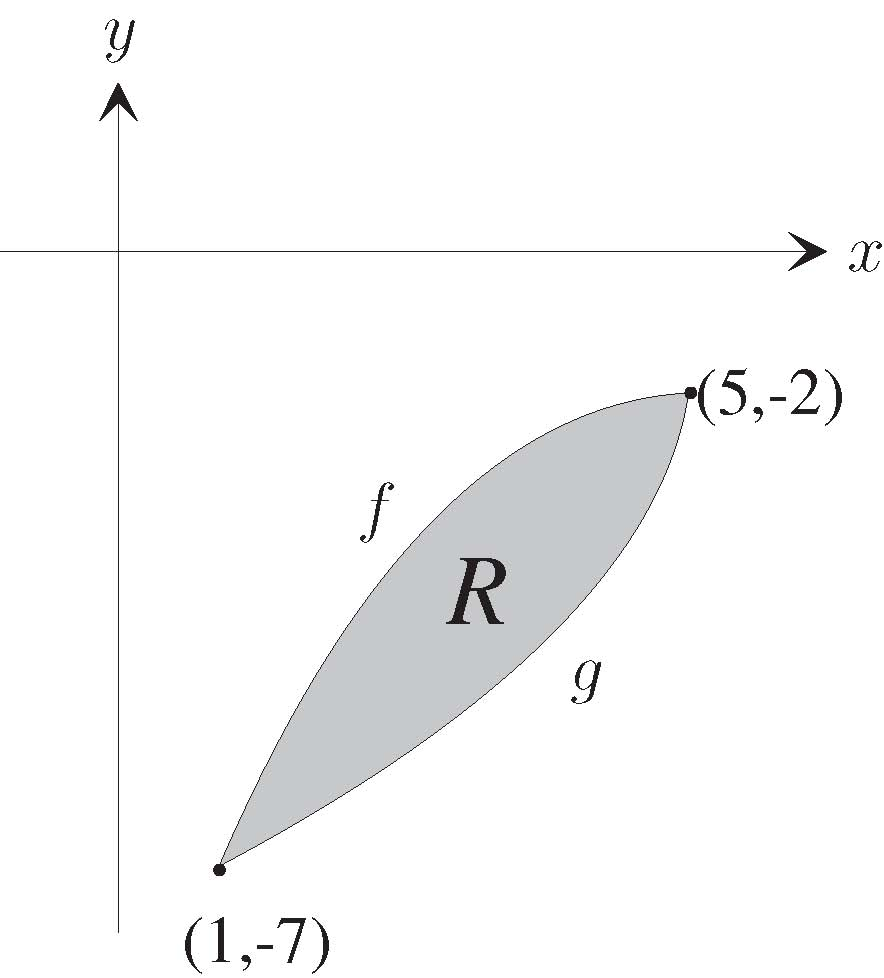
\includegraphics[scale=.2]{fig1}
\end{panel}
\begin{solution}
This a really good  solution. I hope this solution is correct or I
will be totally embarrassed to no end. Even if it is wrong, maybe
the students will appreciate my tremendous effort. You can see
from the figure that the solution is obvious.
\end{solution}
\end{splitsolution}
\end{problem}
\end{Verbatim}
Note the use of \cs{relax} in line~(4). The first object in the panel
environment is a command. To prevent the command from expanding
prematurely, place a \cs{relax} as above. This will give you the default
parameter of \texttt{r} and prevent expansion. The use of \cs{relax} is
only needed when there is a command immediately following the opening of
the \texttt{panel} environment; otherwise, just \verb!\begin{panel}! should
work correctly. The optional argument can always be specified,
\verb!\begin{panel}[r]!; this too would prevent the premature expansion of
any command that immediately follows.

The \texttt{panel} environment takes its contents and writes it verbatim
to a \textsf{CUT} file, then inputs it back in (at the end of the \texttt{panel}
environment), and places its contents in the box \cs{eqpanelbox} where it
takes it measurements of \cs{panelwidth} and \cs{panelheight} (the total
height).

The \texttt{splitsolution} environment \emph{must} enclose two
other environments: The \texttt{panel} and the \texttt{solutions}
environments, \emph{in that order}.

The \texttt{panel} environment comes first and takes optional argument.
The optional parameter has takes a value of `\texttt{r}' (the default) or
`\texttt{l}'. The \texttt{r} (resp., \texttt{l}) option means the panel is
to appear on the right (resp., left) of the solution (or vertical white
space).

After the \texttt{panel} environment comes the \texttt{solutions}
environment. The optional parameter of this environment need not
be specified, as it gets its value from the \texttt{split\-solution}
parameter.

There is a small gap of \texttt{3pt} (the default) inserted between the
panel and the solution. The value of this gap is contained in the
\cs{panelgap} command,
\begin{Verbatim}[xleftmargin=\amtIndent]
\newcommand\panelgap{3pt}
\end{Verbatim}
which can be redefined.

\redpoint The depth (the default is \cs{panelheight}) that you specify as
the parameter of the \texttt{splitsolution} environment needs to be large
enough to accommodate your typeset solution; otherwise, the solution will
overlap the next problem. This is because, unlike the solutions inside a
\texttt{solution} environment (but not in a \texttt{splitsolution}
environment) are typeset in a \texttt{minipage} with a specified depth.

To extend the height of the solution, use the following method.
\begin{Verbatim}[xleftmargin=\amtIndent]
\begin{splitsolution}[\panelheight+1in]
...
\end{splitsolution}
\end{Verbatim}
This sets the total height to be the natural height of the panel plus 1 inch.

\section{\textsf{eqexam} Options}\label{eqoptions}

The options documented here are entered as optional arguments of the eqexam package:
\begin{Verbatim}[xleftmargin=\amtIndent,commandchars=!()]
\usepackage[!meta(optionals)]{eqexam}
\end{Verbatim}
The optional arguments can also be introduced through \texttt{exambuilder.cfg}, the configuration file.
Create a text file with the name of \texttt{exambuilder.cfg}
and create the line shown below.
\begin{Verbatim}[xleftmargin=\amtIndent,commandchars=!()]
\ExecuteOptionsX{!meta(optionals)}
\end{Verbatim}
Place \texttt{exambuilder.cfg} in the folder of the source file and not on the {\LaTeX}
search path.

\redpoint The \textsf{eqexam} package has numerous options, some
inherited from \textsf{web}, some from \textsf{exerquiz}, and a
number of new ones.
\begin{description}
    \item[\texttt{forpaper}] Take this option when you want to create
        a black and white paper version of your test.

    \item[\texttt{forcolorpaper}] Take this option
        when you want to have a nice colorful paper version,
        or are publishing on the web in {\PDF}. See \Nameref{customColor}.

    \item[\texttt{nosolutions}] This is the normal option taken when
        you are printing a test for distribution to a class of
        students. When this option is taken, vertical space is
        generated by the \texttt{solutions} environment based on
        the value of its optional parameter. This leaves room for
        the student to solve/answer the question.

    \item[\texttt{nohiddensolutions}] If you use the \texttt{h}
        optional parameter for \texttt{problem} or \cs{item}, the
        solution will not be listed (at the end of the document)
        \emph{when you do not specify} \texttt{nosolutions}; but
        solutions will be typeset for the \texttt{solutionsafter} option.
        This option will override this feature.

    \item[\texttt{noHiddensolutions}] Normally, when you use the
    \texttt{H} optional parameter for \texttt{problem} or \cs{item}, the
    solution will not be listed when you use the \texttt{nosolutions} or
    \texttt{so\-lu\-tions\-af\-ter} options for \textsf{eqexam}. This option will
    override this feature.

    \item[\texttt{solutionsafter}] Causes solutions to appear
    following the statement of the problem.

    When the \texttt{solutionsafter} is in effect, the word
    \textit{Solution:} is typeset at the beginning of the solutions.
    The command \cs{renameSolnAfterTo} can be used for conveniently
    changing the \texttt{solutionsafter} label, for example, executing
    the command \verb!\renameSolnAfterTo{\textbf{Proof:}}! prior to a
    \texttt{solution} environment changes the label to
    \textbf{Proof:}; \verb!\renameSolnAfterTo{}! produces no
    label. These changes will be local to the group in which they are
    made, or global of there they are not made in a group.

    The command \cs{resetSolnAfterToDefault} sets the label text back to
    the default. The default label is \verb!\textit{Solution}:!.

    \item[\texttt{preview}] The bounding boxes are shown when this
    option is taken, provided the \texttt{online} or \texttt{email}
    option is chosen. See the description of these two options
    below.

    \item[\texttt{proofing}] Using this option will cause the
    correct answer for multiple choice questions to be marked with
    a check mark; the correct answers for fill-in questions
    (\cs{fillin} or \cs{TF}) are also shown.\medskip

    The \texttt{answerkey} option, described below,
    executes the \texttt{proofing} and \texttt{solutions\-after}
    options.

\end{description}

\redpoint The following options are unique to the \textsf{eqexam} package.

\begin{description}
\item[\texttt{pointsonleft}] The points for the problem are displayed in
    the left margin.

\item[\texttt{pointsonright}] The points for the problem are on the left
    margin.

\item[\texttt{pointsonboth}] Points are displayed in both margins.

\item[\texttt{nopoints}] Causes points not to be displayed, or
    calculated. Useful for writing documents that do not have points,
    such as a questionnaire.

\item[\texttt{totalsonleft}] The totals for each page can be
    displayed at the bottom left corner of each page using this option.

\item[\texttt{totalsonright}] The totals for each page can be
    displayed at the bottom right corner of each page using this
    option.

\item[\texttt{nototals}] Use this option if you don't want any
    totals at the bottom of the page.

\item[\texttt{noparttotals}] When multiple \texttt{exam} environments appear on
    the same page, they are separated by a horizontal rule. The page total
    for the closing \texttt{exam} environment is inserted into the margin on
    the same line as the horizontal rule. This option turns off the insertion
    of the page total for the closing \texttt{exam} environment.\medskip

    There are two commands that can be used for local control of
    this feature, they are \cs{eoeTotalOff} and \cs{eoeTotalOn}.
    When an \texttt{exam} ends near the bottom of one page, the
    new exam will begin on the next page, this results in the
    horizontal rule being generated with the end of exam totals,
    and the totals at the bottom as well. If these two numbers are
    the same, then you can turn off the end of exam total using
    \cs{eoeTotalOff}. Use this command just above
    \verb+\end{exam}+ and the changes will be local to that exam
    part.

\item[\texttt{parttotalsonright}] Place the part totals in the right
    margin, this is the default.

\item[\texttt{parttotalsonleft}] Place the part totals in the left
    margin.

\item[\texttt{nosummarytotals}] When you use the
    \texttt{instructions} environment, the total points for
    \texttt{exam} are displayed following the instruction heading.
    Using this option turns off this feature.

\item[\texttt{noseparationrule}] When the document has multiple
    \texttt{exam} environments, a separation rule is placed between
    them. This option turns off that feature.

    The design of the separation rule may be modified by the document author
    by redefining \cs{separationrule}, its definition is given below:
\begin{Verbatim}[xleftmargin=\amtIndent]
\newcommand{\separationrule}{\makebox[\linewidth]%
{\centering\rule{.67\linewidth}{.4pt}}}
\end{Verbatim}

\item[\texttt{coverpage}] Some instructors like to have a cover
    page for their exams, use this option to create a cover page. Use
    the \cs{eqexcoverpagedesign} command to design your own cover page.

\item[\texttt{coverpagesumry}] is a companion to the \texttt{coverpage} option,
    \texttt{coverpagesumry} takes one of three values: \texttt{bypages}, \texttt{byparts}, \texttt{none}.

\begin{description}
    \item[\texttt{coverpagesumry=bypages}] If \texttt{bypages} is chosen, an ``Exam Record''
    appears on the cover page. See the left-hand figure in
    Figure~\ref{fig:ExamRecord}. A page total appears on each line. Note
    ``Page~3,'' in the figure; the total there is ``$37\,\text{pts}\
    (12\,\text{pts}+25\,\text{pts})$.'' This means that there are 37
    points on page~3; on this page the first \texttt{exam} environment
    ended and a second \texttt{exam} environment begins, there are 12
    points on page~3 from the first \texttt{exam} environment, and 25
    points on that page from the second \texttt{exam} environment.

\begin{figure}[htb]
\begin{center}
\includegraphics[width=.4\linewidth]{bypages}\quad
\includegraphics[width=.4\linewidth]{byparts}
\caption{Exam Record}\label{fig:ExamRecord}
\end{center}
\end{figure}

    \item [\texttt{coverpagesumry=byparts}] If \texttt{byparts} is chosen, an
    ``Exam Record'' appears on the cover page that lists the number of
    points per part. (Each exam environment is considered here a
    ``part.'')  See the right-hand figure in
    Figure~\ref{fig:ExamRecord}.

    \item [\texttt{coverpagesumry=none}] If this option is chosen (the default), no
    ``Exam Record'' is generated. If the key \texttt{coverpagesumry} does not
    appear in the option list of \textsf{eqexam}, no ``Exam Record'' is written.

    \end{description}

    See \Nameref{examrecord} for more details on this topic.

\item[\texttt{nospacetowork}] When the \texttt{nosolutions} option
    is taken,  the \texttt{solutions}
    environment leaves vertical space in which to respond to the
    question. Use this option to override this behavior.\medskip

    The command \cs{SpaceToWork} causes the white space to be
    created again, and the \cs{NoSpaceToWork} turns it off again.
    Use these two commands to turn on and off the creation of
    vertical spaces in different parts of your exam.

\item[\texttt{answerkey}] This is a convenience option equivalent
    to \texttt{proofing} and \texttt{solutionsafter}. Useful for
    creating an ``answer key'' with answers and solutions displayed.

\item[\texttt{solutionsonly}] Using this option, it is possible to obtain
a typeset document consisting of only the solutions to \textsf{eqexam} document.
See \Nameref{solutionsonly} for further details.

\item[\texttt{vspacewithsolns}] An unusual feature requested by a user
    for homework assignments. This option is a combination of
    \texttt{nosolutions} (where vertical space is left by the
    \texttt{solutions} environment to respond to the question), but
    the solutions are written the \cs{jobname.sol} and input back in
    at the end of the document.

    This option is incompatible with \texttt{answerkey},
    \texttt{nosolutions}, and \texttt{solutionsafter}, so when
    \texttt{vspacewithsolns} is used, it ``cancels'' these other
    options.

    The command \cs{showAllAnsAtEnd} is inserted at the top of the
    \cs{jobname.sol} file and when \cs{jobname.sol} are input back
    in, the command \cs{showAllAnsAtEnd} is executed. The definition
    of \cs{showAllAnsAtEnd} is
\begin{Verbatim}[xleftmargin=\amtIndent]
\newcommand{\showAllAnsAtEnd}{%
    \makeAnsEnvForSolnsAtEnd
    \answerkeytrue\eq@proofingtrue
    \eq@solutionsaftertrue\vspacewithsolnstrue
    \displayworkareafalse\withsoldoctrue
}
\end{Verbatim}
Basically, this turns on all the switches that correspond to the
\texttt{answerkey} option. This command may be redefined to suite your
purposes.

\handpoint When this option is taken, the switch \cs{ifvspacewithsolns}
may be used to bring in alternate content.

See \Nameref{vspacewithsolns} for further details.

\item[\texttt{ftbsolns}] An alias for \texttt{vspacewithsolns}.

\item[\texttt{useforms}] Multiple choice questions have two forms,
    (1) the choices are labeled using letters (a), (b), (c), etc.; or
    (2) using a rectangular fill box. The default is~(1). The
    \texttt{useforms} switches the default to~(2). You can use the
    commands \cs{sqLinks} and \cs{sqForms} to change back and forth
    between these two types within the exam document. Using one of
    these commands outside a \texttt{problem} environment will
    globally change the default, from within, it will only change the
    default locally.

\item[\texttt{flextended}] When this option is taken, additional code is
    input to support filler lines, refer to Section~\ref{ss:VSFT} for
    details; in particular, read \Nameref{sss:flxtnd}.

\item[\texttt{myconfig}] If this option is taken, \textsf{eqexam}
    looks for the configuration file \texttt{eqexam.cfg}. This
    configuration file is input at the end of the package, and can be used
    to redefine, for language localization purposes, any of the (text)
    macros described in this manual. See the section \Nameref{custom} for
    a partial listing of macros that can be redefined and placed in
    \texttt{eqexam.cfg}.\medskip

\item[\texttt{myconfigi}\dots\texttt{myconfigvi}] Six additional
    options for inputting a configuration file. If you take one of
    these options, \textsf{eqexam} inputs the corresponding
    configuration file \texttt{eqexami.cfg}\dots\texttt{eqexamvi.cfg}.

\item[\texttt{cfg}] Syntax: \texttt{cfg=\anglemeta{basename}}. If this option is taken,
\textsf{eqexam} looks for a file named \texttt{\anglemeta{basename}.cfg} and is input.

    For one of my recent classes, I wrote many
    standard handouts documents: first day handout, assignment documents,
    homework assignments, review documents, test documents, and
    in-class notes. Each document-type had its own \textsf{eqexam}
    format (configuration file, \texttt{eqexami.cfg}\dots\texttt{eqexamiv.cfg}.
    It got confusing to keep track of all these configuration files. At which point
    I decided to add a \emph{named} configuration scheme. If you use the key \texttt{cfg}
    in the option list \texttt{cfg=firstday}, \textsf{eqexam} will look for a file
    named \texttt{firstday.cfg}

\item[\texttt{obeylocalversions}] An option put in to give greater control over
    versions.  Perhaps you have a \textsf{eqexam} file that has questions
    with multiple versions. You would like to pick and choose the versions
    to be used.  In this case, using \texttt{obeylocalversions} will cause
    \textsf{eqexam} to obey any \cs{selectVersion} commands embedded in
    the document.

\item[\texttt{allowrandomize}] Use this option to randomize
    the multiple choice/selection questions. See \Nameref{s:random} for details.

\item[\texttt{showgrayletters}] When \texttt{showgrayletters} is used, multiple choice
questions will have a gray capital letter
\texttt{A}, \texttt{B}, \texttt{C}, etc. underneath it. This letter
can then be referred to in the text or the solution using the \cs{REF} command.

See \Nameref{showgraylettersOpt} for more information.

    \item[\texttt{usexkv}] When this option is used, and the document
    author has the \textsf{xkeyval} package on his/her system, there is a
    re-definition of the \cs{fillin} command. For more information,
    see \Nameref{extendfillin}.

    \item[\texttt{allowcirc4mc}] Allows to use of circles (created by
    the \texttt{lcircle10} font) for multiple choice questions. See
    \Nameref{allowcirc4mc} for details.


\end{description}

\redpoint The next option concerns a major new feature, available
in \textsf{eqexam}, version 3.0 or later.

\begin{description}
    \item[\texttt{fortextbook}]\label{fortextbook} This option is designed support
        textbook authors. See \mlNameref{ftbop} for a greater explanation.
\end{description}

\redpoint The next two apply to files that have several versions in them,
these were defined for use by the \textsf{AeB Exam Builder}
utility,\footnote{\url{http://www.acrotex.net/builders/}} but they are
available to the document author.

\begin{description}
  \item[\texttt{max}] The value of \texttt{max}, \texttt{max=\anglemeta{N}},
  is a positive integer. The value of \texttt{max} is the
  number of versions for this document. This option executes
  \cs{numVersions\darg{\anglemeta{N}}} at the end of the package.

  \item[\texttt{rendition}] This is a key-value pair.
  \texttt{rendition=\anglemeta{alpha}}, where \anglemeta{alpha} letter corresponding to
  the version that is to be typeset. At the end of the package, the
  command \cs{forVersion\darg{\anglemeta{alpha}}} is executed.

\end{description}

\redpoint The next four options require the {\cAcroB}, and all of
its required packages, such as \textsf{hyperref}, their use
implies you are going to publish the document as a {\PDF}.

\begin{description}

\item[\texttt{pdf}] This option doesn't do much, it brings in the
    \textsf{web} package, which in turn, places the values of the
    keywords (\cs{title}, \cs{author}, \cs{subject}, etc.) into the
    Document Description dialog of the {\PDF}.

\item[\texttt{links}] This option brings in both \texttt{web} and
    \texttt{exerquiz}. When you do not use a solutions option
    (\texttt{nosolutions} and \texttt{solutionafter}), the solutions
    appear at the end of the document. When the \texttt{links} option
    is used, links from the questions to the solutions are created.
    Unless you use a ``paper option'' (\texttt{forpaper} and
    \texttt{forcolorpaper}), each solution is on a different page,
    making a document with a lot of pages. When you also specify a
    paper option, the solutions are separated by a \cs{medskip}.

\item[\texttt{online}] The \texttt{online} option implies the
    previous two options, but does more. When this option is taken,
    and the \texttt{nosolutions} option is specified, {\PDF} forms are
    created: multiple choice questions become radio button fields;
    fill-in questions become text fields, and the vertical space
    created by the \texttt{solutions} environment become multi-line
    text fields.\medskip

    This may be a useful option for an exam taken in a
    CBT\footnote{Computer Based Testing} lab, where the students
    can type in their responses and when finished, print the
    document to a lab printer to hand in.

\item[\texttt{email}] This option implies the \texttt{online}
    option, in addition, adds a submit button to the upper left corner
    of the first page of the exam. The student can take the test in a
    CBT lab, then submit the results to the instructor via email.

\end{description}
\noindent See the section \Nameref{email} for additional details
of these last two options.

\redpoint When any one of the four options above are taken, a
driver needs to be specified as well, the choices are\dots

\begin{description}

\item[\texttt{dvips}] For users of \textsf{dvips}, the
    dvi-to-postscript converter.

% \item[\texttt{pdftex}] For users of \textsf{pdftex} application.

% \item[\texttt{dvipdfm}] For users of \textsf{dvipdfm} application.

\item[\texttt{dvipsone}] For users of the
    {Y\!{\footnotesize\&}\!Y\TeX} System, such as myself.

%\item[\texttt{textures}] For \textsf{textures} users. (This
%  option is totally untested.)
\end{description}
The drivers \app{pdftex}, \app{luatex}, and \app{xetex} are automatically detected and need not
be specified as a driver option.

The driver names are passed on to \pkg{hyperref} and to
\pkg{eforms}\footnote{A component of \AcroB.} for the proper creation of
links and form fields.

\subsection{Configuration Files}

The \textsf{eqexam} looks for two configuration files, they are
\texttt{web.cfg} and \texttt{eqexam.cfg}.

The first one \texttt{web.cfg} may be already present on your hard
drive if you use the {\AcroB}. Typically, desired default driver
option is placed in here, for example, \texttt{web.cfg} might
contain the single line,
\begin{Verbatim}[xleftmargin=\amtIndent]
\ExecuteOptions{dvips}
\end{Verbatim}
\noindent for users of the \textsf{dvips} application for
converting \texttt{.dvi} files to \texttt{.ps} file. The drivers
supported by \textsf{eqexam} are listed in the previous section.

The second configuration file, \texttt{eqexam.cfg}, is input at
the end of the package, provided the document author takes the
\texttt{myconfig} option. Use this file to redefine some of the
commands described in \Nameref{custom}, and elsewhere, to
customize \textsf{eqexam}. An obvious use for this is to have a
language customization of the package, input through
\texttt{eqexam.cfg}.

If you place \texttt{eqexam.cfg} in the {\LaTeX} search path,
these customization will be global to all documents that specify
the \texttt{myconfig} option. If is is placed in the source
document folder (which is not in the {\LaTeX} search path) the
changes are local to all documents developed in that folder.

\subsection{The \texttt{solutionsonly} Option}\label{solutionsonly}

With this option, it is possible to obtain a listing of only the solutions
in an \textsf{eqexam} source file. A possible application of this feature
is if you publish homework or practice test questions, you can later
publish the solutions to them.

%\handpoint The demo file for this option is \texttt{eqex\_solnsonly.tex}, where you
%will find detailed instructions for how to do this. See also the file
%\texttt{text03.tex}, which demos both the \texttt{solutionsonly} option and the
%\texttt{vspacewithsolns} option.

\exAeBBlogPDF{p=1227} The demo file for this option is
\texttt{\href{\urlAcroTeXBlog/?p=1227}{eqex\_solnsonly.pdf}}, available from
the {\AcroBlog} website. The source file is attached to the PDF. Within the
source file, you will find detailed instructions for how to create a
solutions-only file.


\subsection{The \texttt{vspacewithsolns} Option}\label{vspacewithsolns}

With option is a combination of \texttt{nosolutions} (where vertical
spaces are left for extended response questions, and multiple choice and
fill-in the blank are left, well, blank) and compiling the document
with no options at all, in this case the solutions appear at the end of
the document.

To summarize, when \texttt{vspacewithsolns} is used, the test section is
left blank for the student to fill in, but at the end of the document are
the solutions. I've recently used this option to compile an old test (from
a previous semester) and publish it on the web. The student can try
solving the old test, with the solutions at the end of the
document.\footnote{Another option is to first publish your old exam with
the \texttt{nosolutions} option, then, after a suitable time, publish the same document
with the \texttt{solutionsonly} option.}

\newtopic An alias for this option is the option \texttt{ftbsolns}.

\exAeBBlogPDF{p=1220} The demo file for this feature is named
\texttt{\href{\urlAcroTeXBlog/?p=1220}{hw02.pdf}}. See also the file
\texttt{\href{\urlAcroTeXBlog/?p=1206}{test03.pdf}}, which demos both the
\texttt{solutionsonly} option and the \texttt{vspacewithsolns} option.

\subsection{The \texttt{fortextbook} Option and \textsf{fortextbook} Package}\label{ftbop}

This option is designed for authors of textbooks. The \texttt{fortextbook}
option defines the \texttt{probset} environment---used to create problems
sets in the textbook---as a re-purposing of the \texttt{exam}
environment. When the text is compiled with the \texttt{studented} option
(student edition), only odd-numbered solutions/answers are written to the
end of the document; when the \texttt{instred} option (instructor edition) is
used, all solutions/answers are written to the end of the document, there
are options for annotating the book with the answers in the margins or
following the questions (instructor edition).

Documentation for this option is found in the \texttt{doc/fortextbook}
folder. See the file \texttt{fortextbook.pdf} and its source file
\texttt{fortextbook.ltx}.

To use the \texttt{fortextbook} option, a whole panoply of options are needed,
\begin{Verbatim}[xleftmargin=\amtIndent]
\usepackage[%
    fortextbook,ftbsolns,usecustomdesign,
    forcolorpaper,noseparationrule,usexkv
]{eqexam}
\end{Verbatim}
Accompanying the \textsf{eqexam} is a simple wrapper package called
\texttt{fortextbook}, which basically calls \textsf{eqexam} with all the above
options. So, the textbook author needs only to specify,

\begin{Verbatim}[xleftmargin=\amtIndent]
\usepackage{fortextbook}
\end{Verbatim}
The documentation for this option is quite extensive and is
available in the separate document \texttt{fortextbook.pdf}. This
document is a short ``textbook'' that illustrates and documents
the features of this option.

See the \textbf{\ulSetLink{http://www.acrotex.net/blog}{Acro\TeX{}
Blog}} for several articles on the \texttt{fortextbook} option,
beginning with the first article
\textsl{\ulSetLink{http://www.acrotex.net/blog/?p=604}{The
\texttt{fortextbook} option, Part 1, The Instructor Edition}}. A
listing of all articles of the
\ulSetLink{http://www.math.uakron.edu/~dpstory/eqexam.html}{\textsf{eqexam}
package} may be obtained by following
\ulSetLink{http://www.acrotex.net/blog/?tag=eqexam-package}{this
link}.

The full series of articles on the \texttt{fortextbook} option may be found under the
\ulSetLink{http://www.acrotex.net/blog/?tag=fortextbook}{fortextbook tag} at the blog site.



\section{The \texttt{online} and \texttt{email} Options}\label{email}

When you use the \texttt{online} option, all fields created by the
\cs{fillin} command, and this includes \cs{TF}, are converted into
text fields, and the white space created by the \texttt{solutions}
environment is converted to a multi-line text field. The fields
manifest themselves when the document is viewed within the Adobe
Reader, or any other {\PDF} viewer that supports form fields.

This may be a useful option to the few people out there who are
not in a technical field that requires specialized symbols to
respond to a question. An exam created by the \texttt{online}
option can be filled out online, printed, and submitted to the
course instructor, perhaps within a lab setting.

There are other applications, such as creating a course survey, or
a questionnaire of some type the students can fill out and submit.
The \texttt{email} option may be more appropriate for these
applications.

\subsection{The \texttt{email} Option}

When you pass the \texttt{email} option to \textsf{eqexam}, this
does everything the \texttt{online} option does, in addition, it
creates a ``Submit'' button that appears in the top-left margin of
the exam (it does not appear on the cover page), and is placed
there by the \cs{maketitle} command, that normally goes just after
the opening of the document environment, \verb+\begin{document}+.

The forms button is all setup to submit to the server-side script,
\textsf{eqAttach.asp}, an active server page using
\textsf{vbscript} as its scripting language. This script, when
properly installed and functional, receives the form data
generated by the document and attaches it to an email, which it
sends off to the designated destination. Before discussing how to
install and use \textsf{eqAttach.asp}, let me cover some commands
that controls this button as well as options for changing what is
sent to the server-side script.

When you take the \texttt{email} option, you need to supply a
minimum of two pieces of information: the path to the server-side
script \textsf{eqAttach.asp} and the email address of the person
the results are to be sent. The command \cs{SubmitInfo} is used to
supply this info, for example,
\begin{Verbatim}[xleftmargin=\amtIndent]
\SubmitInfo{http://localhost/scripts}{dpstory@uakron.edu}
\end{Verbatim}
This command takes two arguments, the first is the URL to the
server-side folder that contains \textsf{eqAttach.asp}, the second
argument is the email address of the recipient of the email. (You
can have multiple recipients by separating the address by an
comma.)

After the student submits the responses to the questions, an email
is sent to the recipient (the instructor, perhaps). When the
recipient receives the email, s/he can save the {\FDF} attached file
(containing the student responses) to a folder on the local hard
drive. At least for a Windows machine when you open the {\FDF}, the
{\PDF} will be fetched and the student data will be populated into
the form fields.

Once this is done, the instructor can either save the populated
file to the hard drive for later processing (the Acrobat
application needed for this step) or print it to a printer for
grading by hand.

If the instructor has Acrobat, s/he can use the markup capability
of Acrobat to grade the electronic version of the test, and return
the electronic version, with markup, to the student.

Below is the subject and message body of a ``typical'' submittal for the
student ``John Q. Student''.

\begin{flushleft}
Message Subject:
\begin{Verbatim}[xleftmargin=\amtIndent]
Exam Results: Test 1 of U. S. History
\end{Verbatim}
\end{flushleft}

\begin{flushleft}
Message Body:
\begin{Verbatim}[xleftmargin=\amtIndent]
Exam Information:
    Course Name: U. S. History
    Exam: Test 1
    Student: John Q. Student
    TimeOfQuiz: 1/19/2005 12:07:56 PM
\end{Verbatim}
The {\FDF} is attached.
\end{flushleft}


\noindent The following commands can be used to modify the email message.

\redpoint\cs{EmailCourseName} is used to specify the name of the
course. The default value for this is \cs{websubject}, obtained
from the \cs{subject} macro used in the preamble; however, if you
want a different name in the email, perhaps with more information
included, you can redefine the value using this macro.
\begin{Verbatim}[xleftmargin=\amtIndent]
\EmailCourseName{\websubject} % the default
\end{Verbatim}

\noindent\textbf{\color{red}Important:} When you use {\TeX}
formatting in the subject, such as
\begin{Verbatim}[xleftmargin=\amtIndent]
\subject{\bfseries Calculus 1}
\end{Verbatim}
and you are using the \texttt{email} option, it will
be necessary to use \cs{EmailCourseName} to redefine the subject, e.g.,
\verb+\EmailCourseName{Calculus 1}+, to avoid possible {\TeX} compile
errors, or to prevent {\TeX} primitives being a part of your
email!

\redpoint\cs{EmailExamName} is used to specify the exam name of
the course. The default value for this is \cs{webtitle}, obtained
from the \cs{title} macro used in the preamble; however, if you
want a different name in the email, perhaps with more information
included, you can redefine the value using this macro.
\begin{Verbatim}[xleftmargin=\amtIndent]
\EmailExamName{\webtitle} % the default
\end{Verbatim}

\noindent\textbf{\color{red}Important:} If you use some {\TeX}
formatting in the title, such as
\begin{Verbatim}[xleftmargin=\amtIndent]
\title{\bfseries Test 1}
\end{Verbatim}
and you are using the \texttt{email} option, it will be necessary
to use \cs{EmailExamName} to redefine the title, e.g.,
\verb+\EmailExamName{Test 1}+, to avoid possible {\TeX} compile
errors, or to prevent {\TeX} primitives being a part of your
email!

\redpoint\cs{EmailSubject} The document author might want a custom
subject in the email, instead of the standard one. By using this
macro, he can design his own email subject.
\begin{Verbatim}[xleftmargin=\amtIndent]
\EmailSubject{} % the default
\end{Verbatim}
\noindent In this case \textsf{eqAttach.asp} inserts the standard one.
\begin{Verbatim}[xleftmargin=\amtIndent]
Exam Results: \webtitle of \websubject
\end{Verbatim}
\noindent The email would read ``\texttt{Exam Results: Test 1 of
Calculus I}'', for example.

To change the email subject we would put the following command in
the preamble:
\begin{Verbatim}[xleftmargin=\amtIndent]
\EmailSubject{Another Set of Cool Results}
\end{Verbatim}

\redpoint \cs{ServerRetnMsg} The server script
(\textsf{eqAttach.asp}) returns a message acknowledging the
receipt of the data, this command allows the document author to
customize the return message. The default definition is:
\begin{Verbatim}[xleftmargin=\amtIndent]
\ServerRetnMsg{}
\end{Verbatim}
\noindent In this case \textsf{eqAttach.asp} inserts the standard
one, ``Exam results successfully sent to your instructor!''.

To change the return message to something more meaningful, put
this command in the preamble, for example,
\begin{Verbatim}[xleftmargin=\amtIndent]
\ServerRetnMsg{Your responses to the \\TeX Survey have been
    received, thank you!}
\end{Verbatim}

\redpoint\cs{SubmitButtonLabel} is the label that appears on the
submit button.
\begin{Verbatim}[xleftmargin=\amtIndent]
\SubmitButtonLabel{Submit} % the default
\end{Verbatim}


\subsubsection{Installing \textsf{eqAttach.asp}}

On the server side, in order for \textsf{eqAttach.asp} to run
correctly, Microsoft Internet Information Server (IIS), version
4.0 or greater, is needed. The script \textsf{eqAttach.asp} needs
to be placed where ASP scripts have execute permissions.

The \textsf{eqAttach.asp} uses the \textsl{Acrobat FDF
Toolkit}\footnote{Currently located at the
\href{http://partners.adobe.com/public/developer/acrobat/devcenter.html}
{Acrobat Family Developer Center}.}, version 6.0. Follow the
directions for installation contained in the accompanying
documentation.

Install \textsf{eqAttach.asp} in a folder (perhaps called
\texttt{Scripts}) designated to execute scripts.  If you don't
have such a folder, then the  following steps explain how to
create a virtual directory through IIS that points to this folder.

\begin{enumerate}
\item Create a new folder on the system (\texttt{Scripts}, for
example). Its recommended location is inside the \texttt{Inetpub}
folder.

\item Place \textsf{eqAttach.asp} in this newly created folder.

\item In the MMC snap-in for IIS, create a virtual directory by
right-clicking on the Default Web Site and selecting \texttt{New >
Virtual Directory}.

\item Type ``Scripts'' (or whatever the name of the folder you
created in~Step~1) as the alias for the virtual directory, and
then link it to the physical directory you created in Step~1.

\item Make sure that ``Script execution'' privileges are enabled.
If not, enable them.
\end{enumerate}


\subsubsection{Setting up and Modifying the Script}

On the server side, in order for \textsf{eqAttach.asp} to run
correctly, Microsoft Internet Information Server (IIS), version
4.0 or greater, is needed. The script \textsf{eqAttach.asp} should
be placed where ASP scripts have execute permissions. There are
two methods of sending e-mail:
\begin{enumerate}
    \item \texttt{CDONTS}: This method (which is commented out by
        default) can be used on an NT server. Uncomment if you want to
        use CDONTS, and comment out the CDOSYS code lines that follow.
    \item \texttt{CDOSYS}: This can be run on a Win2000 or WinXP
        server.
\end{enumerate}

The script needs to be modified appropriate to your server, in
particular, search down in \texttt{eqAttach.asp} for the
configuration line
\begin{Verbatim}[xleftmargin=\amtIndent,fontsize=\fontsize{9}{11}\selectfont]
eqMail.Configuration.Fields.Item
    ("http://schemas.microsoft.com/cdo/configuration/smtpserver")
        = "mySMTP"
\end{Verbatim}
\noindent replace \texttt{mySMTP} with your SMTP server.

\subsubsection{Some Options}

The default behavior of \textsf{eqAttach.asp} is to return a
message to the document that indicates the receipt of the data,
this message is``Exam results successfully sent to your
instructor!'' The message, as explained earlier, can be changed
using the \cs{ServerRetnMsg}, like so
\begin{Verbatim}[xleftmargin=\amtIndent,fontsize=\fontsize{9}{11}\selectfont]
\ServerRetnMsg{Your TeX survey results have been received, thank you.}
\end{Verbatim}
\noindent Now, if for whatever reason you don't want this
confirmation message to return to the document for display in
alert box, you can sent the \texttt{silent} as part of the query
string. For example, if
\begin{Verbatim}[xleftmargin=\amtIndent,fontsize=\fontsize{9}{11}\selectfont]
\SubmitInfo{http://myWebSite/scripts/eqAttach.asp?silent\#FDF}
    {myname@mymailprovider}
\end{Verbatim}
\noindent placed in the preamble of your document specifies the
path to the script, silent mode, and the email address of the
recipient of the form data.

\medskip\noindent
Another other feature of \textsf{eqAttach.asp} that can be changed
through the query string is the \texttt{/F} key-value pair of the
\texttt{FDF} sent out in email. The value of this key is the path
to the document that sent the \texttt{FDF}, it may be a url (an
address on the Internet) or it could be a file specification of a
local hard drive. If you specify \texttt{nopath} in the query
string, like so
\begin{Verbatim}[xleftmargin=\amtIndent,fontsize=\fontsize{9}{11}\selectfont]
\SubmitInfo{http://myWebSite/scripts/eqAttach.asp?nopath\#FDF}
    {myname@mymailprovider}
\end{Verbatim}
\noindent then \textsf{eqAttach.asp} strips out the file path and
leaves only the file name.

\redpoint This is what I did with the \texttt{tex\_survey.tex}
source file. I placed \texttt{tex\_survey.pdf} in a \texttt{LaTeX
Survey} folder on my desktop. As the emails came in, I saved the
\textsf{FDF} attachments to this folder. By (double) clicking on
the \textsf{FDF}, \texttt{tex\_survey.pdf}, which is in the same
folder, opened and the form data populated the fields from whence
they were sent. It worked well for me.

If you don't use the \texttt{nopath} option, when you click
on an \texttt{FDF} file you've received by email, your browser
opens and the PDF on the Internet is brought into the
browser and the form data populates the form fields, \dots at least on
a Windows machine. \texttt{:-)}

\subsubsection{References}

The following links were used as a reference in the development of the
\texttt{Email.asp} script.
\begin{itemize}
    \item CDOSYS:
    \begin{itemize}
        \item \href{http://invisionportal.com/show_tutorial.asp?TutorialID=160}{Invision Portal}  Tutorial: CDOSYS email tutorial
        \item \href{http://msdn.microsoft.com/library/default.asp?url=/library/en-us/cdosys/html/_cdosys_imessage_interface.asp}
                {MSDN}: CDO for Windows 2000. The IMessage Interface. (Use MIE to view this page.)
        \item \href{http://www.asp101.com/articles/john/cdosmtprelay/default.asp}{ASP 101} Sending Email Via an External SMTP Server Using CDO
    \end{itemize}
    \item CDONTS
    \begin{itemize}
        \item \href{http://www.juicystudio.com/tutorial/asp/cdonts.html}{Juicy Studio} The ASP CDONTS Component
        \item \href{http://www.devasp.com/Samples/mail.asp}{DevASP} Sending Mail from ASP with CDONTS.NewMail Object
    \end{itemize}
\end{itemize}

\section{Bells, Whistles and other Customizations}

\subsection{Customizations}\label{custom}

We enumerate some commands for changing the default design of \textsf{eqexam}.

\subsubsection{Course Info Commands}\label{courseInfo}

\textsf{eqexam} has several commands for the student to provide some identification
information.

\redpoint \cs{eqexamName}. This command defines the macro
\cs{eq@ExamName} that creates the underlined space for the student
to enter his/her name, and also defines the text box form field,
in the case the \texttt{online} or \texttt{email} options are
taken. There are two (design) parameters for \cs{eqexamName}
\begin{Verbatim}[xleftmargin=\amtIndent,commandchars=!()]
\eqexamName[!meta(eforms_opts)]{!meta(width)}
\end{Verbatim}
\noindent The first optional parameter can be used to modify the
appearance of the text field, see the \href{eformman.pdf}{eForms}
documentation for details. The second parameter is the width of
the field. The default definition is
\begin{Verbatim}[xleftmargin=\amtIndent]
\eqexamName[\Ff\FfRequired]{2.25in}
\end{Verbatim}
\noindent Here, the text field that will be generated (when
\texttt{online} or \texttt{email} is specified) will be a required
field. The total width of the space provided is $2.25$ inches.

The command \cs{examNameLabel} controls the label to be used for
this name field. It takes one parameter, the label
to be used for the name field; the default definition is
\verb+\examNameLabel{Name:}+.

\redpoint \cs{eqSID}. This command defines the macro \cs{eq@SID}
that creates the underlined space for the student to enter his/her
student Identification number (SID), and also defines the text box
form field, in the case the \texttt{online} or \texttt{email}
options are taken. There are two (design) parameters for
\cs{eqSID}
\begin{Verbatim}[xleftmargin=\amtIndent,commandchars=!()]
\newcommand\eqSID[!meta(eforms_opts)]{!meta(width)}
\end{Verbatim}
\noindent The first optional parameter can be used to modify the
appearance of the text field, see the \href{eformman.pdf}{eForms}
documentation for details. The second parameter is the width of
the field. The default definition is
\begin{Verbatim}[xleftmargin=\amtIndent]
\eqSID[\Ff\FfRequired]{2.25in}
\end{Verbatim}
\noindent Here, the text field that will be generated (when
\texttt{online} or \texttt{email} is specified) will be a required
field. The total width of the space provided is $2.25$ inches.

The command \cs{examSIDLabel} controls the label used for this SID field.
It takes one parameter, the label to be used for the name field; the
default is \verb+\examSIDLabel{SID:}+.

\redpoint \cs{eqEmail}. This command defines the macro
\cs{eq@Email} that creates the underlined space for the student to
enter his/her student email address, and also defines the text box
form field, in the case the \texttt{online} or \texttt{email}
options are taken. There are two (design) parameters for
\cs{eqEmail}
\begin{Verbatim}[xleftmargin=\amtIndent,commandchars=!()]
\newcommand\eqEmail[!meta(eforms_opts)]{!meta(width)}
\end{Verbatim}
\noindent The first optional parameter can be used to modify the
appearance of the text field, see the \href{eformman.pdf}{eForms}
documentation for details. The second parameter is the width of
the field. The default definition is
\begin{Verbatim}[xleftmargin=\amtIndent,]
\eqEmail{2.25in}
\end{Verbatim}
\noindent Here, the text field that will be generated (when
\texttt{online} or \texttt{email} is specified). The total width
of the space provided is $2.25$ inches.


The command \cs{examEmailLabel} controls the label to be used for
this email field. It takes one parameter, the
label to be used for the name field; the default definition is
\verb+\examEmailLabel{Email:}+.


\subsubsection{Changing the Title and Cover Page}

\redpoint \cs{maketitle}. The main heading that appears at the top
of the first page of the exam is created by the {\LaTeX}
(redefined) command \cs{maketitle}. The \cs{maketitle} has some
code to place the email button in the top margin, followed by the
expansion of the command \cs{maketitledesign}, whose definition is
\begin{Verbatim}[xleftmargin=\amtIndent,fontsize=\fontsize{9}{11}\selectfont]
\newcommand\maketitledesign
{%
    \makebox[\textwidth]{\normalsize
        \shortstack[l]{\strut\websubject\\\@date}\hfill
        \shortstack[c]{\webtitle\\\strut\@altTitle}\hfill
        \shortstack[l]{\strut\eq@ExamName\\\webauthor}}%
}
\end{Verbatim}
This command can be redefined using \cs{renewcommand} to suite your needs, for example,
\begin{Verbatim}[xleftmargin=\amtIndent,fontsize=\fontsize{9}{11}\selectfont]
\makeatletter
\renewcommand\maketitledesign
{%
    \makebox[\textwidth]{\normalsize
        \shortstack[l]{\strut\websubject\\\webauthor, \@date}\hfill
        \shortstack[l]{\webtitle\\\strut\@altTitle}\hfill
        \shortstack[l]{\strut\eq@ExamName\\\eq@SID}}%
}
\makeatother
\end{Verbatim}
\noindent This code adds in a field for the student to enter
his/her student Id, here we enclose the code in a
\cs{makeatletter}/\cs{makeatother} because this redefinition
occurs in the preamble, and the code has an `\texttt{@}' in it.

Command elements that are appropriate to the redefinition are \cs{maketitledesign} are\dots
\begin{description}
    \item[\cs{websubject}] This is the course name, as determined by the \cs{subject} command.
    \item[\cs{webtitle}] This is the exam name as determined by the \cs{title} command.
    \item[\cs{altTitle}] An additional text field that is placed below \cs{webtitle}.
    \item[\cs{@date}] This is the date as determined by the \cs{date} command.
    \item[\cs{eq@ExamName}] This is the name field for the student to enter his/her name, as defined
        by default or redefined by \cs{eqexamName}, see \Nameref{courseInfo}.
    \item[\cs{eq@SID}] This is the student ID field for the student to enter his/her ID, as
        defined by default, or redefined by the command \cs{eqSID}, see \Nameref{courseInfo}.
    \item[\cs{eq@Email}] This is the student email field for the student to enter an email address, as
        defined by default, or redefined by \cs{eqEmail}, see \Nameref{courseInfo}.
    \item[\cs{theduedate}] This is a text macro defined by the \cs{duedate} command. For example, setting
    \verb+\duedate{03/10/05}+ defines \cs{theduedate} so that it expands to \texttt{03/10/05}. May
    be useful when redefining \cs{maketitledesign} for a homework assignment page.
\end{description}

\redpoint \cs{eqexcoverpagedesign}. When the \texttt{coverpage} option is
taken, a default cover page appears unless it is redefined. The
\textsf{eqexam} package provides \cs{eqexcoverpagedesign} to design your
own cover page. The default cover page uses the

\begin{description}
    \item[\cs{websubject}] This is the course name, as determined by the \cs{subject} command.
    \item[\cs{webtitle}] This is the exam name as determined by the \cs{title} command
    \item[\cs{webuniversity}] This is the value set by the \cs{university} command, given
        in the preamble.
    \item[\cs{@date}] This is the date as determined by the \cs{date} command.
    \item[\cs{eq@ExamName}] This is the name field for the student to enter his/her name, as defined
        by default or redefined by \cs{eqexamName}, see \Nameref{courseInfo}.
    \item[\cs{eq@SID}] This is the student ID field for the student to enter his/her ID, as
        defined by default, or redefined by the command \cs{eqSID}, see \Nameref{courseInfo}.
    \item[\cs{eq@Email}] This is the student email field for the student to enter his/her email address, as
        defined by default, or redefined by \cs{eqEmail}, see \mlNameref{courseInfo}.
\end{description}
Copy the definition of \cs{eqexcoverpagedesign} from
\textsf{eqexam.dtx} and modify as desired. Place the new
definition in the preamble (enclosed between
\cs{makeatletter} and \cs{makeatother}) or in a custom style file. No
special support for this design is offered, because a cover page
can be designed in so many different ways.

\newtopic Another command associated with the \texttt{coverpage} option,is the
\cs{place\-Cover\-Page\-Logo}, a simple command used to insert a logo on the cover page.
The logo can be used to cover the score in the next page if the
instructor places the score under the logo. Example of usage
\begin{Verbatim}[xleftmargin=\amtIndent,fontsize=\fontsize{9}{11}\selectfont]
\placeCoverPageLogo{5in}{-1.5in}{
\includegraphics{nwfsc_logo}}
\end{Verbatim}
Working from the upper left corner, the first parameter is the amount to move to logo
to the right, the second parameter is the amount to move the logo vertically. The
Third parameter is the content; perhaps an \cs{includegraphics} command.


\subsubsection{Changing the Running Headers}

There are two running headers, one header for the exam itself, and
another when the solutions are shown at the end of the document.

\redpoint Running Header for Exam. The commands \cs{lheadeqe},
\cs{cheadeqe} and \cs{rheadeqe} are used for defining the left, right, and
center running headers. \textbf{Note:} these commands have been recently
renamed, originally they were named \cs{lhead}, \cs{chead} and \cs{rhead},
but this conflicts with the \textsf{fancyhdr} package. If
\textsf{fancyhdr} has not been loaded by the time \textsf{eqexam} is
loaded, the eqexam definitions for \cs{lhead}, \cs{chead} and \cs{rhead}
still hold. Generally, it is recommended that the new command be used,
\cs{lheadeqe}, \cs{cheadeqe} and \cs{rheadeqe}.

\begin{enumerate}
\item \begin{Verbatim}[commandchars=!()]
\lheadeqe{!meta(text)}
\end{Verbatim}
Changes the left header text of the running header. This command defines an
internal macro \cs{eq@lhead} that actually contains the text. The default is
\begin{Verbatim}[xleftmargin=\amtIndent]
\lheadeqe{\shortwebsubject/\shortwebtitle}
\end{Verbatim}

\item \begin{Verbatim}[commandchars=!()]
\cheadeqe{!meta(text)}
\end{Verbatim}
Changes the center header text of the running header.
This command defines an internal macro \cs{eq@chead} that actually
contains the text. The default is
\begin{Verbatim}[xleftmargin=\amtIndent,fontsize=\fontsize{9}{11}\selectfont]
\cheadeqe{-- Page \arabic{page}\space of \nPagesOnExam\space--}
\end{Verbatim}

\item \begin{Verbatim}[commandchars=!()]
\rheadeqe{!meta(text)}
\end{Verbatim}
\noindent Changes the right header text of the running header.
This command defines an internal macro \cs{eq@rhead} that actually
contains the text.
\item[]The default is \verb+\rhead{\eq@ExamName}+.
\end{enumerate}
If you want to redesign the layout of the running
header, here is the macro that the above components fill.
\begin{Verbatim}[xleftmargin=\amtIndent,fontsize=\fontsize{9}{11}\selectfont]
\newcommand\runExamHeader{\eq@lhead\hfill\eq@chead\hfill\eq@rhead}
\end{Verbatim}

\redpoint Running Header for Solutions. The components of the
running header for the solutions pages occur, as above, on the left, center
and right of each header are defined by the commands \cs{lheadSol},
\cs{cheadSol} and \cs{rheadSol}.

\begin{enumerate}
\item \begin{Verbatim}[commandchars=!()]
\lheadSol{!meta(text)}
\end{Verbatim}
\noindent Changes the left header text of the running header. This
command defines an
internal macro \cs{eq@lheadSol} that actually contains the text. The default is
\begin{Verbatim}[xleftmargin=\amtIndent]
\lheadSol{\shortwebsubject/\shortwebtitle}
\end{Verbatim}


\item \begin{Verbatim}[commandchars=!()]
\cheadSol{!meta(text)}
\end{Verbatim}
\noindent Changes the center header text of the running header.
This command defines an internal macro \cs{eq@cheadSol} that
actually contains the text. The default is
\begin{Verbatim}[xleftmargin=\amtIndent,fontsize=\fontsize{9}{11}\selectfont]
\cheadSol{-- Page \arabic{page}\space of \nPagesOnExam\space--}
\end{Verbatim}

\item \begin{Verbatim}[commandchars=!()]
\rheadSol{!meta(text)}
\end{Verbatim}
\noindent Changes the right header text of the running header.
This command defines an internal macro \cs{eq@rheadSol} that
actually contains the text. The default definition is
\verb+\rheadSol{SOLUTIONS}+.
\end{enumerate}
\noindent If you want to redesign the layout of the running
header, here is the macro that the above components fill.
\begin{Verbatim}[xleftmargin=\amtIndent]
\newcommand\runExamHeaderSol
    {\eq@lheadSol\hfill\eq@cheadSol\hfill\eq@rheadSol}
\end{Verbatim}

\subsubsection{Changing the Running Footers}

The default set up of \textsf{eqexam} is to use no running footers;
actually, that's not quite right. \textsf{eqexam} places the command
\cs{settotalsbox} in the footer; this command is the one that places the
totals boxes, when requested.

\newtopic\textsf{eqexam} defines three commands for the footer,
\settowidth{\aebdimen}{\ttfamily\string\lfooteqe\darg{\meta{text}}}
\begin{dCmd}[commandchars=!()]{\aebdimen+2\fboxsep+2\fboxrule}
\lfooteqe{!meta(text)}
\cfooteqe{!meta(text)}
\rfooteqe{!meta(text)}
\end{dCmd}
\noindent where the \meta{text} is placed at the left, center, and
right of the running footer. The default for each is empty text. These
three comprise the definition of \cs{runExamFooter}
\begin{dCmd}{\linewidth}
\newcommand{\runExamFooter}{\eq@lfoot\hfill\eq@cfoot\hfill\eq@rfoot}
\end{dCmd}
\noindent The \cs{settotalsbox} and \cs{runExamFooter} then appear in the definition
of \cs{@oddfoot} in the definition of the \texttt{eqExamheadings} page style.
\begin{Verbatim}[xleftmargin=\amtIndent]
\renewcommand{\@oddfoot}{\settotalsbox\runExamFooter}
\end{Verbatim}
When doing any re-definition of the running footers at the \cs{@oddfoot} command,
be sure to include \cs{settotalsbox} on the \emph{left side of the running footer}; otherwise,
you will not have a totals box when you request one.


\subsubsection{Exam Strings}

In this section we list a new commands that contain information about the exam.

\settowidth{\aebdimen}{\ttfamily\string\nPagesOnExam}
\begin{dCmd}[commandchars=!()]{\aebdimen+2\fboxsep+2\fboxrule}
\nPagesOnExam
\end{dCmd}
\noindent The command \cs{nPagesOnExam} expands to the total number of pages in the exam.

\settowidth{\aebdimen}{\ttfamily\string\nQuesInExam\darg{\meta{exam\_name}}}
\begin{dCmd}[commandchars=!()]{\aebdimen+2\fboxsep+2\fboxrule}
\nQuesInExam[!meta(exam_name)]
\end{dCmd}
\noindent \cs{nQuesInExam} expands to the total number of questions in the
exam. The command takes an optional argument, the \meta{exam\_name}
(this is the name given the exam as the required argument of the
\texttt{exam} environment). If the argument is not given, the name of the
current exam is used (when executed within an \texttt{exam} environment).
If \cs{nQuesInExam} appears outside an \texttt{exam} environment, the value of
the optional argument needs to be specified.

\newtopic There are several commands are useful for documents that have several
\textsf{eqexam} environments, these are
\settowidth{\aebdimen}{\ttfamily\string\percentForPart\darg{\meta{exam\_name}}}
\begin{dCmd}[commandchars=!()]{\aebdimen+2\fboxsep+2\fboxrule}
\theGrandTotal
\totalForPart{!meta(exam_name)}
\percentForPart{!meta(exam_name)}
\end{dCmd}
\noindent The first command sums the point totals for each of the
\texttt{exam} environments. The latter two, each taking one argument, the
name associated with the \texttt{exam}, reports the points for that
\texttt{exam} environment and the percent of the total for that
\texttt{exam} environment.

\newtopic Below is a recent example taken from a final exam that I constructed for my class.
\begin{Verbatim}[xleftmargin=\amtIndent,fontsize=\small]
\begin{eqComments}[Final Exam:] (\theGrandTotal\space points) The
final exam has two parts:
    \textbf{Part I} (\totalForPart{InstrQuestions} points or
       \percentForPart{InstrQuestions} of the total points) consists of
       questions written by the instructor;
    \textbf{Part II} (\totalForPart{GenEd} points or
       \percentForPart{GenEd} of the total points) consists of
       questions provided by the Department of Mathematics.
\end{eqComments}
\end{Verbatim}

%\promoteNewPageHere{10pt}

\handpoint The calculation of \cs{percentForPart} is done in one of two ways:
\begin{enumerate}
 \item If the \textsf{fp} package is loaded, ``floating point
     arithmetic'' is used and results are rounded to the number of
     decimal points determined by \cs{nPctDecPts}, the default
     definition of which is \verb!\newcommand{\nPctDecPts}{1}!. This command may be redefined
     to another nonnegative integer value.
\item Otherwise---if the \textsf{fp} package is \emph{not
    loaded}---\TeX's count registers are used, the percentage rounded
    to the nearest integer.
\end{enumerate}

\newtopic The calculations are made when the \cs{maketitle} command is
expanded. If, for whatever reason, you are not using \cs{maketitle}, you
can place the command that does the calculations,
\cs{EQEcalculateAllTotals}, just after \verb!\begin{document}!, and before
the first use of \cs{theGrandTotal} and \cs{percentForPart}.

\settowidth{\aebdimen}{\ttfamily\string\firstPageOfExam\darg{\meta{exam\_name}}}
\begin{dCmd}[commandchars=!()]{\aebdimen+2\fboxsep+2\fboxrule}
\firstPageOfExam{!meta(exam_name)}
\lastPageOfExam{!meta(exam_name)}
\end{dCmd}
\noindent These two commands expand the page numbers of the beginning and the ending
of the exam environment, respectively, with name \meta{exam\_name}.

\subsubsection{Localization of Strings}

% Added 01/10/06
% \examNameLabel
% \ptsLabel, \ptsLabel
% \eachLabel
% \pointsLabel, \pointLabel
% \defaultInstructions

In this section we list various macros that expand to text
appearing on an \textsf{eqexam} document. The default text is in
English.  These commands can be redefined to other English
language phrases, or to other languages, and placed in the preamble of your document,
or in one of the \texttt{.cfg} files.

\begin{itemize}
% Added 01/10/06
\item\cs{examNameLabel}: On each page of the exam, there is a place
for the student to enter her/his name. \cs{examNameLabel} can be
used to define the name label, the default is
\begin{Verbatim}[xleftmargin=\amtIndent]
\examNameLabel{Name:}
\end{Verbatim}
\item \cs{examAnsKeyLabel}: When the \texttt{answerkey} option is in
    effect, the line in which the student enters her/his name (labeled by
    \cs{examNameLabel}) is filled by the value of the text macro
    \cs{examAnsKeyLabel}. The default definition is
\begin{Verbatim}[xleftmargin=\amtIndent]
\examAnsKeyLabel{Answer Key}
\end{Verbatim}
Thus, when the \texttt{answerkey}
option is used, the name field appears as follows:
\begin{flushleft}
\underbar{\makebox[2.5in][l]{Answer Key}}
\end{flushleft}

\item\cs{ptLabel} and \cs{ptsLabel}: Labels for indicating the points of a problem, the first is
the singular form of the second. The default is
\begin{Verbatim}[xleftmargin=\amtIndent]
\ptLabel{pt}            % singular form
\ptsLabel{pts}          % plural form
\end{Verbatim}
\item\cs{eachLabel}: Label for indicating the common point value of each of several parts
of the same problem.
\begin{Verbatim}[xleftmargin=\amtIndent]
\eachLabel{ea.}
\end{Verbatim}
\item\cs{pointLabel} and \cs{pointsLabel}: The word for `points' used in the \texttt{instructions} environment
    that lists the number of points in this exam. The default is
\begin{Verbatim}[xleftmargin=\amtIndent]
\pointLabel{point}      % singular form
\pointsLabel{points}    % plural form
\end{Verbatim}
The \cs{pointsLabel} command defines \cs{eq@pointsLabel}, which,
in turn, is used in the \cs{summaryTotalsTxt}, the definition of
which follows:
\begin{Verbatim}[xleftmargin=\amtIndent]
\newcommand{\summaryTotalsTxt}
    {($\summaryPointTotal\,\text{\eqpointsLabel}$)}
\end{Verbatim}
\item\cs{defaultInstructions}: The \texttt{instructions} environment has a default heading.
The command \cs{defaultInstructions} allows you to change this heading. The default is
\begin{Verbatim}[xleftmargin=\amtIndent]
\defaultInstructions{Instructions.}
\end{Verbatim}
\end{itemize}

\newtopic See \Nameref{ptTotalsBoxes} as well as the section \mlNameref{courseInfo} for
additional details on these and commands useful for laying out the
standard text of an \textsf{eqexam} document.

\subsubsection{Customization of Color}\label{customColor}

When the \texttt{forcolorpaper} option is used, various elements---such as
section titles, instruction headers, color for fill-in problems, and so on---have default colors. In
this section we list the color controls, along with their default definitions.

\begin{Verbatim}[numbers=left,xleftmargin=\amtIndent,fontsize=\fontsize{10}{14}\selectfont]
\proofingsymbolColor{red}
\instructionsColor{blue}
\eqCommentsColor{blue}
\eqCommentsColorBody{black}
\universityColor{blue}
\titleColor{black}
\authorColor{black}
\subjectColor{blue}
\linkcolor{blue}
\nolinkcolor{blue}
\fillinColor{red}
\forceNoColor
\end{Verbatim}

\noindent\textbf{Description of Color Commands:}
\begin{enumerate}
   \item The color of the proofing symbol, it appear for multiple
       choice questions with the \texttt{answerkey} option in effect.
   \item The color of the header text for the \texttt{instructions} environment.
   The header is the text that appears in the optional argument.
   \item The color for the header text for the \texttt{eqComments} environment.
   The header is the text that appears in the optional argument.
   \item The color for the body of the text for the \texttt{eqComments} environment.
   \item The color of the university, visible only when the \texttt{coverpage} option is taken.
   \item The color of the title, visible only when the \texttt{coverpage} option is taken.
   \item The color of the author, visible only when the \texttt{coverpage} option is taken.
   \item The color of the subject, visible only when the \texttt{coverpage} option is taken.
   \item The color applied to a link, applies only when \textsf{hyperref} is included through one of the PDF options,
         \texttt{links}, \texttt{online}, or \texttt{email}.
   \item The color applied to a link that has been turned off, applies
       only when \textsf{hyperref} is included through one of the PDF options,
       \texttt{links}, \texttt{online}, or \texttt{email}.
   \item The color of the a fill-in (including a True/False question)
       when one of the options \texttt{answerkey},
       \texttt{vspacewithsolns}, or \texttt{solutionsonly} is
       taken.
   \item This convenience command forces all the above colors to black. Useful when you want to use the
   \texttt{showgrayletters}. This produces a black and white document, with gray letters. (If you use the
   \texttt{forpaper} option, the gray letters appear black.)
\end{enumerate}


\subsection{Creating Multiple Versions of Exam}

Unfortunately, I teach multiple sections of the same course, and
am faced with the problem of writing different exams for the same
course each administered to a different section.

Typically, I only have a need for two variations on the test; however,
further extensions can be made, if needed (See \Nameref{mutiVerNew})

\subsubsection{The Original Version Scheme}\label{mutiVerOrig}

The \textsf{eqexam} package defines a boolean switch,
\cs{ifVersionA} for this purpose. The two sections of the same
course are ``Version A'' and ``Version B''. The default is that
you are preparing an exam for ``Version A''.

The command \cs{forVersion} sets the version: \verb+\forVersion A+
sets version to ``Version A'', and \verb+\forVersion B+ set the
version to ``Version B''. (The argument of the \cs{forVersion} command is case
insensitive, so you also type in \verb+\forVersion b+.)

For small variations in text, there is the \cs{ifAB} macro,
\settowidth{\aebdimen}{\ttfamily\string\ifAB\darg{\anglemeta{Version A text}}%
\darg{\anglemeta{Version B text}}}
\begin{dCmd}[commandchars=!()]{\aebdimen+2\fboxsep+2\fboxrule}
\ifAB{!anglemeta(Version A text)}{!anglemeta(Version B text)}
\end{dCmd}
\noindent for example, one could say,
\begin{Verbatim}[xleftmargin=\amtIndent]
\begin{problem}[2]
Compute $\frac{d}{dx}\ifAB{x^2}{x^3}$.
\end{problem}
\end{Verbatim}
\noindent For longer variations, the \texttt{comments} package is
used to create comment environments that are included or excluded.
The two environments are \texttt{verA} and \texttt{verB}.
\begin{Verbatim}[xleftmargin=\amtIndent]
\begin{problem}[2]
Compute $\frac{d}{dx}\ifAB{x^2}{x^3}$.

\begin{solution}[1in]
We use standard techniques:
\begin{verA}
$$
    \frac{d}{dx} x^2 = 2x
$$
\end{verA}
\begin{verB}
$$
    \frac{d}{dx} x^3 = 3x^2
$$
\end{verB}
\end{solution}
\end{problem}
\end{Verbatim}

There are several convenience macros for referring to the exams
generated by the two variations.

Usually, an exam, test, homework assignment has a number associate
with it, e.g. ``Exam 1'', ``Test 2'', ``Assignment~\#12'', etc\@.
This number should be defined using the \cs{examNum} macro.
\settowidth{\aebdimen}{\ttfamily\string\examNum\darg{\meta{num}}}
\begin{dCmd}[commandchars=!()]{\aebdimen+2\fboxsep+2\fboxrule}
\examNum{!meta(num)}
\end{dCmd}
where \meta{num} is the number to be associated
with the exam (test, assignment) under construction.

This command \emph{must appear before}  \cs{title} in the
preamble. The command \cs{examNum} takes its argument and defines
another macro \cs{nExam}, which has no arguments, but expands to
\meta{num}.

The \textsf{eqexam} package defines two commands \cs{Exam} and
\cs{sExam} to automatically enter the test information for the
current version. In the preamble, you can say,
\begin{Verbatim}[xleftmargin=\amtIndent]
\title[\sExam]{\Exam}
\end{Verbatim}
\noindent \cs{Exam} is the long version of the test name, and takes as its
argument the exam number. \cs{sExam} is the short version, having no
argument. Both \cs{Exam} and \cs{sExam} use the value determined by
\cs{examNum}, described above.

The text of \cs{Exam} and \cs{sExam} are generated by the four
commands,
\begin{enumerate}
\item \cs{VersionAtext\darg{\meta{text}}} This is the text for the long
version of the exam name for ``Version A''. The default text is
\begin{Verbatim}[xleftmargin=\amtIndent]
\VersionAtext{Exam~\nExam--Version A}
\end{Verbatim}

\item \cs{VersionBtext\darg{\meta{text}}} This is the text for the long
version of the exam name for ``Version B''. The default text is
\begin{Verbatim}[xleftmargin=\amtIndent]
\VersionAtext{Exam~\nExam--Version B}
\end{Verbatim}

\item \cs{shortVersionAtext\darg{\meta{text}}} This is the text for the
short version of the exam name for ``Version A''. The default text
is
\begin{Verbatim}[xleftmargin=\amtIndent]
\VersionAtext{Exam~\nExam A}
\end{Verbatim}

\item \cs{shortVersionBtext\darg{\meta{text}}} This is the text for the
short version of the exam name for ``Version B''. The default text
is
\begin{Verbatim}[xleftmargin=\amtIndent]
\VersionAtext{Exam~\nExam B}
\end{Verbatim}
\end{enumerate}

\redpoint All the above commands,
\textbf{\textcolor{blue}1}--\textbf{\textcolor{blue}4}, need to
appear before \cs{title} in the preamble.\medskip

\noindent Below is a ``typical'' example of how to correctly
redefine all the version text.
\begin{Verbatim}[xleftmargin=\amtIndent,fontsize=\fontsize{9}{11}\selectfont]
\documentclass{article}
\usepackage{amsmath}
\usepackage[forpaper,pointsonleft,noparttotals,nosolutions]{eqexam}

\examNum{1}
\forVersion{B}
\VersionAtext{Test~\nExam--003}
\VersionBtext{Test~\nExam--007}
\shortVersionAtext{T{\nExam}s3}
\shortVersionBtext{T{\nExam}s7}

\title[\sExam]{\Exam}
\author{D. P. Story}
\subject[C2]{Calculus II}
\date{Spring \the\year}
\keywords{Test \nExam, Section \ifAB{003}{007}}
\end{Verbatim}


\subsubsection{New Version Control}\label{mutiVerNew}

In this section we introduce a new set of commands that supersede
the commands defined above. Those commands were limited to only
two versions. The ones below can handle up to $26$ versions.

The steps for creating a multiple version \textsf{eqexam} document are as follows.
\settowidth{\aebdimen}{\ttfamily\string\numVersions\darg{\meta{num}}}
\begin{dCmd}[commandchars=!()]{\aebdimen+2\fboxsep+2\fboxrule}
\numVersions{!meta(num)}
\end{dCmd}
\noindent In the preamble, declare the number of versions for this document
 using \cs{numVersions}, e.g., \verb|\numVersions{3}|.
\begin{Verbatim}[xleftmargin=\amtIndent,commandchars=!()]
\longTitleText
    {!anglemeta(Text_1)}
    {!anglemeta(Text_2)}
    ...
    {!anglemeta(Text_n)}
\endlongTitleText
\end{Verbatim}
\begin{Verbatim}[xleftmargin=\amtIndent,commandchars=!()]
\shortTitleText
    {!anglemeta(Text_1)}
    {!anglemeta(Text_2)}
    ...
    {!anglemeta(Text_n)}
\endshortTitleText
\end{Verbatim}
\textbf{Note:} If there are more titles than what are declared, the rest
of the titles are absorbed (gobbled). If there are fewer titles than declared, a
{\LaTeX} package error is generated, and ``fake'' titles are
generated.


\newtopic Next, state the long and short titles for the document,
one for each of the declared number of versions given earlier in \cs{numVersions}.
For example, we can use the value \cs{nExam} in our titles. Usage:
\begin{Verbatim}[xleftmargin=\amtIndent]
\longTitleText
    {Test~\nExam--Version A}
    {Test~\nExam--Version B}
    {Test~\nExam--Make Up}
\endlongTitleText
\shortTitleText
    {T\nExam A}
    {T\nExam B}
    {T\nExam MU}
\endshortTitleText
\end{Verbatim}
These two commands give values to \cs{Exam} and \cs{sExam}. If
\verb!\forVersion{a}! is executed, \cs{Exam} expands to the text \verb|Test~\nExam--Version A| and
\cs{sExam} expands to \verb|T\nExam A|, using the example above. The value of \cs{nExam}
is determined by the \cs{examNum} command, as described above.

\newtopic Next is the command that does all the work. It creates alternate
text macros for each of the versions declared using \cs{numVersions}. The syntax is
\settowidth{\aebdimen}{\ttfamily\string\forVersion\darg{\meta{letter}}}
\begin{dCmd}[commandchars=!()]{\aebdimen+2\fboxsep+2\fboxrule}
\forVersion{!meta(letter)}
\end{dCmd}
For example, assuming \verb|\numVersions{3}|, \verb|\forVersion{a}| (or \verb|\forVersion{A}|) defines $3$ text commands \cs{vA}, \cs{vB} and
\cs{vC}, each taking one argument, the text you want to display:
\begin{Verbatim}[xleftmargin=\amtIndent]
 Name the \vA{place}\vB{date}\vC{year} of the signing
 of the Magna Carta.
\end{Verbatim}
\noindent Since \verb|forVersion{a}| was declared, only the \cs{vA} text
is displayed, the others are gobbled up. But wait, time out, the \cs{forVersion}
does more than that! It also creates a series of comment environments
\verb|\begin{verA}/\end{verA}|, \verb|\begin{verB}/\end{verB}|, \verb|\begin{verC}/\end{verC}|, etc.,
where only the version for which this compile applies will be typeset,
the others are commented out.
\begin{Verbatim}[xleftmargin=\amtIndent,fontsize=\fontsize{9}{11}\selectfont]
\numVersions{3}
\forVersion{b}
...
\begin{document}
...
Solve the equation for $\vA{x}\vB{y}\vC{z}$:
\[
\begin{verA}
       2x + 4 = 7
\end{verA}
\begin{verB}
       5y + 2 = 4
\end{verB}
\begin{verC}
       3z - 2 = 2
\end{verC}
\]
\end{Verbatim}

\noindent Here is a final example of the multiple version scheme, taken from the preamble of one of
my Calculus tests.

\begin{Verbatim}[xleftmargin=\amtIndent,fontsize=\fontsize{9}{11}\selectfont]
\documentclass{article}
\usepackage{amsmath,graphicx}
\usepackage[forpaper,pointsonleft,nototals,nosolutions]{eqexam}
%\usepackage[forpaper,pointsonleft,nototals,answerkey]{eqexam}

\numVersions{3}
\forVersion{a}
\examNum{1}
\longTitleText
    {Test \nExam--Version A}
    {Test \nExam--Version B}
    {Test \nExam--Make Up}
\endlongTitleText
\shortTitleText
    {T\nExam A}
    {T\nExam B}
    {T\nExam MU}
\endshortTitleText

\subject[C3]{Calculus III}
\title[\sExam]{\Exam}
\author{Dr.\ D. P. Story}
\university
{%
            THE UNIVERSITY OF AKRON\\
    Department of Theoretical and Applied Mathematics
}
\date{\thisterm\space\the\year} % Fall 2005
\duedate{09/26/05}              % actual date of the test
% If you convert to pdf using a pdf (links, online, email)
% option, this will appear in the  keywords field of the
% document info dialog.
\keywords{\Exam, administered \theduedate}
\end{Verbatim}

\newtopic There is one additional command that can be used to locally control
which version that is typeset in the  document.
\settowidth{\aebdimen}{\ttfamily\string\selectVersion\darg{\meta{num}}%
\darg{\meta{total\_versions}}}
\begin{dCmd}[commandchars=!()]{\aebdimen+2\fboxsep+2\fboxrule}
\selectVersion{!meta(num)}{!meta(total_versions)}
\end{dCmd}
You can place the \cs{selectVersion} command in front of a question or a part of a question
that has multiple versions. Through this command you can select which version to typeset,
provided the option \texttt{obeylocalversions} is set. For example,
\begin{Verbatim}[xleftmargin=\amtIndent]
\selectVersion{3}{4}
\begin{problem}[10]
...
\end{problem}
\end{Verbatim}
\noindent The \cs{selectVersion} command says there are four variations on the next question
and the document author wants to use the third one (that would correspond to C, in the
\cs{forVersion} command). Again, the \texttt{obeylocalversions} must be taken for
\textsf{eqexam} to obey this command.

\newtopic \textbf{Recommendation:} Each problem should
have the command \cs{selectVersion} in front of it, even for parts.
Suppose the document author says \verb!\numVersions{5}!, but some
problems don't have five versions, what do you do? If there is a
\cs{selectVersion} in front of a problem with multiple versions, the
\cs{selectVersion} will partially expand to determine if it is
needed. It is needed if the version specified by \cs{forVersion}, is
greater than the number of versions for the problem. In this case,
\cs{selectVersion} performs modular arithmetic to compute which
version is to be used. For example, if \verb!\forVersion{E}! has
been declared in the preamble, but a problem has only three
variations, the \textsf{eqexam} will use variation B; if
\verb!\forVersion{D}! was declared, version A is
used, and so on.


\subsection{The Point and Totals Boxes}\label{ptTotalsBoxes}

There are two types of points boxes, but only one type of totals
box.  All the commands listed below can be redefined for language
localizations, for example.

\redpoint Points that appear in the left margin (the
\texttt{pointsonleft} or \texttt{pointsonboth} options). There are two text macros
that are used,
\begin{Verbatim}[xleftmargin=\amtIndent]
\newcommand\leftmarginPtsTxt[1]{(\small$#1^{\text{pts}}$)}
\end{Verbatim}
\noindent when the total points for that problem are shown, and the other
\begin{Verbatim}[xleftmargin=\amtIndent]
\newcommand\leftmarginPtsEaTxt[1]
    {(\small$#1_{\text{ea.}}^{\text{pts}}$)}
\end{Verbatim}
\noindent when the author indicates that each sub-part of a problem
is weighted the same, (when the author begins a \texttt{problem*}
environment with \verb+\begin{problem*}[3ea]+, for example).

\redpoint Points that appear in the right margin (options
\texttt{pointsonright} or \texttt{pointsonboth}). These points appear
in the bottom half of a box, the text for that box is determined by the
following definition.
\begin{Verbatim}[xleftmargin=\amtIndent]
\newcommand\marginpointsboxtext[2]{\small$#1\,\text{pts}$}
\end{Verbatim}
\noindent By the way, the purpose of the upper part of the box is
for the instructor to enter the number of points a student
received for that problem.

\redpoint Points specified by the \cs{PTs} command. This text is
defined by \cs{itemPTsTxt} as follows. See the paragraphs on
\Nameref{problemstar} for a discussion of the use of \cs{PTs}.
\begin{Verbatim}[xleftmargin=\amtIndent]
\newcommand\itemPTsTxt[1]{($#1$ pts)}
\end{Verbatim}

\redpoint \textbf{The totals box.}  When you specify either option
\texttt{totalsonleft} or \texttt{totalsonright}, you get a page totals
box appearing in the lower left or right bottom corner.
\begin{Verbatim}[xleftmargin=\amtIndent,fontsize=\small]
\newcommand\totalsboxtext{\small$\theeqpointsthispage\,\text{pts}$}
\end{Verbatim}
where \texttt{eqpointsthispage} is a counter whose value
at the end of each page \emph{should} be the page total. For tests
that have multiple \texttt{exam} environments, if one exam part
ends on a page, and another begins on the same page, this number
(\texttt{eqpointsthispage}) is the total on the page from the
beginning of the new exam part. In this case, at the end of the
exam part, there should also appear a remaining total for that
part on that page.

The totals boxes are located in the lower right corner
(\texttt{totalsonright}) or in the lower left corner
(\texttt{totalsonleft}). Vertical placement of these boxes is controled
by the length \cs{eqevtranstotbox}, its default value is
\texttt{0pt}. To raise the boxes \texttt{6pt}, for example,
execute \verb!\setlength{\eqevtranstotbox}{6pt}!; the box may be lowered
by using a negative length.

\redpoint \textbf{Summary Totals.} When you use the \texttt{instructions}
environment to give initial instructions for an exam, the total
points appears automatically in the text, unless you specify the
\texttt{nosummarytotals} option. This text is defined by
\cs{summaryTotalsTxt}, whose definition follows:
\begin{Verbatim}[xleftmargin=\amtIndent,fontsize=\fontsize{9}{11}\selectfont]
\newcommand\summaryTotalsTxt{($\summaryPointTotal\,\text{points}$)}
\end{Verbatim}
\noindent where \cs{summaryPointTotal} is a macro that expands to
the total for this \texttt{exam} environment.

\subsection{The \texttt{eqComments} Environment}

In addition to the \texttt{instructions} environment, as explained
in the section~\ref*{exam}, entitled \Nameref{exam}, should you want to insert
additional instructions from within the body or the exam, use the
\cs{eqComments} environment. The \cs{eqComments} environment has
one optional argument, a formatted heading for the comments you
want to make. For example,
\begin{Verbatim}[xleftmargin=\amtIndent,fontsize=\fontsize{9}{11}\selectfont]
\begin{eqComments}[Proofs.]
Solve each of the problems~5--8 on a separate sheet of paper,
do not write on the back of the paper. Follow the instructions
provided for each problem. Use your little gray cells.
\end{eqComments}
\end{Verbatim}
\noindent Such instructions must go between problems, of course,
not within the body of either a \texttt{problem} or a
\texttt{problem*} environment.

\redpoint The optional argument has a color associated with it, and
is visible when you compile the document with the
\texttt{forcolorpaper} option. \cs{eqCommentsColor} colors the text that may appear
in the optional argument of the environment; \cs{eqCommentsColorBody} colors the body
of the text. Each take a single named color argument.
\begin{Verbatim}[xleftmargin=\amtIndent]
\eqCommentsColor{blue}
\eqCommentsColorBody{black}
\end{Verbatim}
The above are the default definition.

\subsection{The \texorpdfstring{\protect\cs{OnBackOfPage}}{\textbackslash OnBackOfPage} Command}\label{onbackofpage}

In order to reduce the number of pages needed for an exam, I often
cheat by asking the student to work on the back of one of the test
pages.
\begin{Verbatim}[xleftmargin=\amtIndent]
\newcommand\bopText{on the back of page~\boPage}
\newcommand\bopCoverPageText{(the cover page)}
\newcommand\OnBackOfPage[1][\bopText]{%
\end{Verbatim}

For this, I use the \cs{OnBackOfPage} command
\settowidth{\aebdimen}{\ttfamily\string\OnBackOfPage[\meta{text}]}
\begin{dCmd}[commandchars=!()]{\aebdimen+2\fboxsep+2\fboxrule}
\OnBackOfPage[!meta(text)]
\end{dCmd}
\noindent The optional argument allows you to enter variational
text, text that varies from the default text. The default text is
contained in \cs{bopText} macro, its definition is
\begin{Verbatim}[xleftmargin=\amtIndent]
\newcommand\bopText{on the back of page~\boPage}
\end{Verbatim}
\noindent where \cs{boPage} is the page the student is instructed
to do the work. Thus, if you say, ``Continue \cs{OnBackOfPage}.''
This would expand to ``Continue on the back of page 2.'', or
whatever \cs{boPage} is determined to be.

\newtopic To illustrate the use of the optional argument of
\cs{OnBackOfPage}, you might say,
\begin{quote}
  \verb+\OnBackOfPage[The back of page~\boPage]+ can be used\\
  to continue work, if necessary.
\end{quote}
This expands to
``The back of page 2 can be used to continue work, if necessary.''

The algorithm used to compute the page, \cs{boPage}, on which to
continue to work is as follows: For all pages, except for the
first page of the test, the student works on the back of the
previous page. For the first page of the test, the student works
on the back of the first page, unless there is a cover page, in
which case the student is instructed to work on the back of that
page.

In the case of working on the back of the cover page, there is a variation on the
instructions, \cs{OnBackOfPage} expands to ``on the back of page 1 (the cover page)''.
The phrase ``(the cover page)'' can be redefined using the \cs{bopCoverPageText} command.
The definition of this command is
\begin{Verbatim}[xleftmargin=\amtIndent]
\newcommand\bopCoverPageText{\space(the cover page)}
\end{Verbatim}
\noindent We could change this as follows,
\begin{Verbatim}[xleftmargin=\amtIndent]
\renewcommand\bopCoverPageText{, the cover page}
\end{Verbatim}
\noindent so that it would now read, ``on the back of page 1, the cover page''. To remove this feature
altogether, you could redefine as
\begin{Verbatim}[xleftmargin=\amtIndent]
\renewcommand\bopCoverPageText{}
\end{Verbatim}

\subsection{\texorpdfstring
    {The \cs{pushProblem} and \cs{popProblem} Commands}
    {The \CMD{pushProblem} and \CMD{popProblem} Commands}
}


There may be an occasion when a multi-part question needs to be broken between parts,
use the \cs{pushProblem} and \cs{popProblem} for this purpose. The push saves the
counter value, and ends the \texttt{parts} environment. The pop restarts the
\texttt{parts}, and resets the parts counter.

\newtopic
In the \texttt{multicols} environment below, we \cs{pushProblem}, then close \texttt{multicols}, we execute \cs{popProblem}, and then continue with the multi-parts in single column.
\begin{Verbatim}[xleftmargin=\amtIndent,fontsize=\fontsize{9}{11}\selectfont]
\begin{problem*}[\auto]
Do each of the following without error.
\begin{multicols}{2}
    \begin{parts}
        \item\PTs{3} This is a problem.
        \begin{solution}[1in]\end{solution}

        \item\PTs{3} This is a problem.
        \begin{solution}[1in]\end{solution}
\pushProblem
\end{multicols}
\popProblem
        \item\PTs{4} Do this harder problem.
        \begin{solution}[.5in]\end{solution}
    \end{parts}
\end{problem*}
\end{Verbatim}
\newtopic In the example, the first two questions appear in two
column format, while the third appears in single column format. The
same thing can be done in reverse, like so:
\begin{Verbatim}[xleftmargin=\amtIndent,fontsize=\fontsize{9}{11}\selectfont]
\begin{problem*}[\auto]
Do each of the following without error.
    \begin{parts}
        \item\PTs{3} This is a problem.
        \begin{solution}[1in]\end{solution}
\pushProblem
\begin{multicols}{2}
\popProblem
        \item\PTs{4} This is a hard problem.
        \begin{solution}[1in]\end{solution}
        \item\PTs{4} Do this harder problem.
        \begin{solution}[1in]\end{solution}
    \end{parts}
\end{multicols}
\end{problem*}
\end{Verbatim}
\newtopic Now, first question is in single column and the next two are in two column format.

\handpoint In order to get the correct formatting, the \texttt{multicols} environment must begin
before the \texttt{parts} environment.

%\newtopic See \texttt{quiz02.tex} for an example of \cs{pushProblem} and \cs{popProblem}.

\exAeBBlogPDF{p=1211} See \texttt{\href{\urlAcroTeXBlog/?p=1211}{quiz02.pdf}}
for an example of \cs{pushProblem} and \cs{popProblem}.


\subsection{\texorpdfstring{\protect\cs{qNewPage}, \protect\cs{aNewPage},
    and \protect\cs{promoteNewPage}}
    {\CMD{qNewPage}, \CMD{aNewPage}, and \CMD{promoteNewPage}}}\label{aqpNewPage}

The command \cs{qNewPage} (questions newpage) and \cs{aNewPage}
(answers newpage) are convenience commands for creating new pages.
The first one expands to \cs{newpage} when the \cs{ifanswerkey} is
false and the second one expands to \cs{newpage} when the
\cs{ifanswerkey} is true; their definitions are
\begin{Verbatim}[xleftmargin=\amtIndent]
\newcommand\qNewPage{\ifanswerkey\else\newpage\fi}
\newcommand\aNewPage{\ifanswerkey\newpage\fi}
\end{Verbatim}

The \cs{promoteNewPage} can be used to insert a page break, if needed.
\settowidth{\aebdimen}{\ttfamily\string\promoteNewPage\darg{\meta{vspace}}}
\begin{dCmd}[commandchars=!()]{\aebdimen+2\fboxsep+2\fboxrule}
\promoteNewPage[!meta(vspace)]
\end{dCmd}
If there is more than \meta{vspace} left on the current page, a
\cs{newpage} command is executed (a \cs{columnbreak} if in a
\texttt{multicols} environment). The default value for \meta{vspace}
is \cs{@fvsizeskip}\cs{textheight}, where \cs{@fvsizeskip} is a decimal
number between 0 and 1 that is set by \cs{fvsizeskip}. The default is
\verb!\fvsizeskip{.3}!. This means that if there is less than
\verb!.3\textheight!, and new page is created. This may be too large for
most applications, so you can pass a \meta{vspace} through the optional argument.
For example, \cs{promoteNewPage[.25in]}.



\subsection{Support for Solution Sets from a Text}\label{solnSets}

I use \textsf{eqexam} not only for exams, quizzes and homework
assignments, but also for solution sets for problems assigned from the text.

Suppose the assignment was to solve, on a certain page in the text,
problems which include \textbf{2}, \textbf{6} and \textbf{12(b)(d)} and
it is desired to provide solutions to these problem. For this
purpose, \textsf{eqexam} provides \cs{forproblem} and \cs{foritem}. These
commands are used as follows:
\begin{Verbatim}[xleftmargin=\amtIndent,fontsize=\fontsize{9}{11}\selectfont]
\begin{exam}{HW\nExam}
\begin{instructions}[Description] (10 points)
Selected solutions from Assignments~24, 25, \S7.1.
\end{instructions}

\begin{eqComments}[\S7.1]
\textbf{Solving Linear Equations}
\end{eqComments}

\forproblem{2}
\begin{problem}
Statement of problem.
\begin{solution}
Solution to this problem.
\end{solution}
\end{problem}

\forproblem{6}
\begin{problem}
Statement of problem.
\begin{solution}
Solution to this problem.
\end{solution}
\end{problem}

\forproblem{12}
\begin{problem*}
Statement of problem.
\begin{parts}
    \foritem{b} Statement for item (b)
    \begin{solution}
    Solution to this problem.
    \end{solution}

    \foritem{d} Statement for item (d)
    \begin{solution}
    Solution to this problem.
    \end{solution}
\end{parts}
\end{problem*}
\end{exam}
\end{Verbatim}

\subsection{Referencing Multiple Choice Questions}\label{showgraylettersOpt}

When the \texttt{showgrayletters} option is used, each alternatives in a
multiple choice question will have a gray capital letter \texttt{A},
\texttt{B}, \texttt{C}, etc. underneath it. This letter can then be
referred to in the text or the solution.

The use of this option is global and is controlled by the switch,
\cs{ifaeb\-show\-gray\-letters}. The gray letter feature can be turned on
and off locally: To turn on this feature, insert the command
\cs{graylettersOn} at some appropriately chosen point in
the document; to turn off the gray letter feature insert
\cs{graylettersOff}.

\newtopic In support of the \texttt{showgrayletters} option is a new
command \cs{REF}. \cs{REF} acts like the {\LaTeX} command \cs{ref}
with the hyperref modifications, but it converts the reference to
uppercase. When \cs{ref} would typeset the letter `a', for example,
\cs{REF} would typeset the letter `A'. \cs{REF}, like \cs{ref},
typesets a hyperref link. Hyperref defines a \texttt{*} version of
\cs{ref}; \cs{ref*} typesets the reference, but does not create a
link; \cs{REF*} does the same.  When \cs{aebshowgraylettersfalse} is
in effect, \cs{REF} does not capitalize the reference.

\redpoint Below is an example of this.
\begin{Verbatim}[xleftmargin=\amtIndent,fontsize=\fontsize{9}{11}\selectfont]
\begin{problem}[5]
Answer this if you can!
\begin{answers}{2}
\bChoices
    \Ans0\label{testsqFirst} This is a possible answer.\eAns
    \Ans1\label{testsqSecond} Try this one (the correct one).\eAns
    \Ans0 This is an answer.\eAns
    \Ans0 Another alternative.\eAns
\eChoices
\end{answers}
\begin{solution}
We reference alternatives (\REF*{testsqFirst}), an incorrect answer,
and (\REF{testsqSecond}), the correct answer.
\end{solution}
\end{problem}
\end{Verbatim}
\newtopic Notice that the gray letters was  not turned to off
until after the usage of \cs{REF}.

\newtopic\textcolor{red}{\bfseries Important} The gray letters are typeset into the document. Do not
use a background color for the checkboxes as this color will cover
up the gray letters. The default background color checkboxes is
transparent, keep it that way.

\newtopic When typesetting an exam for paper (using the \texttt{forpaper}
option), the gray letters appear as black letters. If you want actual gray
letters, you have to use the \texttt{forcolorpaper} option. In this case,
you'll see the blue color appearing in various places. Change these blue
colors to black using the following commands in the preamble:
\settowidth{\aebdimen}{\ttfamily\string\forceNoColor}
\begin{dCmd}[commandchars=!()]{\aebdimen+2\fboxsep+2\fboxrule}
\forceNoColor
\end{dCmd}


\subsection{Displaying Points between two Markers}

Some instructors might like a subdivide the exam into segments (or parts) and to have a total for
that segment of problems. The \textsf{eqexam} package offers three commands for that purpose.
\settowidth{\aebdimen}{\ttfamily\string\calcFromMarkers[\meta{formatting}]\darg{\meta{name2}}\darg{\meta{name3}}}
\begin{dCmd}[commandchars=!()]{\aebdimen+2\fboxsep+2\fboxrule}
\placeMarkerHere{!meta(name)}
\calcFromMarkers[!meta(formatting)]{!meta(name2)}{!meta(name3)}
\markerTotalFmt{!meta(formatting)}
\end{dCmd}
Place \cs{placeMarkerHere} outside of a \texttt{problem}/\texttt{problem*} environment, giving each
a unique name; for example \verb!\placeMarkerHere{bQForm}!. Place
\cs{calcFromMarkers} wherever you wish a calculation to be displayed, for example,

\begin{Verbatim}[xleftmargin=\amtIndent,fontsize=\fontsize{9}{11}\selectfont]
\placeMarkerHere{bQForm}
\begin{eqComments}[Quadratic Formula\calcFromMarkers{eQForm}{bForm}.]
Solve each of the following equations using the quadratic formula.
\end{eqComments}
..
\begin{problem}[5]
...
\end{problem}
...
% Finished with problems that use the quadratic formula,
% now create another marker for the next set of questions.
\placeMarkerHere{eQForm}
...
\end{Verbatim}
After you {\LaTeX} three times (and the totals are all brought up to date),
the header of the \textbf{eqComments} should read \textbf{Quadratic
Formula (12 points)}, where the \textbf{12 points} are the total of all
points assigned between the \texttt{bQForm} marker and the \texttt{eQForm}
marker.

The formatting for the total points between markers is determined by the optional first parameter
of \cs{calcFromMarkers}, and if there is no optional first parameter, by a global command,
\cs{markerTotalFmt}, which sets the default formatting. The default definition of
\cs{markerTotalFmt} is
\begin{Verbatim}[xleftmargin=\amtIndent]
\markerTotalFmt{ (\themarkerCnt\space points)}
\end{Verbatim}
The command \cs{themarkerCnt} references the counter \texttt{markerCnt} in which the calculations are made.
Any redefinition of \cs{markerTotalFmt} should use \cs{themarkerCnt} to reference to value.

You use the optional first parameter the same way as the definition of \cs{marker\-Total\-Fmt}. You can say, for
example, you can type
\begin{Verbatim}[xleftmargin=\amtIndent]
\calcFromMarkers[ $\themarkerCnt^{\text{pts}}$]{eQForm}{bForm}
\end{Verbatim}
to get a formatted total \verb*! $12^{\text{pts}}$!, which typesets to ` $12^{\text{pts}}$'.

You might have noticed that I've inserted a space character at the beginning of the definition
\verb*!\markerTotalFmt{ (\themarkerCnt\space points)}!, and place \cs{calc\-From\-Markers} up against
the previous word, as in
\begin{Verbatim}[xleftmargin=\amtIndent]
Quadratic Formula\calcFromMarkers{eQForm}{bForm}.
\end{Verbatim}
This is so that when the required totals are not defined---early in the {\LaTeX}ing process---there
is no space between \texttt{Formula} and the period (.); this is nothing but a cosmetic trivial point. After
you {\LaTeX} enough times, the full expansion appears as,
\begin{Verbatim}[xleftmargin=\amtIndent]
Quadratic Formula (12 points).
\end{Verbatim}


\subsection{Extending the \texorpdfstring{\protect\cs{fillin}}{\CMD{fillin}} Command}\label{extendfillin}

When the document author uses the \texttt{usexkv} option, and the
\textsf{xkeyval} package is found on the document author's system,
the \cs{fillin} command is redefined to use key-value pairs in the
optional first argument. The syntax for \cs{fillin} now is,
%\begin{Verbatim}[xleftmargin=\amtIndent,fontsize=\fontsize{9}{11}\selectfont]
\begin{dCmd}[commandchars=!(),fontsize=\small]{\linewidth}
\fillin[
    underline=true|false,u,b,boxed=true|false,boxpretext=!anglemeta(text),
    align=l|r|c,boxsize=!anglemeta(!upshape(\tiny|...|normalsize|large|...|Huge)),
    color=!anglemeta(namedcolor),format=!anglemeta(!upshape\bfseries|\ttfamily|\Large|!meta(whatever)),
    enclosesoln=!anglemeta(!upshape(true|false)),fitwidth=!anglemeta(!upshape(true|false))
]{!meta(width)}{!meta(answer)}
\end{dCmd}
\textbf{Parameter Description.} \cs{fillin} takes three parameters.
\begin{enumerate}
\item The first optional parameter uses a key-value system, these allow the document author
to set the appearance and behavior of the field. The keys are described below.

\item The second parameter \meta{width} is the amount of horizontal
space to leave for the student to write in the response. For example,
\begin{Verbatim}[xleftmargin=\amtIndent]
\fillin[boxed,boxsize=Large]{1.5in}{$2x - 3$}
\end{Verbatim}
Yields the following results, depending on the option.
\begin{alignat*}{2}
&\makebox[1.5in][c]{\text{\texttt{nosolutions} option}}&&\qquad
\makebox[1.5in][c]{\text{\texttt{answerkey} option}}\\
&\boxed{\text{\Large\strut}\makebox[1.5in]{\hfill}}&&\qquad
\boxed{\text{\Large\strut}\makebox[1.5in]{$2x-3$}}
\end{alignat*}
If this parameter is left empty,
the \textsf{eqexam} uses the \meta{answer} parameter to determine the width of the field.
The code
\begin{Verbatim}[xleftmargin=\amtIndent]
\fillin[boxed,boxsize=Large]{}{$2x - 3$}
\end{Verbatim}
gives a box the same width as the answer, $2x-3$, which is not very wide
in this case. On the test, (compiled with the \texttt{nosolutions} option)
the student would see this box
$\boxed{\text{\Large\strut}\text{\phantom{$2x-3$}}}$. Though we can typeset the
answer into this box, it is too narrow for the student to write the answer
into; a better strategy is as follows:
\begin{Verbatim}[xleftmargin=\amtIndent,fontsize=\small]
\fillin[boxed,boxsize=Large]{\ifNoSolutions{1.5in}{}}{$2x - 3$}
\end{Verbatim}
Now, when the file is compiled under different options, we obtain
\begin{alignat*}{2}
&\makebox[1.5in][c]{\text{\texttt{nosolutions} option}}&&\qquad
\makebox[1.5in][c]{\text{\texttt{answerkey} option}}\\
&\boxed{\text{\Large\strut}\makebox[1.5in]{\hfill}}&&\qquad
\makebox[1.5in][c]{$\boxed{\text{\Large\strut}2x-3}$}
\end{alignat*}
For the answer key version, the answer is enclosed is tightly enclosed, a
cosmetic difference. See also the \texttt{fitwidth} option.

\item[] The command \verb!\ifNoSolutions{#1}{#2}! executes the first parameter if
the compile option is \texttt{nosolutions}, otherwise it executes the second parameter.

\item The third argument, \meta{answer}, is the correct answer;  this correct answer
appears when the document is compiled with the \texttt{answerkey} option.
\end{enumerate}

\newtopic\textbf{The description of the key-value pairs for \cs{fillin}:}
\begin{description}
  \item[\texttt{underline}:] A Boolean switch, which if \texttt{true}, the
      fill-in region is underlined. The default is \texttt{false}, the region
      is not underlined.
  \item[\texttt{u,b}:] Legacy options. If \texttt{u} is chosen, the region is
      underlined, if \texttt{b} is chosen, the region is not underlined. Use
      of the \texttt{underline} key is recommended.
  \item[\texttt{boxed}:] A Boolean switch, which if \texttt{true}, the
      fill-in region is boxed in using the \cs{boxed} command of
      \textsf{amsmath} package. The default is \texttt{false}, the region is
      not boxed.
  \item[\texttt{boxpretext}:] A key that takes \meta{text} as its value. This
      value will be placed in front of the third argument, labeled
      \meta{answer} above. The \meta{text} appears in the box even when
      the \texttt{answerkey} is not in effect. This key is ignored if the
      \texttt{boxed} option is not taken.

  This option allows you to create an expression like
\begin{equation*}
    \boxed{ y =\hspace{1in}\text{\Large\strut}}\quad\text{and with \texttt{answerkey}}\quad
    \boxed{ y = \rlap{$2x^2 + 1$}\hspace{1in}\text{\Large\strut}}
\end{equation*}
  \item[\texttt{boxsize}:]  This is a choice key, the choices being \texttt{tiny}, \texttt{scriptsize}, \texttt{footnotesize}, \texttt{small}, \texttt{normalsize},
    \texttt{large}, \texttt{Large}, \texttt{LARGE}, \texttt{huge} and \texttt{Huge}. the smaller sizes probably are not useful,
    I give them to you for free. This key allows you to adjust the height of the box. This key is ignored if the
    \texttt{boxed} key does not appear in the option list. For example,
\begin{flushleft}
\hskip\leftmargini\begin{tabular}{@{}cc}
    \makebox[1.2in][c]{\texttt{boxsize=Large}}&\makebox[1.2in][c]{\texttt{boxsize=Huge}}\\
    \multicolumn{1}{@{}p{1.2in}}{\kern0pt\centering\fbox{\hspace{1in}\Large\strut}}&
    \multicolumn{1}{p{1.2in}}{\kern0pt\centering\fbox{\hspace{1in}\Huge\strut}}
\end{tabular}
\end{flushleft}
    Choice of size depends on the height of the anticipated response of
    the student. The default is \texttt{normalsize}.

  \item[\texttt{enclosesoln}:] This Boolean key only takes effect when the
      \texttt{boxed} key is used, and when either the \texttt{nosolutions} or the
      \texttt{vspacewithsolns} option is taken. When these conditions are
      met, a box is created around the solution (the third parameter of \cs{fillin}); the solution
      is enclosed in a \cs{phantom} so it is not seen, but the dimensions of the solution are used.
      This key allows you to create a box or arbitrary dimension.

A simple example would be
\begin{Verbatim}[xleftmargin=\amtIndent,fontsize=\small]
\fillin[boxed,enclosesoln,parbox={[t][1in]}]{2.4in}{%
    The box is 2.4 inch wide and 1 inch high. The solution to
    this problem appears when \texttt{answerkey} is in effect.
}
\end{Verbatim}
Below shows how this command appears under different options.
\begin{equation*}\def\fb#1{#1-2\fboxrule-2\fboxsep}
\boxed{\phantom{\parbox[b][\fb{1in}][t]{\fb{2.4in}}{%
    The box is 2.4 inch wide and 1 inch high. The solution to
    this problem appears when the answerkey is in effect}
}}\quad\boxed{\parbox[b][\fb{1in}][t]{\fb{2.4in}}{%
    The box is 2.4 inch wide and 1 inch high. The solution to
    this problem appears when \texttt{answerkey} is in effect.
}}
\end{equation*}
The box on the left is appears when the \texttt{nosolutions} or
\texttt{vspacewithsolns} is in effect. The one on the right appears when
the \texttt{answerkey} option is taken. Note the size of the two boxes are
the same.

\textbf{Note:} The explanation of the \texttt{parbox} option used in this
example appears below.

\item[\texttt{fitwidth}] This key is an implementation of the
    \cs{ifNoSolutions} strategy discussed earlier. If \texttt{fitwidth} is
    specified and the \texttt{nosolutions} option (an \textsf{eqexam}
    option) is in effect, the width of the fill-in region is taken from
    the second parameter; however, if the \texttt{answerkey} option is
    specified, the natural with of the answer (the third parameter) is
    used.

  \item[\texttt{align}:]  A key that takes one of three values, \texttt{l},
      \texttt{\texttt{r}}, and \texttt{c}. This key aligns the text within
      the fill-in field (when the \texttt{answerkey} option is taken):
      \texttt{l} (left-aligned), \texttt{c} (center, the default), \texttt{r}
      (right-aligned). This parameter affects the position of the
      \meta{answer}, and does not affect the position of the
      \meta{text}, which is aligned left, of the \texttt{boxpretext} key.
      The alignment becomes visible when the \texttt{answerkey} option is in
      effect.

  \item[\texttt{hiddenbox}:] When the \texttt{boxed} option is used,
      \textsf{eqexam} uses an \cs{fbox} to enclose the content.
      The \texttt{hiddenbox} is used with the \texttt{boxed} option and it
      resets the lengths of \cs{fboxrule} and \cs{fboxsep} to
      \texttt{0pt}. In this way, some of the features
      (\texttt{enclosesoln} and \texttt{boxpretext}, for example) that
      apply to boxed content can be used without the surrounding boundary
      rule. See \texttt{parbox} for an example.

  \item[\texttt{parbox}:] When this option is taken, \textsf{eqexam}
      encloses the third argument (the answer) in a \cs{parbox}. The value
      of the \texttt{parbox} option is the first three parameters of a
      \cs{parbox}; for example \verb!parbox={[t][.5in][c]}! causes \cs{fillin}
      to enclose the content in a \cs{parbox} with a height of \texttt{.5in}. The width
      of the \cs{parbox} is taken to be the second parameter of
      \cs{fillin} macro. The third parameter of \cs{fillin} becomes
      \cs{parbox[t][.5in][c]\darg{\meta{width}}\darg{\meta{answer}}}.
      The value of the \texttt{parbox} key needs to be
      enclosed in braces, as just illustrated.

Here is an example of the use of this key-value pair:
\begin{Verbatim}[xleftmargin=\amtIndent,fontsize=\small]
\fillin[parbox={[t][.5in]},boxed,hiddenbox,
    boxpretext={\textbf{\textcolor{black}{Conclusion: }}},
    format=\normalfont,enclosesoln]{\linewidth}{%
    There is sufficient evidence at the $\alpha=0.05$ level to
    conclude that the mean microwave repair cost is less than
    \$100.}
\end{Verbatim}
If you say \cs{fillin[parbox,boxed,\meta{options}]\darg{\meta{width}}\darg{\meta{answer}}} (\texttt{parbox} with the
empty argument), translates into \cs{parbox\darg{\meta{text}}}, the height of the box is the
natural height of the content.

Note the presence of the \texttt{hiddenbox} key, in this case, no rule
or additional spacing appears around the box.

    This typesets, when \texttt{answerkey} option is used as

    \parbox[t][.5in]{\linewidth}{\textbf{\textcolor{black}{Conclusion: }}
    There is sufficient evidence at the $\alpha=0.05$ level to
    conclude that the mean microwave repair cost is less than
    \$100.}

    When \texttt{answerkey} is not used, the following is seen (by the student at test time):

    \parbox[t][.5in]{\linewidth}{\textbf{\textcolor{black}{Conclusion: }}}

    The same vertical space is used in both cases because of the \texttt{enclosesoln}
    option taken in this example.

    If the \texttt{hiddenbox} key is removed, a proper boxed region appears,

    $\def\FB#1{#1-2\fboxrule-2\fboxsep}
    \boxed{\parbox[t][\FB{.5in}]{\FB{\linewidth}}{\textbf{\textcolor{black}{Conclusion: }}
    There is sufficient evidence at the $\alpha=0.05$ level to
    conclude that the mean microwave repair cost is less than
    \$100.}}$

    Similarly, when \texttt{answerkey} is not used, the following is seen,

    $\def\FB#1{#1-2\fboxrule-2\fboxsep}
    \boxed{\parbox[t][\FB{.5in}]{\FB{\linewidth}}{%
    \textbf{\textcolor{black}{Conclusion: }}\hfill\vfill}}$


  \item[\texttt{color}:]  The value of this key is a named color. The
      \meta{answer} appears in this color, when \texttt{answerkey} option is
      in effect. The default is red.

  \item[\texttt{format}:]  A general purpose formatting key. The value of the key can be most anything:
  \cs{bfseries} (to change font series), \cs{ttfamily} (to change font family), \cs{Large} (to change size of
  the \meta{answer} and \meta{text} (the value of \texttt{boxpretext}). Several formatting commands can appear
  as the value; thus, \verb!format={\bfseries\Large}! makes the answer, when \texttt{answerkey} is in effect, appear in large bold font.
  The default is \verb!format={\fillInFormatDefault}!, where the definition of the command \cs{fillInFormatDefault} is
\begin{Verbatim}[xleftmargin=\amtIndent]
\newcommand{\fillInFormatDefault}{\bfseries}
\end{Verbatim}
\end{description}
The next three keys apply when a \texttt{boxed} option is not taken, that is, they
apply to the case of \texttt{u} (\texttt{underlined}) or \texttt{b} (blank). The keys were designed
for the \texttt{underline} option, however.
\begin{description}
\item[\texttt{lift}:] The syntax is \texttt{lift=length} This key lowers the underline without changing the baseline reference
point of the content. For example, \texttt{lift=10pt} lowers the underlining by \texttt{10pt}.
\begin{equation*}
\frac{1}{2}+\frac{1}{3} = \underbar{\makebox[1in]{\ensuremath{\displaystyle\frac{3}{4}}}}
\qquad
\frac{1}{2}+\frac{1}{3} = \raisebox{-10pt}{\underbar{\raisebox{10pt}{\makebox[1in]{\ensuremath{\displaystyle\frac{3}{4}}}}}}
\end{equation*}
The expression on the right corresponds to
\begin{Verbatim}[xleftmargin=\amtIndent]
$...\fillin[lift=10pt]{1in}{\frac{3}{4}}...$
\end{Verbatim}
The underline is lowered to include the baseline of the denominator of the fraction.

\item[\texttt{autolift}:] The \texttt{autolift} key takes the guesswork
    out of the \texttt{lift}. When \texttt{autolift} is used, the depth of
    the content of the answer field. For example, with the \texttt{autolift} key,
    \verb!\fillin[autolift]{1in}{\frac{3}{4}}! yields
    {\setbox0=\hbox{$\displaystyle\frac{3}{4}$}
    \raisebox{-\dp0}{\underbar{\raisebox{\dp0}{\makebox[1in]{\ensuremath{\displaystyle\frac{3}{4}}}}}}}.
    Now the fraction is exactly underlined.

\item[\texttt{addtoautolift}:] The \texttt{addtoautolift} key is a companion to \texttt{autolift}.
    If we assign \texttt{addtoautolift=3pt}, \texttt{3pt} additional lift is added
    to the amount of lift determined by \texttt{autolift}. For example,
\begin{small}%
\begin{equation*}
\setbox0=\hbox{$\displaystyle\frac{3}{4}$}
\dimen0=\dp0 \advance\dimen0by3pt
    \verb!\fillin[autolift,addtoautolift=3pt]{.5in}{\frac{3}{4}}!\ \text{yields}\
    \raisebox{-\dimen0}{\underbar{\raisebox{\dimen0}{\makebox[.5in]{\ensuremath{\displaystyle\frac{3}{4}}}}}}
\end{equation*}
\end{small}%
the number three-fourths is underlined plus \texttt{3pt} more.
\end{description}
The keys are processed by an \cs{edef}, this allows you to define a
command with your favorite options; for example, you can define
\begin{Verbatim}[xleftmargin=\amtIndent]
\newcommand{\myBoxOpts}{boxed,boxsize=Large,align=l}
\end{Verbatim}
then in the exam, type
\begin{Verbatim}[xleftmargin=\amtIndent]
$\frac{\sqrt{-18}}{\sqrt{6}}=\fillin[\myBoxOpts]{1.5in}{3\imath}$
\end{Verbatim}

% dps Need to revise this section, I've changed how \fillin works.

\paragraph*{\cs{fillin} boxed.} When the \texttt{boxed} key is used,
the \cs{boxed} command of \texttt{amsmath} is used; This command needs to
be in math mode. If the \texttt{boxed} key is used and the \cs{fillin}
command is in math mode, then \cs{fillin} puts the \meta{answer} and
\texttt{boxpretext} in math mode too; if \cs{fillin} command \emph{not in
math mode} (i.e., it is in text mode), \cs{fillin} typesets the
\meta{answer} and \texttt{boxpretext} in text mode. For example,
\begin{Verbatim}[xleftmargin=\amtIndent]
Let $ x = 4 $ and $ y = -3 $ and let $ z = 2x - 4y $ then
    $\fillin[boxed,align=l,boxpretext={z=}]{1in}{20}$
\end{Verbatim}
When \texttt{answerkey} is used, the above question appears as
\begin{quote}
Let $ x = 4 $ and $ y = -3 $ and let $ z = 2x - 4y $ then
    \fbox{\makebox[1in][l]{$ z=20 $ }}
\end{quote}
Here is an example in text mode
\begin{Verbatim}[xleftmargin=\amtIndent]
The first president of the US is
    \fillin[boxed,align=c]{1.5in}{Washington}
\end{Verbatim}
When \texttt{answerkey} is used, the above question appears as
\begin{quote}
The first president of the US is
    \fbox{\makebox[1.5in][c]{Washington}}
\end{quote}
Here is an example of mixed mode
\begin{Verbatim}[xleftmargin=\amtIndent]
The width of a rectangle is 20 feet and length is 15 feet.
Find the area: $\fillin[boxed,align=l,
    boxpretext={\text{Area: }}]{1in}{300\,\text{feet}}$
\end{Verbatim}
The answer is typeset in math mode, but the value of \texttt{boxpretext}
needs to be typeset in text mode. When \texttt{answerkey} is used, the
above question appears as
\begin{quote}
The width of a rectangle is 20 feet and length is 15 feet.
Find the area: \fbox{\makebox[1in][l]{Area: $300\,\text{feet}$}}
\end{quote}

\paragraph*{\cs{fillin} not boxed.} The \cs{fillin} command will typeset
the answer in math mode if \cs{fillin} is in math mode, and in text mode,
otherwise. For example, each of the following typesets the same.
\begin{Verbatim}[xleftmargin=\amtIndent]
The area of a circle of radius $2$ is \fillin[u]{.5in}{$4\pi$}
The area of a circle of radius $2$ is $\fillin[u]{.5in}{4\pi}$
\end{Verbatim}

\subsubsection{\texorpdfstring{\protect\cs{fillineol}}{\CMD{fillineol}}: Fill-in to end-of-line}

The \cs{fillineol} is a variant of \cs{fillin}, its main feature is that the
width parameter of the \cs{fillin} command is automatically calculated to the
end of the line.
\settowidth{\aebdimen}{\small\ttfamily\string
  \fillineol*\darg{\ameta{phrase}}[\ameta{fillin-opts}]\darg{\ameta{answer}}}%
\begin{dCmd}[commandchars=!(),fontsize=\small]{\aebdimen+2\fboxsep+2\fboxrule}
\fillineol*{!ameta(phrase)}[!ameta(fillin-opts)]{!ameta(answer)}
\end{dCmd}
\fillineol{Calculus originator, Isaac }[boxed,align=l,boxsize=Large]{Newton}
\begin{Verbatim}[fontsize=\small]
\fillineol{Calculus originator, Isaac }[boxed,align=l,boxsize=Large]{Newton}
\end{Verbatim}
The star-option allows \ameta{phrase} and \ameta{answer} to contain verbatim text; in this case,
the \textsf{collectbox} package is required.

The \cs{fillineol} command takes the \ameta{phrase}, measures its width, and
uses the result as the value of \ameta{width} in the \cs{fillin} command.
Usually, the \ameta{phrase} occurs at the beginning of the sentence. However,
that is not always convenient.

For this next example, the fill-in occurs at the end of the sentence, which
wraps around to the next line. Enter the name of your professor for the
course you are cur\-\fillineol{rently taking, his name is }{Dr.\ D. P. Story}

\exAeBBlogPDF{p=1356} The demo file for this feature is named
\texttt{\href{\urlAcroTeXBlog/?p=1356}{fillineol.pdf}}, found on the {\AcroTeX} Blog website.


\subsection{Vertical Space Fill Types}\label{ss:VSFT}

When the \texttt{nosolutions} or the \texttt{vspacewithsolns} is used, a
vertical space is generated by the \texttt{solution} environment. Previously,
this has just been a vertical white space, now, we provide the ability to
fill the space with horizontal rules of different types.\footnote{The filler
line feature has been rewritten and extended from previous versions of
\pkg{eqexam}.}

%\redpoint The demo file for these features is \texttt{hw03.tex}.

\exAeBBlogPDF{p=1222} The demo file for this feature is named
\texttt{\href{\urlAcroTeXBlog/?p=1222}{hw03.pdf}}


\newtopic There are two sets of commands.
\settowidth{\aebdimen}{\ttfamily\string\useFillerDefault}
\begin{dCmd}[commandchars=!()]{\aebdimen+2\fboxsep+2\fboxrule}
\useFillerLines
\useFillerDefault
\end{dCmd}
\noindent The first command sets the code to draw rule lines in the
vertical white space, the second command reverts back to the default,
plain vertical white space.

\begin{comment}
\newtopic The next set of commands determine the type of line to be drawn
in the white space.
\settowidth{\aebdimen}{\ttfamily\string\fillTypeDashLine}
\begin{dCmd}[commandchars=!()]{\aebdimen+2\fboxsep+2\fboxrule}
\fillTypeHRule
\fillTypeDashLine
\fillTypeDots
\fillTypeDefault
\end{dCmd}
\noindent The rule types are in the order listed: draw solid horizontal lines; draw
dashed lines; draw dotted lines; draw the default line type (\cs{fillTypeHRule)}.

\newtopic These two command determine color of the lines, and the spacing between lines.
\settowidth{\aebdimen}{\ttfamily\string\eqWriteLineColor\darg{\meta{named\_color}}}
\begin{dCmd}[commandchars=!()]{\aebdimen+2\fboxsep+2\fboxrule}
\eqWriteLineColor{!meta(named_color)}
\eqWLSpacing{!meta(length)}
\end{dCmd}
\noindent The default color is \texttt{gray} and the default vertical
spacing between lines is
\texttt{14pt}.
\end{comment}

The \cs{setFillLinesFmt} command is used to set the design parameters
of filler lines.
\settowidth{\aebdimen}{\ttfamily\string\setFillLinesFmt\darg{\meta{KV-pairs}}}
\begin{dCmd}[commandchars=!()]{\aebdimen+2\fboxsep+2\fboxrule}
\setFillLinesFmt{!meta(KV-pairs)}
\end{dCmd}
There is an extensive list of key-value pairs.

\begin{comment}
%The default values are shown in parentheses above.
%The \cs{eqWLSpacing} command sets the length register \Com[, length\ipkg{eqexam}|textbf]{wlVspace}
%to its argument \meta{vskip}; \cs{wlVspace} is the vertical space between lines.
%
%The \cs{eqWriteLineColor} command passes a color to the fill lines.
%
%Properties of fill lines are set through key-value pairs of the command
%\cs{fillLinesNumFmt}; the properties are not local, but continue to be
%applied until they are explicitly changed. The properties are,
%\bVerb\columnseprule0pt\columnsep0pt
\end{comment}

\newtopic\noindent
\textbf{Key-value pairs of \cs{setFillLinesFmt}.} These key-values
document-wide scope \emph{if not declared within a group}.

\begin{description}
\item[\texttt{fltype=\ameta{\upshape{line|dash|dots|blank|grid}}}] When the
    value of \texttt{fltype} is different from \texttt{grid}, the key
    determines the type of horizontal line drawn (including a
    ``blank'' line); when \texttt{fltype=grid}, the type of line drawn is
    determined by \texttt{gridtype}, described below. The default
    is \texttt{line}.

    When \texttt{fltype=grid} and neither \texttt{bgonly} nor
    \texttt{outlineonly} are specified, a grid is drawn consisting of
    horizontal and vertical lines. The thickness of the lines drawn is
    determined by the length. The
    default is \cs{setlength\darg{\string\flfboxrule}\darg{.4pt}}. Any dotted
    line is unaffected by the value of \cs{flfboxrule}.
\end{description}
The rest of the keys are listed in alphabetical order. The \texttt{fltype} key
is separated out due to its importance.
\begin{description}

%\item[\texttt{fontfamily=\anglemeta{family}}{\sIndexttKey[\ipkg{web}|textbf]{fontfamily}}]
%    Font family to use for section titles, permitted values are
%    \texttt{rmfamily}, \texttt{sffamily}, \texttt{ttfamily}.

\item [\texttt{align=\ameta{\upshape{default|left}}}] This key sets the
    horizontal alignment of the filler lines; a key-value of
    \texttt{align=default} is the natural way of aligning the filler lines,
    while \texttt{align=left} shifts the lines to the left margin. The
    default is \texttt{default}, \texttt{align} is equivalent to
    \texttt{align=default}.

%    Refer to the paragraph \textbf{\nhnameref{para:fl-align}} on
%    page~\pageref{para:fl-align} and Example~\ref{exmpl:aligntypes} that
%    follows it.

\item [\texttt{bgcolor=\ameta{named\_color}}] The color of the background,
    when \texttt{bgonly} is in effect.

\item [\texttt{bgonly*=\ameta{\upshape{true|false}}}] When the key is set to
    true, \pkg{eqexam} colors the targeted region with the color determined
    by the \texttt{bgcolor} key. This key\FmtMP{\texttt{fltype=grid}
    required} is \emph{ignored} unless \texttt{fltype=grid}.

    If \texttt{bgonly[=true]} is declared, \texttt{bgonly=false} must be
    declared later to turn off this effect, as \pkg{eqexam} cannot determine
    the intention. If the star-form is used (\texttt{bgonly*[=true]}),
    \texttt{bgonly} is automatically set to false after the next region is
    drawn.
    Use the \texttt{bgonly} key to create backgrounds for several consecutive
    regions. Use the \texttt{bgonly*} form of the key for a single region.
%    See Problem~1\,(g) of Example~\ref{exmpl:fillertypes}.

% for example, \setFillLinesFmt{fltype=grid,bgonly} then later we say
% \setFillLinesFmt{fltype=grid,gridtype=dash}, do we continue with bgonly,
% or switch over to a true grid?

\item [\texttt{equalcells=\ameta{\upshape{true|false}}}] This key is only
    effective when \texttt{fltype=grid}, but the keys \texttt{bgonly} and
    \texttt{outlineonly} are both false. When the key \texttt{equalcells} (or
    the key-value \texttt{equalcells=true}) is specified, grid cells of equal
    width are drawn; the total width of a row may not be equal to the
    \cs{linewidth}, however. The key is initially set to \texttt{false}.

%    An example of the default (cells not necessarily equal) is found in
%    problem 1\,(\ref{item:gridtype}) on page~\pageref{item:gridtype}.

    The command versions of this key may also be expanded explicitly; these are
    \Com[\ipkg{eqexam}|textbf]{equalCellSizesOn} and
    \Com[\ipkg{eqexam}|textbf]{equalCellSizesOff}.

\item [\texttt{color=\ameta{named\_color}}] The value of the \texttt{color}
    key sets the color to be used when drawing filler lines (both horizontal
    and vertical).

\item [\texttt{gridtype=\ameta{\upshape{line|dash|dots}}}] The value of
    the key \texttt{gridtype} determines the line type when
    \texttt{fltype=grid}, otherwise, the value of this key is ignored. Values
    of \texttt{line} and \texttt{dash} obey the value of \cs{flfboxrule}.

\item [\texttt{linegap=\ameta{dimen}}] The ``gap'' between two horizontal or
    vertical lines; the \texttt{linegap} key sets the length register \Com[,
    length\ipkg{eqexam}|textbf]{wlVspace}\FmtMP{the gap is \cs{wlVspace}} to
    \ameta{dimen}. This key executes the command
    \Com[\ipkg{eqexam}|textbf]{eqWLSpacing}\texttt{\darg{\ameta{dimen}}}. The
    default is 14pt.

\item [\texttt{numbers=\ameta{\upshape{none|left|right}}}] The
    \texttt{numbers} key controls whether the lines are numbered and their
    relative position to the line; the default is not to number the lines (\texttt{numbers=none}).

\item [\texttt{numbersep=\ameta{dimen}}] The value of \texttt{numbersep} sets
    the separation between the line and the number, the default is 2pt.

\item [\texttt{numfmt=\ameta{num-fmt}}] This key-value pair formats the line
    numbers. Within the value \ameta{num-fmt}, the macro \cs{flnum} refers
    to the number itself; for example,\[
    \texttt{numfmt=\string\textcolor\darg{red}\darg{\string\flnum}}\]
    produces red line numbers. The initial declaration for
    this key is \texttt{numfmt=\cs{flnum}}, which creates a black line
    number.

    The font size\FmtMP{font size of the numbers} of the line numbers is
    \cs{tiny}, but this can be overwritten by incorporating a size into the
    \texttt{numfmt} (\texttt{numfmt=\string\small\string\flnum}).

%\promoteNewPage[2\baselineskip]

\item [\texttt{outlineonly*=\ameta{\upshape{true|false}}}]\label{item:outlineonly} If this key is
    true\FmtMP{\texttt{fltype=grid} required}, an outline of the region is drawn using line type determined by
    \texttt{gridtype}. This key is \emph{ignored} unless
    \texttt{fltype=grid}.

    If \texttt{outlineonly[=true]} is declared, \texttt{outlineonly=false}
    must be declared later to turn off this effect, as \pkg{eqexam} cannot
    determine the intention. If the star-form is used
    (\texttt{outlineonly*}), \texttt{outlineonly} is automatically set
    to false after the next region is drawn. Use the \texttt{outlineonly} key
    to create backgrounds for several consecutive regions. Use the
    \texttt{outlineonly*} form of the key for a single region.

%    See Problem
%    1\,(f) of Example~\ref{exmpl:fillertypes} for an illustration of this feature.

\item [\texttt{topline=\ameta{\upshape{true|false}}}] If true, \pkg{eqexam}
    draws an extra horizontal line above the topmost line. Any vertical lines
    are extended to meet this additional line.

%    See Problem 1\,(b) of Example~\ref{exmpl:fillertypes}.
\end{description}

\begingroup

%\writeToSolnFile{^^J\protect\iffalse^^J}%


\useFillerLines
\turnflnosolnsOn
\turnContAnnotOn
\setFillLinesFmt{fltype=line,numbers=left}

\noindent
The following is an example of filler lines under the \env{nosolutions} assumption.
\separationruleOff
\chngToNoSolns
%\solutionsonlytrue
\RecordThisExamOff
\begin{exam}[Filler Lines 1]{fl1}
\begin{problem}
Expound on all you know on the subject.
%\priorworkareaCmds{\baselineskip\wlVspace}
\begin{priorworkarea}\baselineskip\wlVspace
When the \opt{flextended} option is not in force, these three lines are blank. However, in this example,
\opt{flextended} is active, and I can write to these lines. Refer to `\nameref{sss:flxtnd}' below.
\end{priorworkarea}
\begin{solution}[42pt]
Your guess is as good as mine.
\end{solution}
\end{problem}

\turnflnosolnsOff
\setFillLinesFmt{fltype=grid,gridtype=line,numbers=right,topline,color=lightgray}

\begin{problem}
Expound on all you know on the subject.
\begin{priorworkarea}
Essay area.
\end{priorworkarea}
\begin{solution}[\sameVspace]
Your guess is as good as mine.
\end{solution}
\belowexskip{0pt}
\end{problem}
%\belowsqskip{\vskip0pt}
\end{exam}
\noindent
The verbatim listing of this example is presented and discussed in the next section.

%\writeToSolnFile{\protect\fi^^J}%
\endgroup \therearesolutionsfalse % do not record this as a solution at the end

\subsubsection{On the \texttt{flextended} option}\label{sss:flxtnd}

The \texttt{flextended} option brings in code that extends filler lines. It
defines one new environment \env{priorworkarea}, and several commands. One
significant enhancement is the ability to write to the lined regions in the
\opt{nosolutions}\FmtMP{\opt{nosolutions}}, \opt{vspacewithsolns}\FmtMP{\opt{vspacewith\-solns}}, and
\env{answerkey} options are in effect.

The contents of the \env{priorworkarea} environment will be superimposed on the filler lines
when the \opt{nosolution} or \opt{vspacewithsolns} option is in effect. It is placed prior to
the \env{solution} environment.
\begin{Verbatim}[xleftmargin=\amtIndent,commandchars=!()]
\begin{priorworkarea}
!quad!ameta(content)
\end{priorworkarea}
\begin{solution}[!meta(vspace)]
!quad!ameta(solution)
\end{solution}
\end{Verbatim}
For the \ameta{content} to be superimposed on the vertical space specified by
the optional parameter \meta{vspace} of the \env{solution} environment,
\cs{useFillerLines} must be in force and \cs{turnflnosolnsOn} must be
expanded prior to the statement of the problem. (Turn off the writing to the
vertical space with \cs{turnflnosolnsOff}).
The verbatim listing of the example above, which does use the
\opt{flextended} option as well as the \env{priorworkarea}
environment is presented below.
\begin{Verbatim}[xleftmargin=\amtIndent,fontsize=\small]
\begin{exam}{fl1}\chngToNoSolns

\begin{problem}
Expound on all you know on the subject.
\begin{priorworkarea}\baselineskip\wlVspace
When the \texttt{flextended} option is not in force, these three
lines are blank. However, in this example, \textsf{flextended} is
active, and I can write to these lines. Refer to ...
\end{priorworkarea}

\begin{solution}[nLines=3]
Your guess is as good as mine. ...
\end{solution}
\end{problem}

\turnflnosolnsOff
\setFillLinesFmt{fltype=grid,gridtype=line,
  numbers=right,topline,color=lightgray}
\begin{problem}
Expound on all you know on the subject.
\begin{priorworkarea}
Essay area.
\end{priorworkarea}

\begin{solution}[nLines=3]
Your guess is as good as mine.
\end{solution}
\end{problem}
\end{exam}
\end{Verbatim}

%\vspace{3\wlVspace}

For the \opt{answerkey} option\FmtMP{\opt{answerkey}}, content of the
\env{solution} environment is written to the vertical space allotted by is
optional parameter, \meta{vspace}. As with \env{priorworkarea} there is a
gatekeeper command \cs{turnflanskeyOn}. For the content to be written to the
vertical space, \cs{userFillerLines} and \cs{turnflanskeyOn} must be
expanded. To turn off writing to the vertical space, expand
\cs{turnflanskeyOff}.

\newtopic\noindent
The last example is repeated, but under the assumption of the \opt{answerkey} option.

\useFillerLines
\turnflanskeyOn
\turnContAnnotOn
\DoNotFitItIn
\acvspace{2\wlVspace}

\fvsizeskip{.1}
\noExamTitleInSolns
\begin{exam}[Filler Lines 2]{fl2}\AnswerKey
\flPageBreakMsg{\textbf{Problem~{\eqeCurrProb} continues on next page\strut}}%

\begin{problem}
Expound on all you know on the subject.
%\priorworkareaCmds{\baselineskip\wlVspace}
\begin{priorworkarea}\baselineskip\wlVspace
When the \opt{flextended} option is not in force, these three lines are blank. However, in this example,
\opt{flextended} is active, and I can write to these lines. Refer to `\nameref{sss:flxtnd}' below.
\end{priorworkarea}
\solutionafterExCmds{\baselineskip\wlVspace
  \parindent\wlVspace}%\tweakBreakPoint{5pt}
\begin{solution}[nLines=10] %\baselineskip\wlVspace\parindent\wlVspace
Your guess is as good as mine. The content has the capability of breaking across pages.

I've added more lines because this problem has a chance breaking across a page boundary.
Let's prattle on until we go to the next page.\vspace{2\baselineskip}

We'll jump down a couple of lines cause I don't have much to say. Gotta keep
going to get to the next page. If all works as it should, I'll see you one
the other side! Perfect! As mentioned in the `\nameref{sss:BAP}' below. There
are limitations to this wonder.
\end{solution}
\end{problem}

\turnflnosolnsOff
\setFillLinesFmt{fltype=grid,gridtype=line,numbers=right,topline,color=lightgray}

\begin{problem}
Expound on all you know on the subject.
\begin{priorworkarea}
Essay area.
\end{priorworkarea}
\begin{solution}[42pt]
Your guess is as good as mine.
\end{solution}
\end{problem}
All in all, this is very cool.
\belowsqskip{\vskip0pt}
\end{exam}


\subsubsection{Breaking across pages}\label{sss:BAP}
When the vertical space of the \env{solution} environment is filled with
filler lines (assuming \cs{useFillerLines} is in force), \emph{the lines and the
content can break across pages}, provided the content is not within a box. It
has limited capabilities of breaking across columns (for
\texttt{fltype=line|dash|dots}), but when the \opt{flextended} option is in
effect, may fail dramatically at superimposing the content over the filler
lines.

When \cs{turnContAnnotOn} is expanded prior to the problem, should the fill
lines break across a page boundary, the annotation string
(\Com[\ipkg{eqexam}]{annotContStr}) appears at the top of the next page. The
topic of annotating solutions is taken up again in the next section.

\subsubsection{Annotating a continuing problem with
\texorpdfstring{\cs{useFillerLines}}{\CMD{\useFillerLines}}}\label{para:cnwithFL}

When the command \Com[\ipkg{eqexam}]{useFillerLines} is expanded, any vertical
space declared with the optional argument of \env{solution} is created one
line at a time. Just before each of the lines is drawn, two commands are
expanded, the first just prior to the a page break, if one occurs, and the
second just after the page break, if one occurs. The second command is the internal
version of \Com[\ipkg{eqexam}]{insertContAnnot}, the first command is accessed through
the command \cs{priorPageBreakMsg}.
\settowidth{\aebdimen}{\ttfamily\string\priorPageBreakMsg\darg{\meta{msg}}}
\begin{dCmd}[commandchars=!()]{\aebdimen+2\fboxsep+2\fboxrule}
\priorPageBreakMsg{!meta(msg)}
\flPageBreakMsg{!meta(msg)}
\end{dCmd}
The \cs{priorPageBreakMsg} command allows you to insert \meta{msg} at the
beginning of each line, but does not determine whether a page break is near.
The \cs{flPageBreakMsg} command, which uses both \cs{priorPageBreakMsg} and
\Com[\ipkg{eqexam}]{emitMessageNearBottom}, is the appropriate vehicle for
writing \meta{msg} just prior to a page break. Its definition is found next.
\begin{Verbatim}[xleftmargin=\amtIndent,fontsize=\small]
\newcommand{\flPageBreakMsg}[1]{%
    \priorPageBreakMsg{\emitMessageNearBottom[\iacvspace]
    {\eqfititin{{\Large\strut}#1}}}}
\end{Verbatim}
The command may be redefined for your needs. Notice that the star-option of
the command \cs{emitMessageNearBottom} \emph{is not taken}, so the command does not
create a new page if near the bottom, but it does create a message
(\texttt{\#1}). The optional argument of \cs{emitMessageNearBottom} is set to
\texttt{\cs{iacvspace}}, this is the interpretation of `near the bottom' of
the page. A recommended value for \cs{iavspace} is \texttt{2\cs{wlVspace}}
(\cs{acvspace\darg{2\cs{wlVspace}}}). A typical declaration might be,
\begin{Verbatim}[xleftmargin=15pt,fontsize=\small,commandchars=!()]
% Set \iacvspace for \insertContAnnot and \emitMessageNearBottom
\acvspace{2\wlVspace} %!sffamily(<-- the recommended value)
\flPageBreakMsg{\textbf{Problem~{\eqeCurrProb}!lp(\thepartno)!rp\space
    continues on next page}}
\end{Verbatim}
At the top of the next page the \cs{annotContStr} string appears as well.

\subsection{Keep vertical space with \texttt{answerkey}}

One thing that has bothered me in my efforts to create the ``perfect''
exam package, is the differences in vertical spacing between the exam the
student sees (which is compiled with the \texttt{nosolutions} option), and
the solutions document the instructor sees (as compiled with the
\texttt{answerkey} option). The differences in vertical space of the two
documents makes it harder for the eye to move from the student's exam to
the answer key document and back again. In the past, I've used
\cs{aNewPage} or \cs{qNewPage} to force page breaks so that the page
breaks of the two document match, this makes it easier to get one page at
a time.


Below is a simple example to illustrate the above points. In the example below,
we simulate
\begin{Verbatim}[xleftmargin=\amtIndent]
\begin{solution}[1in]
$ x+1 = 4 \implies x = 3 $
\end{solution}
\end{Verbatim}
\begin{flushleft}
\setlength{\fboxsep}{0pt}
\begin{tabular}{@{\hskip\leftmargini}cc}
\texttt{nosolutions} & \texttt{answerkey}\\
\fbox{\parbox[t][1in]{.4\linewidth}{\strut\kern0pt\vfill\hfill}}&
\fbox{\parbox[t]{.4\linewidth}{\strut\textit{Solution:} $ x+1 = 4 \implies x = 3 $}}\\
\end{tabular}
\end{flushleft}
We have put an \cs{fbox} around the vertical space so you can see the
bottom of the vertical space, and better appreciate the point I am trying
to make. When \texttt{nosolutions} is in effect, a vertical space of 1
inch is created; when the \texttt{answerkey} is used, the vertical spacing
is ignored, and the solution is typeset, as shown above. Notice the
difference in the vertical spacing between the two.

The \textsf{eqexam} package now attempts to build the solution environment
so the vertical spacing is (roughly) the same.
\settowidth{\aebdimen}{\ttfamily\string\vspacewithkeyOff}
\begin{dCmd}[commandchars=!()]{\aebdimen+2\fboxsep+2\fboxrule}
\vspacewithkeyOn
\vspacewithkeyOff
\end{dCmd}
\noindent The first command turns on this new feature---the feature of trying to
place the vertical spacing in the \texttt{answerkey} mode as requested by
the optional argument of the \texttt{solution} environment. The second
one, \cs{vspacewithkeyOff} (the default) turns off this new feature, and
reverts to the old behavior of \textsf{eqexam}.

Here is a representation of the effects of the command \cs{vspacewithkeyOn}.

\begin{Verbatim}[xleftmargin=\amtIndent]
\begin{solution}[1in]
$ x+1 = 4 \implies x = 3 $
\end{solution}
\end{Verbatim}
\begin{flushleft}
\setlength{\fboxsep}{0pt}
\begin{tabular}{@{\hskip\leftmargini}cc}
\texttt{nosolutions} & \texttt{answerkey}\\
\fbox{\parbox[t][1in]{.4\linewidth}{\strut\kern0pt\vfill\hfill}}&
\fbox{\parbox[t][1in]{.4\linewidth}{\strut\textit{Solution:} $ x+1 = 4 \implies x = 3 $\hfill\vfill}}\\
\end{tabular}
\end{flushleft}
As you can see, the vertical spacing with solutions is the same as
without, the page breaks should be the same, and the positioning of the problems should be
(roughly) the same throughout the test.

\newtopic The commands \cs{vspacewithkeyOn} and \cs{vspacewithkeyOff} may
be used anywhere (between problems or parts), but normally, one would put
\cs{vspacewithkeyOn} in the preamble.

\subsection{Annotating a Continuing Problem with Parts}

% http://www.acrotex.net/blog/?p=698
% Annotating a Continuing Problem with Parts, and Page totals
The demonstration file for this feature is
\begin{equation*}
\textsl{\textsl{\ulSetLink{http://www.acrotex.net/blog/?p=698}{Annotating a
Continuing Problem with Parts, and Page totals}}}
\end{equation*}
found at the \textbf{\ulSetLink{http://www.acrotex.net/blog}{Acro\TeX{} Blog}}

\newtopic A situation often encountered is when a problem with parts crosses a page
boundary; the problem continues on the next page without any annotation.
This feature works to insert a text string at the top of the next page, a
string that gives the reader (student) the context of the part.

\medskip\noindent
\begin{minipage}{\linewidth}
\begin{minipage}[t]{.5\linewidth-5pt}
\emph{(Page 2)}\\
\textbf{4.} Solve each of the following.
\begin{enumerate}
\item[(a)] Solve this
\item[(b)] Solve this
\end{enumerate}
\end{minipage}\hfil\vrule\hfill
\begin{minipage}[t]{.5\linewidth-10pt}
\emph{(Page 3)}\\
\textbf{Problem~4 continued.}
\begin{enumerate}
\item[(c)] Solve this
\item[(d)] Solve this
\end{enumerate}
\end{minipage}
\end{minipage}
\newtopic Above is an illustration of how this feature works.

%the default string is \textbf{Problem \texttt{<num>} continued.}

\settowidth{\aebdimen}{\ttfamily\string\turnContAnnotOff}
\begin{dCmd}[commandchars=!()]{\aebdimen+2\fboxsep+2\fboxrule}
\turnContAnnotOff
\turnContAnnotOn
\end{dCmd}
\noindent The feature may be turned off and on using the above two commands. These
commands are usually in the preamble, but they can appear between problems
or between \texttt{exam} environments.

\newtopic The annotatation text that appears is determined by the definition of
\cs{annotContStr}.
\begingroup\obeyspaces%
\settowidth{\aebdimen}{\ttfamily    \string\textbf\darg{Problem\string~\string\eqeCurrProb\string\space continued.}\}}%
\begin{dCmd}[commandchars=!()]{\aebdimen+2\fboxsep+2\fboxrule}
\newcommand{\annotContStr}{%
    \textbf{Problem~\eqeCurrProb\space continued.}}
\end{dCmd}
\endgroup\noindent where \cs{eqeCurrProb} is the current problem number.
\cs{annotContStr} may be redefined, but be sure to include the problem
number \cs{eqeCurrProb}.

The insertion of the continuation annotation uses the \cs{promoteNewPage} command, see
Section~\ref{aqpNewPage} on page~\pageref{aqpNewPage} for a description of this command.

\settowidth{\aebdimen}{\ttfamily\string\newcommand\darg{\string\ic@vspacedefault}\darg{1in}}
\begin{dCmd}[commandchars=!()]{\aebdimen+2\fboxsep+2\fboxrule}
\acvspace{!meta(vspace)}
\resetacvspace
\newcommand{\ic@vspacedefault}{1in}
\end{dCmd}
\noindent The above three lines describes some commands for controlling the
generation of a new page through the use of \cs{promoteNewPage}. The first
one \cs{acvspace} defines the value of the length
\cs{iacvspace}\FmtMP{\cs{iacvspace}}, which is used to set the option
parameter of \cs{promoteNewPage}. The default value for promoting a new page
is \texttt{1in}, as defined by \cs{ic@vspacedefault}, which can be
redefined. The command \cs{resetacvspace} resets the optional argument of
\cs{promoteNewPage} back to its default. All definitions are local, so the
revert to their original values when a group is exited.

\paragraph*{Automatic annotation.}\label{para:autoAnnot}\leavevmode
\index{annotating a continuing problem!automatic}%
Just prior to an \cs{item} within a \env{parts} environment\FmtMP{for items
in a \env{parts} env.}, the command \Com[\ipkg{eqexam}]{promoteNewPage} is
expanded with optional argument of \cs{iacvspace} in this case. This command
calculates the amount of space remaining on the page, if it is less than
\cs{iacvspace}, a \cs{newpage} is emitted and \cs{annotContStr} is typeset at
the top of the next page. As a result of this algorithm, if there is more
space than \cs{iacvspace}, but a page break occurs by the {\TeX} page
breaking algorithm, the continuation string does not
appear.\footnote{Remember, after each \cs{item} a \env{solution} environment
may request vertical space for the student to do his work.} If you don't get
the continuation annotation at the page break, change \cs{iacvspace}
(possibly to a smaller value) through its \cs{acvspace} interface command.

When the \Com[\ipkg{eqexam}]{useFillerLines} command is used, there are
additional automatic automation commands, refer to the paragraph
\textbf{\nhnameref{para:cnwithFL}} on page~\pageref{para:cnwithFL}.

\paragraph*{Manual annotation.}\label{para:manAnnot}\leavevmode
\index{annotating a continuing problem!automatic}%
There are two commands for manually inserting
annotations into the document.
\settowidth{\aebdimen}{\ttfamily\string\emitMessageNearBottom*[\meta{vspace}]\darg{\meta{msg}}}%
\begin{dCmd}[commandchars=!()]{\aebdimen+2\fboxsep+2\fboxrule}
\insertContAnnot[!meta(vspace)]
\emitMessageNearBottom*[!meta(vspace)]{!meta(msg)}
\end{dCmd}
For both commands, the default value for the optional argument \meta{vspace}
is \cs{iacvspace}. Both commands start with a \cs{par}, meaning they must be
in vertical mode to work, so they should not be used within a paragraph. Each
command determines the amount of space left (\meta{spaceleft}) on the page.

For \cs{insertContAnnot}, if $\meta{spaceleft} < \meta{vspace}$, a
\cs{newpage} command is expanded and the continuation string
\cs{annotContStr} is inserted at the top of the next page; otherwise, it does
nothing.

The action of \cs{emitMessageNearBottom} is similar but it \emph{does not
insert} start a new page (\cs{newpage}) unless the star-option (\texttt*) is
specified. If $\meta{spaceleft} < \meta{vspace}$, then \meta{msg} is typeset
(at the bottom of the page). If the star-option is specified, a \cs{newpage}
is invoked and \cs{annotContStr} is typeset at the top of the next page.

\subsection{The Exam Record}\label{examrecord}

% http://www.acrotex.net/blog/?p=703
% The Exam Record on the Cover Page

The demonstration file for this feature is
\begin{equation*}
\textsl{\textsl{\ulSetLink{http://www.acrotex.net/blog/?p=703}{The Exam Record on the Cover Page}}}
\end{equation*}
found at the \textbf{\ulSetLink{http://www.acrotex.net/blog}{Acro\TeX{} Blog}}


\newtopic When choose the \texttt{coverpage} option and the \texttt{coverpagesumry} option is set to either
\texttt{byparts} or \texttt{bypages}, you get an \textbf{Exam Record} appearing on the cover page.
See Figure~\ref{fig:ExamRecord}, page~\pageref{fig:ExamRecord}.

There are several commands that can be used to customize the layout of the \textbf{Exam Record}
\begin{Verbatim}[xleftmargin=\amtIndent,numbers=left]
\eqeSumryHoriz
\eqeSumryVert
\end{Verbatim}
These two commands arrange the \textbf{Exam Record}
relative to the student/instructor information. The former is a horizontal
arrangement, the latter is a vertical arrangement, \cs{eqeSumryVert} is the default.

\newtopic Below are several text commands for customizing the text in the \textbf{Exam Record}
box:
\begin{Verbatim}[xleftmargin=\amtIndent,numbers=left]
\newcommand{\cpSumryHeader}{\textbf{Exam Record}}
\newcommand{\cpSumryPts}{\,\text{pts}}
\newcommand{\cpSumryPage}{Page}
\newcommand{\cpSumryTotal}{Total:}
\newcommand{\cpSumryGrade}{Grade:}
\cpSetSumryWidth{.5\linewidth}
\end{Verbatim}
The meanings of numbers~(1)--(5) are apparent from Figure~\ref{fig:ExamRecord}, page~\pageref{fig:ExamRecord},
where these strings are on display.  Number~(6) determines the width of the \textbf{Exam Record}, its default
is half the \cs{linewidth}.

\newtopic The \textbf{Exam Record} by default is enclosed in an \cs{fbox}, use the command
\cs{cpNofbox} in the preamble to remove this enclosing box.

\newtopic\textbf{Naming conventions for \texttt{byparts}.} When
\texttt{coverpagesumry=byparts}, there are several naming options
available. The default name of each part is the exam name (the required
argument of the \texttt{exam} environment. By specifying
\cs{useUIPartNames} in the preamble, the user friendly name is used (the
one that appears as the optional first argument of the \texttt{exam}
environment. The user friendly names are used when the solutions are
listed in the back of the document (for example, when the option
\texttt{vspacewithsolns} is specified). These user-friendly names may be too wide
to put in the \textbf{Exam Record}, in this case, you can executed
\cs{useCustomPartNames} in the preamble. This allows you to define your own names
that are to appear in the \textbf{Exam Record}. To define your custom names, use
the \cs{customNaming} command:
\begin{Verbatim}[xleftmargin=\amtIndent,commandchars=+\(\)]
\customNaming{+meta(name)}{+meta(text)}
\end{Verbatim}
where, \meta{name} is the name of the exam, and \meta{text} is the text to appear
in the \textbf{Exam Record}. For example, the following definitions might be made
for a two part final exam, the first part the instructor is free to pose questions,
the second part are Department supplied questions.
\begin{Verbatim}[xleftmargin=\amtIndent]
\customNaming{Part1}{Instr Qs:}
\customNaming{Part2}{Dept Qs:}
\end{Verbatim}

\subsection{Calculate problem range between two markers}

I have defined the command In response to a user who wanted more
information about problem ranges between two marks, the command
\cs{calcQsBtwnMarkers} is the proposed solution. The syntax is\dots
\begin{Verbatim}[xleftmargin=\amtIndent,commandchars=+\(\)]
\calcQsBtwnMarkers[+meta(Mrk2)]{+meta(Mrk1)}
\end{Verbatim}
The required parameter (\meta{Mrk1}) is called the \emph{primary mark}.
The command defines a number of other commands based on the primary
mark name. \cs{calcQsBtwnMarkers} calculates the first and
last problem numbers of the questions between the command
\cs{calcQsBtwnMarkers} that has \meta{Mrk1} as its \emph{primary marker} and
another command \cs{calcQsBtwnMarkers} that has \meta{Mrk2} as its \emph{primary
marker}. The names of the commands produced are all based in the primary
marker name \meta{Mrk1}.

\newtopic As mentioned above, there are several other commands
\cs{calcQsBtwnMarkers} defines.
\cs{calcQsBtwnMarkers[\meta{Mrk2}]}\verb!{!\meta{Mrk1}\verb!}! defines the
following commands:
\begin{itemize}

\item \cs{\meta{Mrk1}Start} is the first question number that follows the placement
of the command \cs{calcQsBtwnMarkers} with \meta{Mrk1} as its primary marker.

\item \cs{\meta{Mrk1}End} is the last question number between two
\cs{calcQsBtwnMarkers} commands having \meta{Mrk1} and \meta{Mrk2} as their
primary marks.

\item \cs{\meta{Mrk1}nQs} is the number of questions appearing
between \cs{calcQsBtwnMarkers} commands having primary marks of
\meta{Mrk1} and \meta{Mrk2}.
\end{itemize}
Three other commands are defined for easy user access.
\begin{itemize}
\item \cs{markStartFor}\verb!{!\meta{Mrk1}\verb!}! expands to \cs{\meta{Mrk1}Start}.
\item \cs{markEndFor}\verb!{!\meta{Mrk1}\verb!}! expands to \cs{\meta{Mrk1}End}.
\item \cs{markNumQsFor}\verb!{!\meta{Mrk1}\verb!}! expands to \cs{\meta{Mrk1}nQs}.
\end{itemize}
Use the command \cs{calcQsBtwnMarkers} without the optional first argument as the last mark
in your \texttt{exam} environment.

%\handpoint The demo file for this feature is named \texttt{markqs.tex}.

\exAeBBlogPDF{p=1231} The demo file for this feature is named
\texttt{\href{\urlAcroTeXBlog/?p=1231}{markqs.pdf}} and is found on the {\AcroBlog}.

\subsection{Methods for working figures into a problem}\label{s:insFigProbs}

A figure is sometimes an integral part of a problem and is referred to in the
statement of the problem. This section discusses methods of incorporating the
figure into the problem.

There are two placement locations for the figure: (1) in the work area or
solution area depending on the state of the exam document, and (2) in the
questions area. Traditionally, a figure is included as part of the work area;
these methods are documented and illustrated in the earlier discussions on
the \env{workarea} environment on page~\pageref{sss:workarea}, the
\cs{placeAtxy} command on page~\pageref{sss:placeatxy}, and the
\env{splitsolution} environment on page~\pageref{sss:splitsoln}. The primary
focus, therefore, is on positioning the figure within the question itself.

To insert a figure into the question, there are two methods: (1) enclose the
problem in a \env{minipage}, enclose the figure in a \env{minipage}, and
place them side-by-side; and~(2) use a wrapping package, such as \pkg{picins}, to
insert and wrap the question text around the figure. We present commands in
support of these two methods.

\paragraph*{The \env{minipage} approach.}
When a \env{problem} environment or an \cs{item} in a \env{problem*}
environment is enclosed in a \env{minipage} to reduce the width of the
problem to accommodate a figure, precede the outer \env{minipage} with
the command \cs{probInMinipage} and follow the outer \env{minipage} with the
environment \env{vadjustForSolnInBx}.
%\begin{fullwidthEnv}[priorskip=0pt]
\settowidth{\aebdimen}{\ttfamily\string\begin\darg{vadjForSolnInBx}\darg{\meta{width}}}%
\def\1{\rlap{\hskip\linewidth\texttt{ \%}\textsf{ marks a problem in a \env{minipage}}}}%
\def\2{\rlap{\hskip\linewidth\texttt{ \%}\textsf{ an environment that follows a problem ...}}}%
\def\3{\rlap{\hskip\linewidth\texttt{ \%}\textsf{ marked with \cs{probInMinipage}}}}%
\begin{dCmd}[commandchars=!()]{\aebdimen+2\fboxsep+2\fboxrule}
!1\probInMinipage
!2\begin{vadjForSolnInBx}{!meta(width)}
!3!qquad!ameta(solution)
\end{vadjForSolnInBx}
\end{dCmd}

\paragraph*{The wrap-the-figure method.} The next set of command supports wrapping
the figure around the text of the question.

\settowidth{\aebdimen}{\ttfamily\string\probInsertSoln\darg{\meta{content}}}%
\def\2{\rlap{\hskip\linewidth\texttt{ \%}\textsf{ for \env{problem} env}}}%
\def\3{\rlap{\hskip\linewidth\texttt{ \%}\textsf{ for \cs{item} of \env{problem*} environment}}}%
\def\4{\rlap{\hskip\linewidth\texttt{ \%}\textsf{ close group begun by two prior cmds}}}%
\def\5{\rlap{\hskip\linewidth\texttt{ \%}\textsf{ write figure to the solution page}}}%
\begin{dCmd}[commandchars=!()]{\aebdimen+2\fboxsep+2\fboxrule}
!2\bProbInsert{!meta(content)}
!3\bItemInsert{!meta(content)}
!4\eProbInsert
!5\probInsertSoln{!meta(content)}
\end{dCmd}

\exAeBBlogPDF{p=1419} The demo file that illustrates these commands and
environment, named \texttt{\href{\urlAcroTeXBlog/?p=1419}{ins-fig.pdf}},
is found on the {\AcroBlog}.

\subsection{Tracking problem values}

As an application to the \pkg{skills} package, three new commands are introduced
into the \pkg{eqexam} core.

\settowidth{\aebdimen}{\ttfamily\string\numPtsOfProblem[\meta{exam-label}]\darg{\meta{prob-num}}}%
\def\1{\rlap{\hskip\linewidth\texttt{ \%}\textsf{ turn on problem tracking}}}%
\def\2{\rlap{\hskip\linewidth\texttt{ \%}\textsf{ turn off problem tracking}}}%
\def\3{\rlap{\hskip\linewidth\texttt{ \%}\textsf{ typeset points for problem}}}%
\begin{dCmd}[commandchars=!()]{\aebdimen+2\fboxsep+2\fboxrule}
!1\trackProblemsOn
!2\trackProblemsOff
!3\numPtsOfProblem[!meta(exam-label)]{!meta(prob-num)}
\end{dCmd}
When tracking is on (\cs{trackProblemsOn}), the number of points for each problem
is written to the AUX file. Use \cs{numPtsOfProblem} to typeset the amount of points for \ameta{prob-num}
of exam part \ameta{exam-label}. Turn off tracking with \cs{trackProblemsOff}.

\newpage
\markright{References}

\begin{thebibliography}{[1]}\label{references}
\addcontentsline{toc}{section}{\protect\numberline{}References}
\backrefparscanfalse
\def\srtln{\vskip-\baselineskip\vskip-\parsep}
\def\lngln{\vskip-\parsep}

\bibitem{book:AEBB}
    D. P. Story, \textsl{\AEBBook}, in preparation. \backrefprint

\end{thebibliography}


\end{document}
